
\documentclass[xcolor=svgnames]{beamer} % draft for ignoring pictures

\usepackage[utf8]    {inputenc}
\usepackage[T1]      {fontenc}
\usepackage[english] {babel}

\usepackage{amsmath,amsfonts,graphicx}
\usepackage{beamerleanprogress}
\usepackage{tikz}
\usepackage{fancyvrb}
\usepackage{listings} 
\usepackage{multicol}
\usepackage{pifont}
\usepackage{hyperref}
\hypersetup{
    colorlinks=true,
    linkcolor=blue,
    filecolor=magenta,      
    urlcolor=cyan,
}

% for straight apostrophe
\makeatletter
\let \@sverbatim \@verbatim
\def \@verbatim {\@sverbatim \verbatimplus}
{\catcode`'=13 \gdef \verbatimplus{\catcode`'=13 \chardef '=13 }} 
\makeatother

\definecolor{iyellow}{RGB}{255, 162, 23}
\definecolor{sgreen}{RGB}{118, 191, 138}

\newcommand{\yellow}[1]{\textcolor{iyellow}{#1}}
\newcommand{\red}[1]{\textcolor{red}{#1}}
\newcommand{\green}[1]{\textcolor{ForestGreen}{#1}}
\newcommand{\blue}[1]{{\textcolor{blue}{#1}}}
\newcommand{\orange}[1]{{\textcolor{orange}{#1}}}
\newcommand{\bblue}[1]{\textcolor{SteelBlue!90!gray}{#1}} % beamer blue
\newcommand{\purple}[1]{{\textcolor{purple}{#1}}}

\newcommand{\el}{\\[1em]\pause}
\newcommand{\nl}{\\[1em]}
\newcommand{\define}[1]{\textbf{\textcolor{orange}{#1}}}

%\newcommand{\answer}[1]{\textit{\textbf{\textcolor{iyellow}{#1}}}}

\newcommand{\command}[1]{\texttt{\textbf{\textcolor{DarkMagenta}{#1}}}}
\newcommand{\ipic}[2]{\includegraphics[width={#2}\textwidth]{#1}}
\newcommand{\cell}[1]{{\sf \textbf{\textcolor{DarkMagenta}{#1}}}}
\newcommand{\ra}{$\rightarrow$}

\newcommand{\ft}[1]{\frametitle{#1}}


\newenvironment{allintypewriter}{\ttfamily}{\par}
\newcommand{\bs}{$\backslash$}

\newcommand*\keystroke[1]{%
  \tikz[baseline=(key.base)]
    \node[%
      draw,
      fill=white,
      drop shadow={shadow xshift=0.25ex,shadow yshift=-0.25ex,fill=black,opacity=0.75},
      rectangle,
      rounded corners=2pt,
      inner sep=1pt,
      line width=0.5pt,
      font=\scriptsize\sffamily
    ](key) {#1\strut}
  ;
}

% timed answer
\newcommand{\tans}[2]{\textbf<#1>{\textit<#1>{{\color<#1>{iyellow}{#2}}}}}


\makeatletter
\g@addto@macro\normalsize{%
  \setlength\abovedisplayskip{0.4em}
  \setlength\belowdisplayskip{0.4em}
  \setlength\abovedisplayshortskip{0.2em}
  \setlength\belowdisplayshortskip{0.2em}
}
\makeatother


\newcommand{\cmark}{{\Large\color{green}\ding{51}}}%
\newcommand{\xmark}{{\Large\color{red}\ding{55}}}%

\newcommand{\pcmark}{\onslide<+->{\cmark}}
\newcommand{\pxmark}{\onslide<+->{\xmark}}

\newcommand{\by}{\overline{y}}
\newcommand{\ty}{\tilde{y}}

\usepackage{multirow}




\title
  [Data 301 Data Analytics\hspace{2em}]
  {Data 301 Data Analytics\\
  Data Visualization}

\author
  [Dr.\ Irene Vrbik]
  {Dr.\ Irene Vrbik}

\date
  {Term 1, Summer 2019}

\institute
  {University of British Columbia Okanagan \newline irene.vrbik@ubc.ca}

\graphicspath{{img/}}

\begin{document}

\maketitle

\section
  {Intro}
  
  
\begin{frame}
\ft {Why learn Visualization?}
  \begin{itemize}
\item   Visualization allows people to understand and extract information faster and with more accuracy than displaying text and numbers.
\vfill
\item A good visualization makes data more understandable and reachable to more people.
\vfill
\item High quality visualization encourages confidence in the data analysis and inspires people to utilize the data more effectively.
\vfill
  \end{itemize}
\end{frame}






\begin{frame}\ft{What is Data Visualization? What is Tableau?}
\define{Data visualization} is the creation and presentation of visual representations of data with the goal to communicate information clearly and efficiently.
\vfill
\begin{itemize}
\item Data visualizations include graphs, charts, images, plots, and tables.
\vfill
\item Data visualization is both an art and a science as it relies on both scientific data analysis and techniques as well as artistic creativity and presentation.
\vfill
\end{itemize}
\define{Tableau} is a software package designed to make data visualization easy for non-expert users.
\vfill
\end{frame}

\begin{frame}\ft{Data Visualization with Previous Tools}
\begin{itemize}
\item We have seen data visualization in a variety of other tools including Excel, Python, and R.
\vfill
\item We saw how we could call to different packages to enhance visualization capabilities and improve the program's base ability to effectively communicate the information to end users and increase simplicity in creating the visualizations.
\vfill
\item Each program has it's advantages and disadvantages and there is no one perfect software package for data visualization as you must trade-off experience, time, and appearance.
\vfill 
\end{itemize}
\end{frame}

\begin{frame}\ft{Data Visualization with Excel}
In Excel, we saw examples of charts including pivot charts, sparklines, and visual formatting of cells.
\begin{figure}[htbp]
\begin{center}
 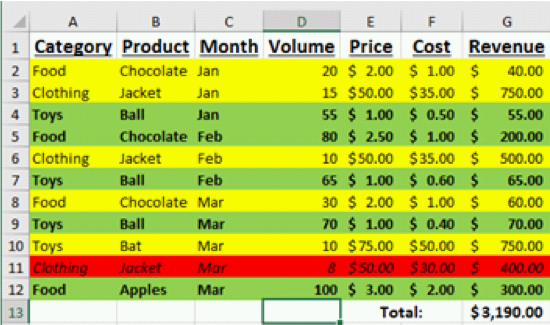
\includegraphics[width=0.45\textwidth]{excel1}  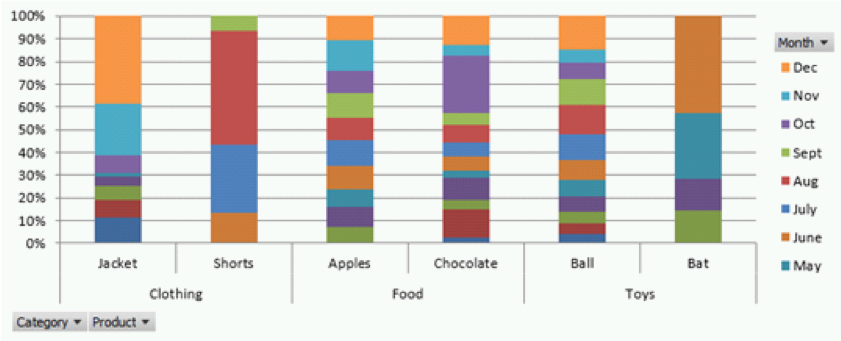
\includegraphics[width=0.45\textwidth]{excel2}
 
  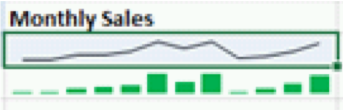
\includegraphics[width=0.3\textwidth]{excel3}
\caption{Examples of data visualizations using Excel}
\label{default}
\end{center}
\end{figure}

\end{frame}



\begin{frame}\ft{Data Visualization in Python}
Using Python a variety of charting libraries are available including {\tt matplotlib} and {\tt ggplot}.
\begin{figure}[htbp]
\begin{center}
 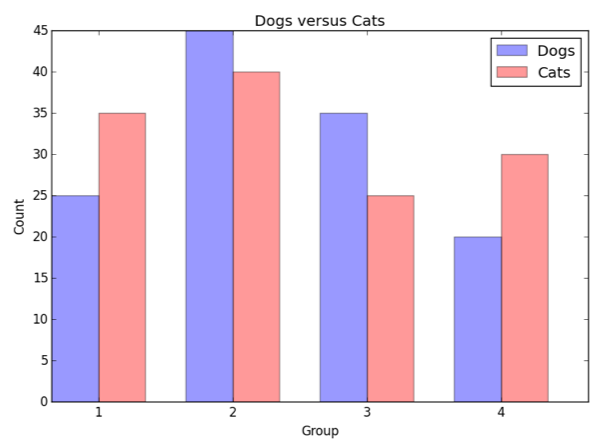
\includegraphics[width=0.45\textwidth]{python1}  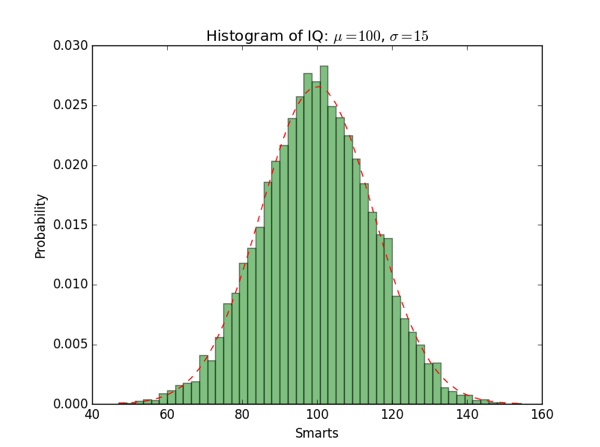
\includegraphics[width=0.45\textwidth]{python2}
\caption{Examples of data visualizations using Python}
\label{default}
\end{center}
\end{figure}

\end{frame}

\begin{frame}\ft{Data Visualization in R - Qualitative Data}
Using in R we can create visualization for qualitative data in form of bar charts, frequency tables, pie charts,
\begin{figure}[htbp]
\begin{center}
 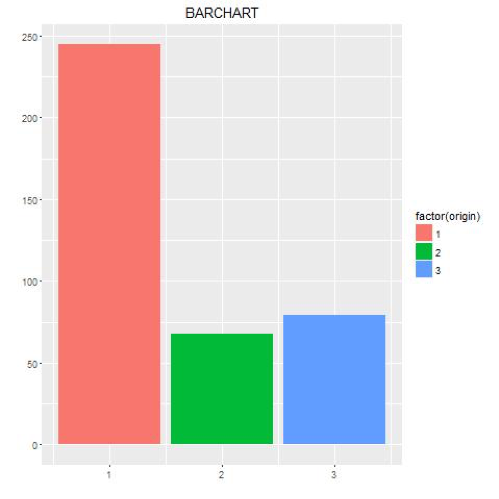
\includegraphics[width=0.4\textwidth]{r1}  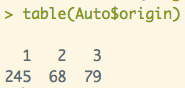
\includegraphics[width=0.2\textwidth]{r2}
 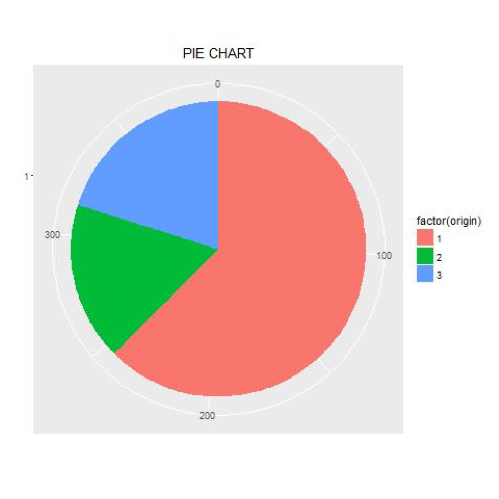
\includegraphics[width=0.4\textwidth]{r3}
\caption{Examples of qualitative data visualizations using {\tt ggplot} in {\tt R}}
\label{default}
\end{center}
\end{figure}

\end{frame}


\begin{frame}\ft{Data Visualization in R - Quantitative Data}
Using in R we saw examples of how we could represent quantitative data, eg. histograms, boxplots%, ECDF
\begin{figure}[htbp]
\begin{center}
 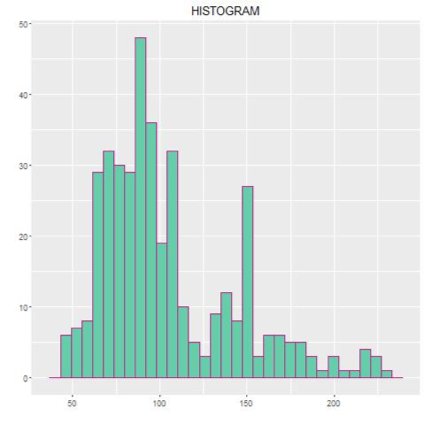
\includegraphics[width=0.4\textwidth]{r4}  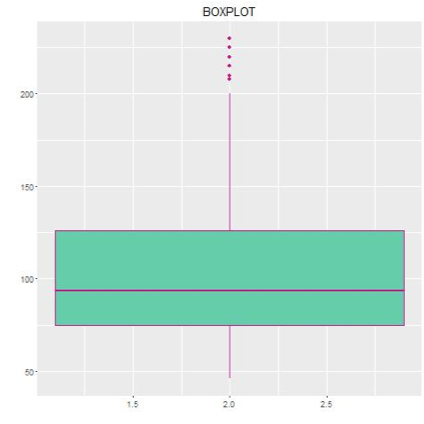
\includegraphics[width=0.4\textwidth]{r5}
% 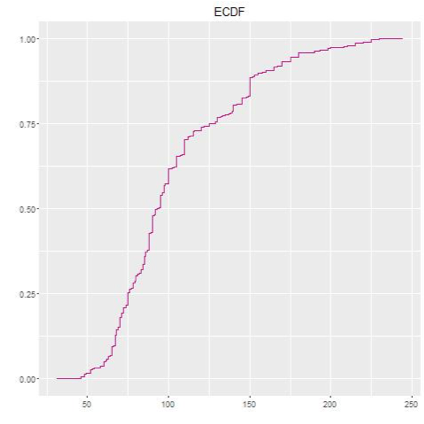
\includegraphics[width=0.4\textwidth]{r6}
\caption{Examples of quantitative data visualizations using R}
\label{default}
\end{center}
\end{figure}
\end{frame}

\begin{frame}{}
\begin{itemize}
\item The last two slides demonstrate how the importance of the \textit{type} of data being inputted into our graphics.
\vfill
\item Namely the collection of graphs we could create with qualitative data is different from the collection of graphs we could make with quantitative data.
\vfill
\item \emph{Tableau} is a \alert{\underline{very}} powerful tool for data visualization, that will do a lot of the heavy lifting  and allow us to gain deeper insights into our data. \vfill
\item Tableau will help us guide us along the way by segregating qualitative from quantitative fields and provide suggestions on useful types of graphics depending on the inputted fields.
\vfill 
\end{itemize}
\end{frame}


%\begin{frame}\ft{Data Visualization in GIS}
%Using GIS, we can visualize data in maps of coordinates with overlays (markers, points, lines, regions)
%\begin{figure}[htbp]
%\begin{center}
% 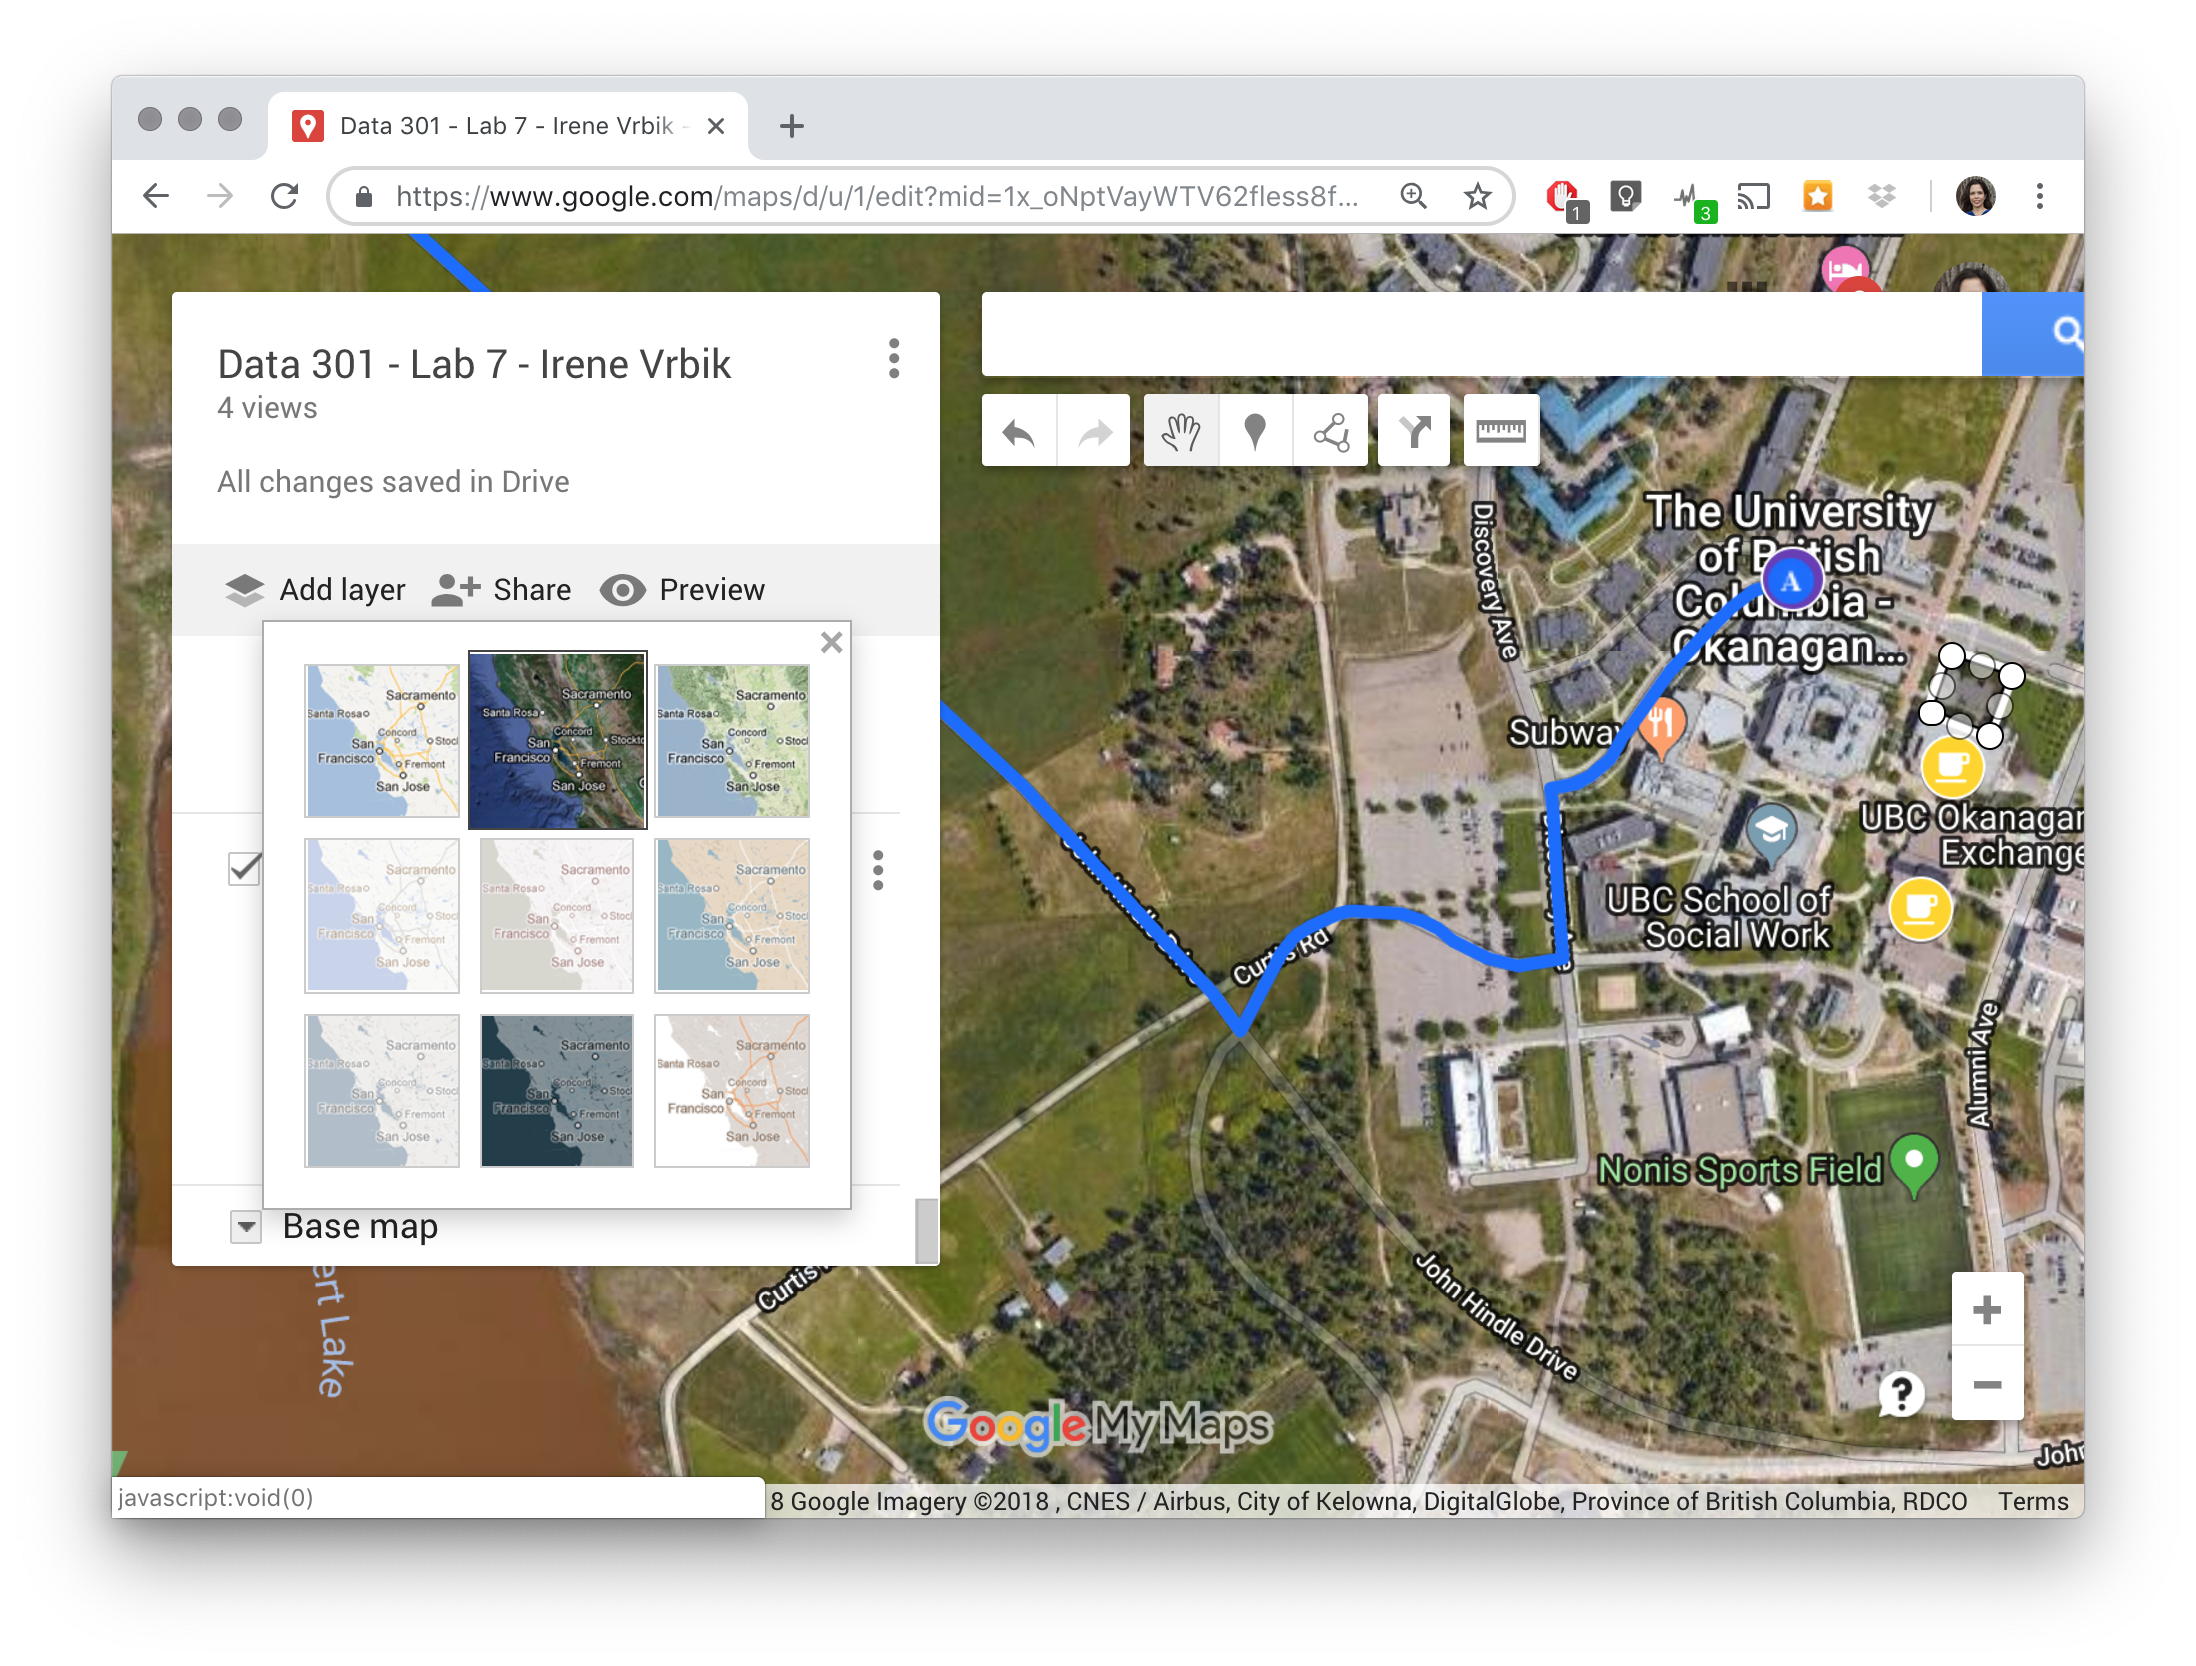
\includegraphics[height=0.5\textheight]{satelite}  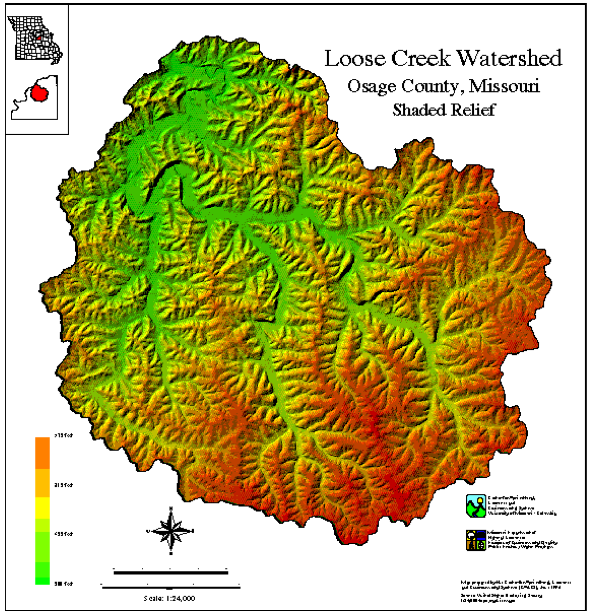
\includegraphics[height=0.45\textheight]{GIS2}
%\caption{Examples of visualizations using GIS}
%\label{default}
%\end{center}
%\end{figure}
%
%\end{frame}


%%https://tdwi.org/articles/2016/05/17/understand-knowns-and-unknowns-in-data.aspx
%
%\begin{frame}\ft{Types of Data}
%%Effective data preparation depends on recognizing how to handle what we know and what we don't know about a set of data. 
%Data can be considered of three types:\vfill
%\begin{description}
%\item[Known data] monitoring and regular reporting data for visibility
%\item[Data You Know You Need] for understanding outliers or trends in the known data and deciding on how to act on them
%\item[Data You Need but Do Not Know It] information that you would have not thought about but knowing it would be very valuable (data to discover!)
%\end{description}
%Visual analytics helps with all three types of data, but especially the last two to understand trends and discover important information.\vfill
%
%
%\end{frame}
%
%
%
%\frame{
%\ft{Types of Data}
%For example, if we think about this from a regression or classification standpoint we might have some explanatory variables (attributes) and response variable (instances) which may or may not be known.  \vfill
%How we approach these problems will depend on the data,\dots
%\begin{center}
%\begin{tabular}{|r|r|c|c|}
%\hline
%\multicolumn{2}{|c|}{}& \multicolumn{2}{c|}{Instances}\\
%\cline{3-4}
%\multicolumn{2}{|c|}{}&\textbf{Known}  & \textbf{Unknown}\\
%\hline
%\multirow{5}{*}{Attributes} 
%	&\multirow{2}{*}{\textbf{Known}} & {Known-known} & {Known-Unknown} \\
%	&& (discriminant analysis)& (clustering)\\
%	\cline{2-4}
%	&\multirow{3}{*}{\textbf{Unknown}} & \textcolor{gray}{Unknown-known} & {Unknown-unknown}\\
%	&&(data collection)& (variable selection)\\
%		&&& /clustering)\\
%\hline
%\end{tabular}
%\end{center}
%
%}

%\begin{frame}\ft{Introduction to Tableau}
%\begin{itemize}
%\end{itemize}
%
%\end{frame}


\begin{frame}\ft{Introduction to Tableau}
\begin{itemize}
\item \href{http://www.tableau.com/}{Tableau} was founded in 2003 as a spin-off from Stanford University by Chris Stolte, Christian Chabot and Pat Hanrahan.\vfill
%\begin{itemize}
%\item \href{https://www.tableau.com/about/press-releases/2018/tableau-reports-third-quarter-2018-financial-results}{2018} revenue was over \$650 million with over 3000 employees\vfill
%\end{itemize}

\item The goal of Tableau is "to help people see and understand their data." - Christian Chabot, Tableau CEO\vfill
\begin{itemize}
\item \alert{General goal}: make less unknown and more known.\vfill
\item Graphical representation of data can allow us to see patterns that we may not necessarily see by examining the raw data.\vfill
\end{itemize}


\item Tableau has desktop and server (enterprise) products as well as Tableau Public allowing sharing of data sets.
\vfill
\end{itemize}
\end{frame}



\begin{frame}\ft{Getting Started}
\begin{itemize}
\item We will be using the desktop version of \href{https://www.tableau.com/academic/students}{Tableau}
\vfill
\item Visit \href{https://www.tableau.com/academic/students}{this} site to obtain a license or to view examples of its use.
\vfill
\item We will be working with the Superstore data sets (Global Superstore Returns 2016.csv and Global Superstore Orders 2016.xlsx).\vfill
\item The quickest way to download this data is to click the ``Getting Started" video located on Tableau \hyperlink{homepage}{home page} or \href{https://www.tableau.com/learn/tutorials/on-demand/getting-started?product=all&version=tableau\_desktop\_2019\_1\&topic=getting\_started}{here} (you will need to register and sign in before you can see the videos).
\vfill
%\item In today's demo, you will see how quickly and easy it can be to make both {statitic}  and \textit{interactive} graphics in Tableau. \vfill 
\end{itemize}
\end{frame}



\begin{frame}
\ft{Tableau Home page}\label{homepage}
\begin{center}
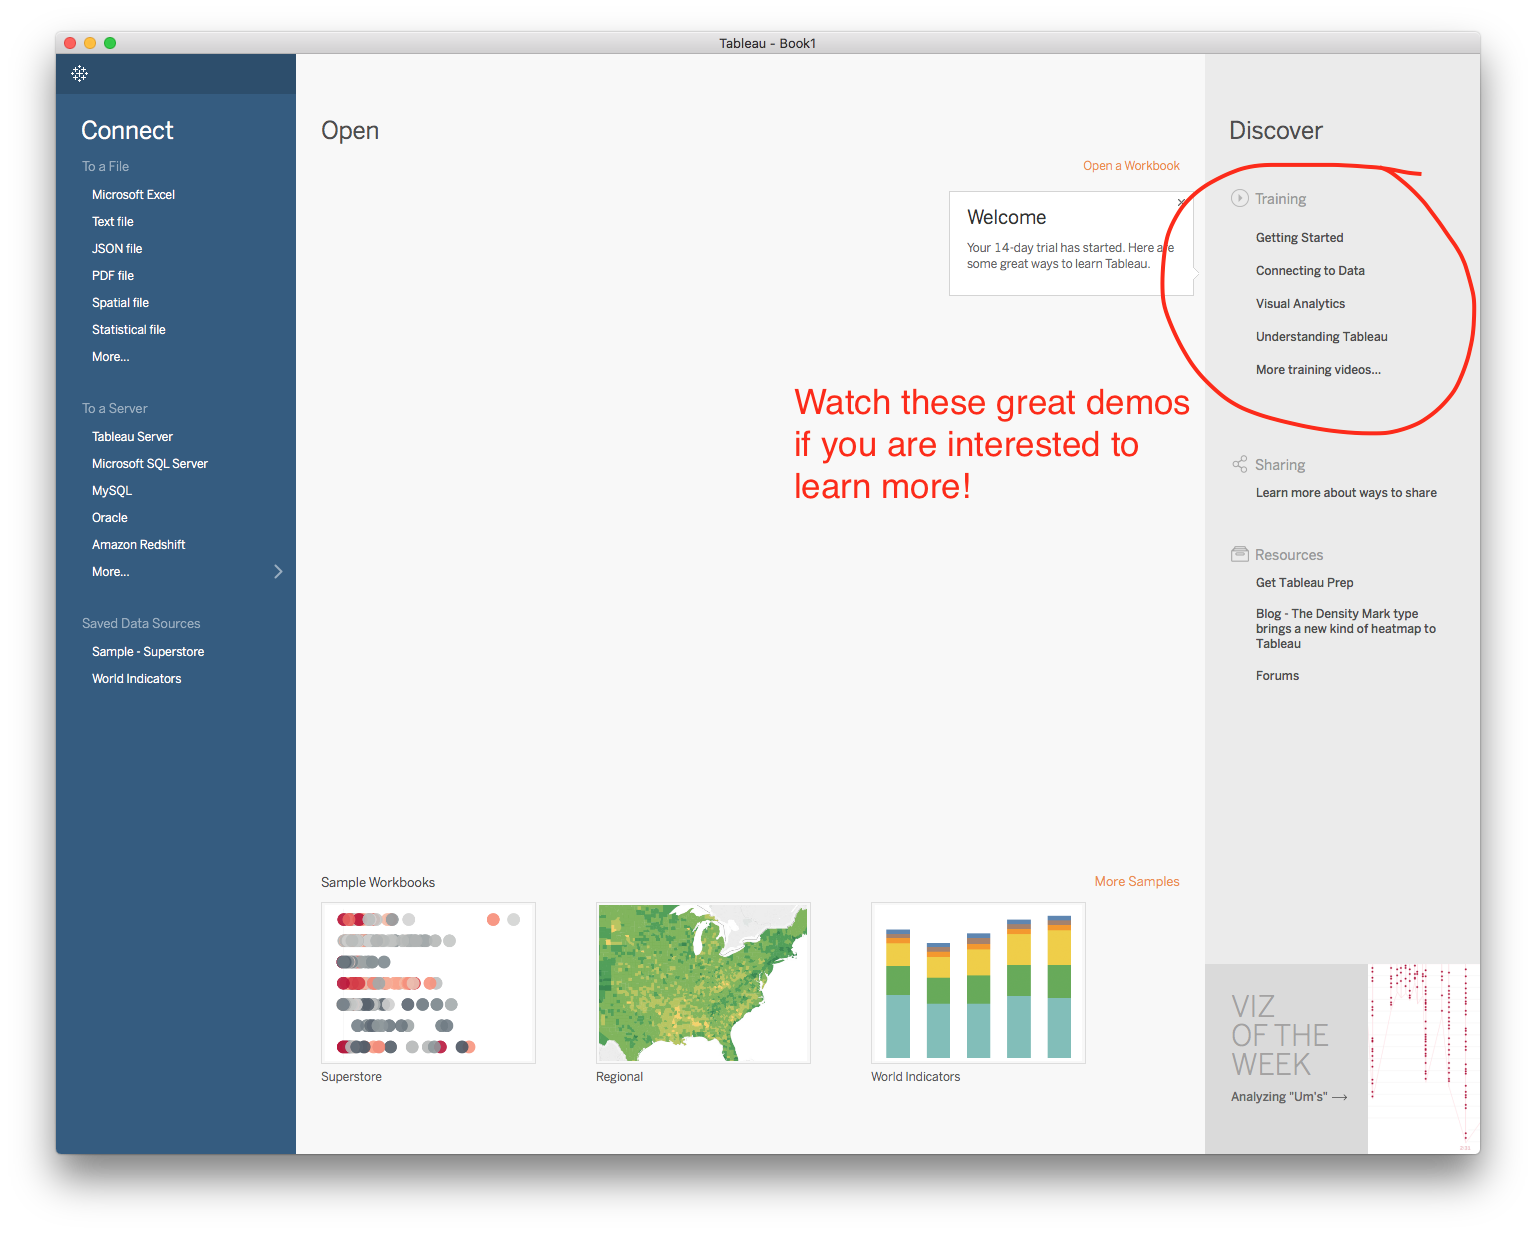
\includegraphics[width=0.9\textwidth]{img/home.png}
\end{center}
\end{frame}


%\begin{frame}\ft{Introduction to Tableau}
%\begin{itemize}
%\item 
%\end{itemize}
%\end{frame}

\begin{frame}\ft{Home Page Tableau}
\begin{itemize}
\item On the right hand panel of the Home page, you will notice a series of instructional videos.\vfill
\item These are a great resource to learn more about the features available in Tableau.\vfill
\item See the training videos which use the Superstore data sets
\begin{itemize}
\item Global Superstore Orders 2016.xlsx
\item Global Superstore Returns 2016.csv
\end{itemize}
See finished workbook: getting\_started\_finished.twbx file\vfill
%\item These are accompanied by downloadable data on which to practice these techniques.\vfill
\item  On the left hand panel, you will notice that there are several ways that we can connect with data:
\begin{itemize}
\item stored locally on our computer (eg. excel files, .csv)
\item on a server (eg. MySQL)
\end{itemize}
\end{itemize}
\end{frame}




% https://www.superdatascience.com/blogs/why-learn-tableau
\begin{frame}\ft{Home Page Tableau}
\begin{itemize}
\item This requires that you have a license or trial key. \vfill
\item Students qualify for a free license through the Tableau for Students Program if currently enrolled at an accredited academic institution (undergraduate/post-graduate level).\vfill
\item The lab computers in SCI 234 should have Tableau installed (make sure you are using the latest version: Tableau 2019) \vfill
\item Sidenote: the Professional Version of Tableau is priced at \$1,999 + maintenance fee per license. 
\vfill
\item There is also a free version of their software called \href{https://public.tableau.com/en-us/s/}{Tableau Public.}

\end{itemize}
\end{frame}


%
%\begin{frame}
%\ft{Tableau Workspace}
%\begin{center}
%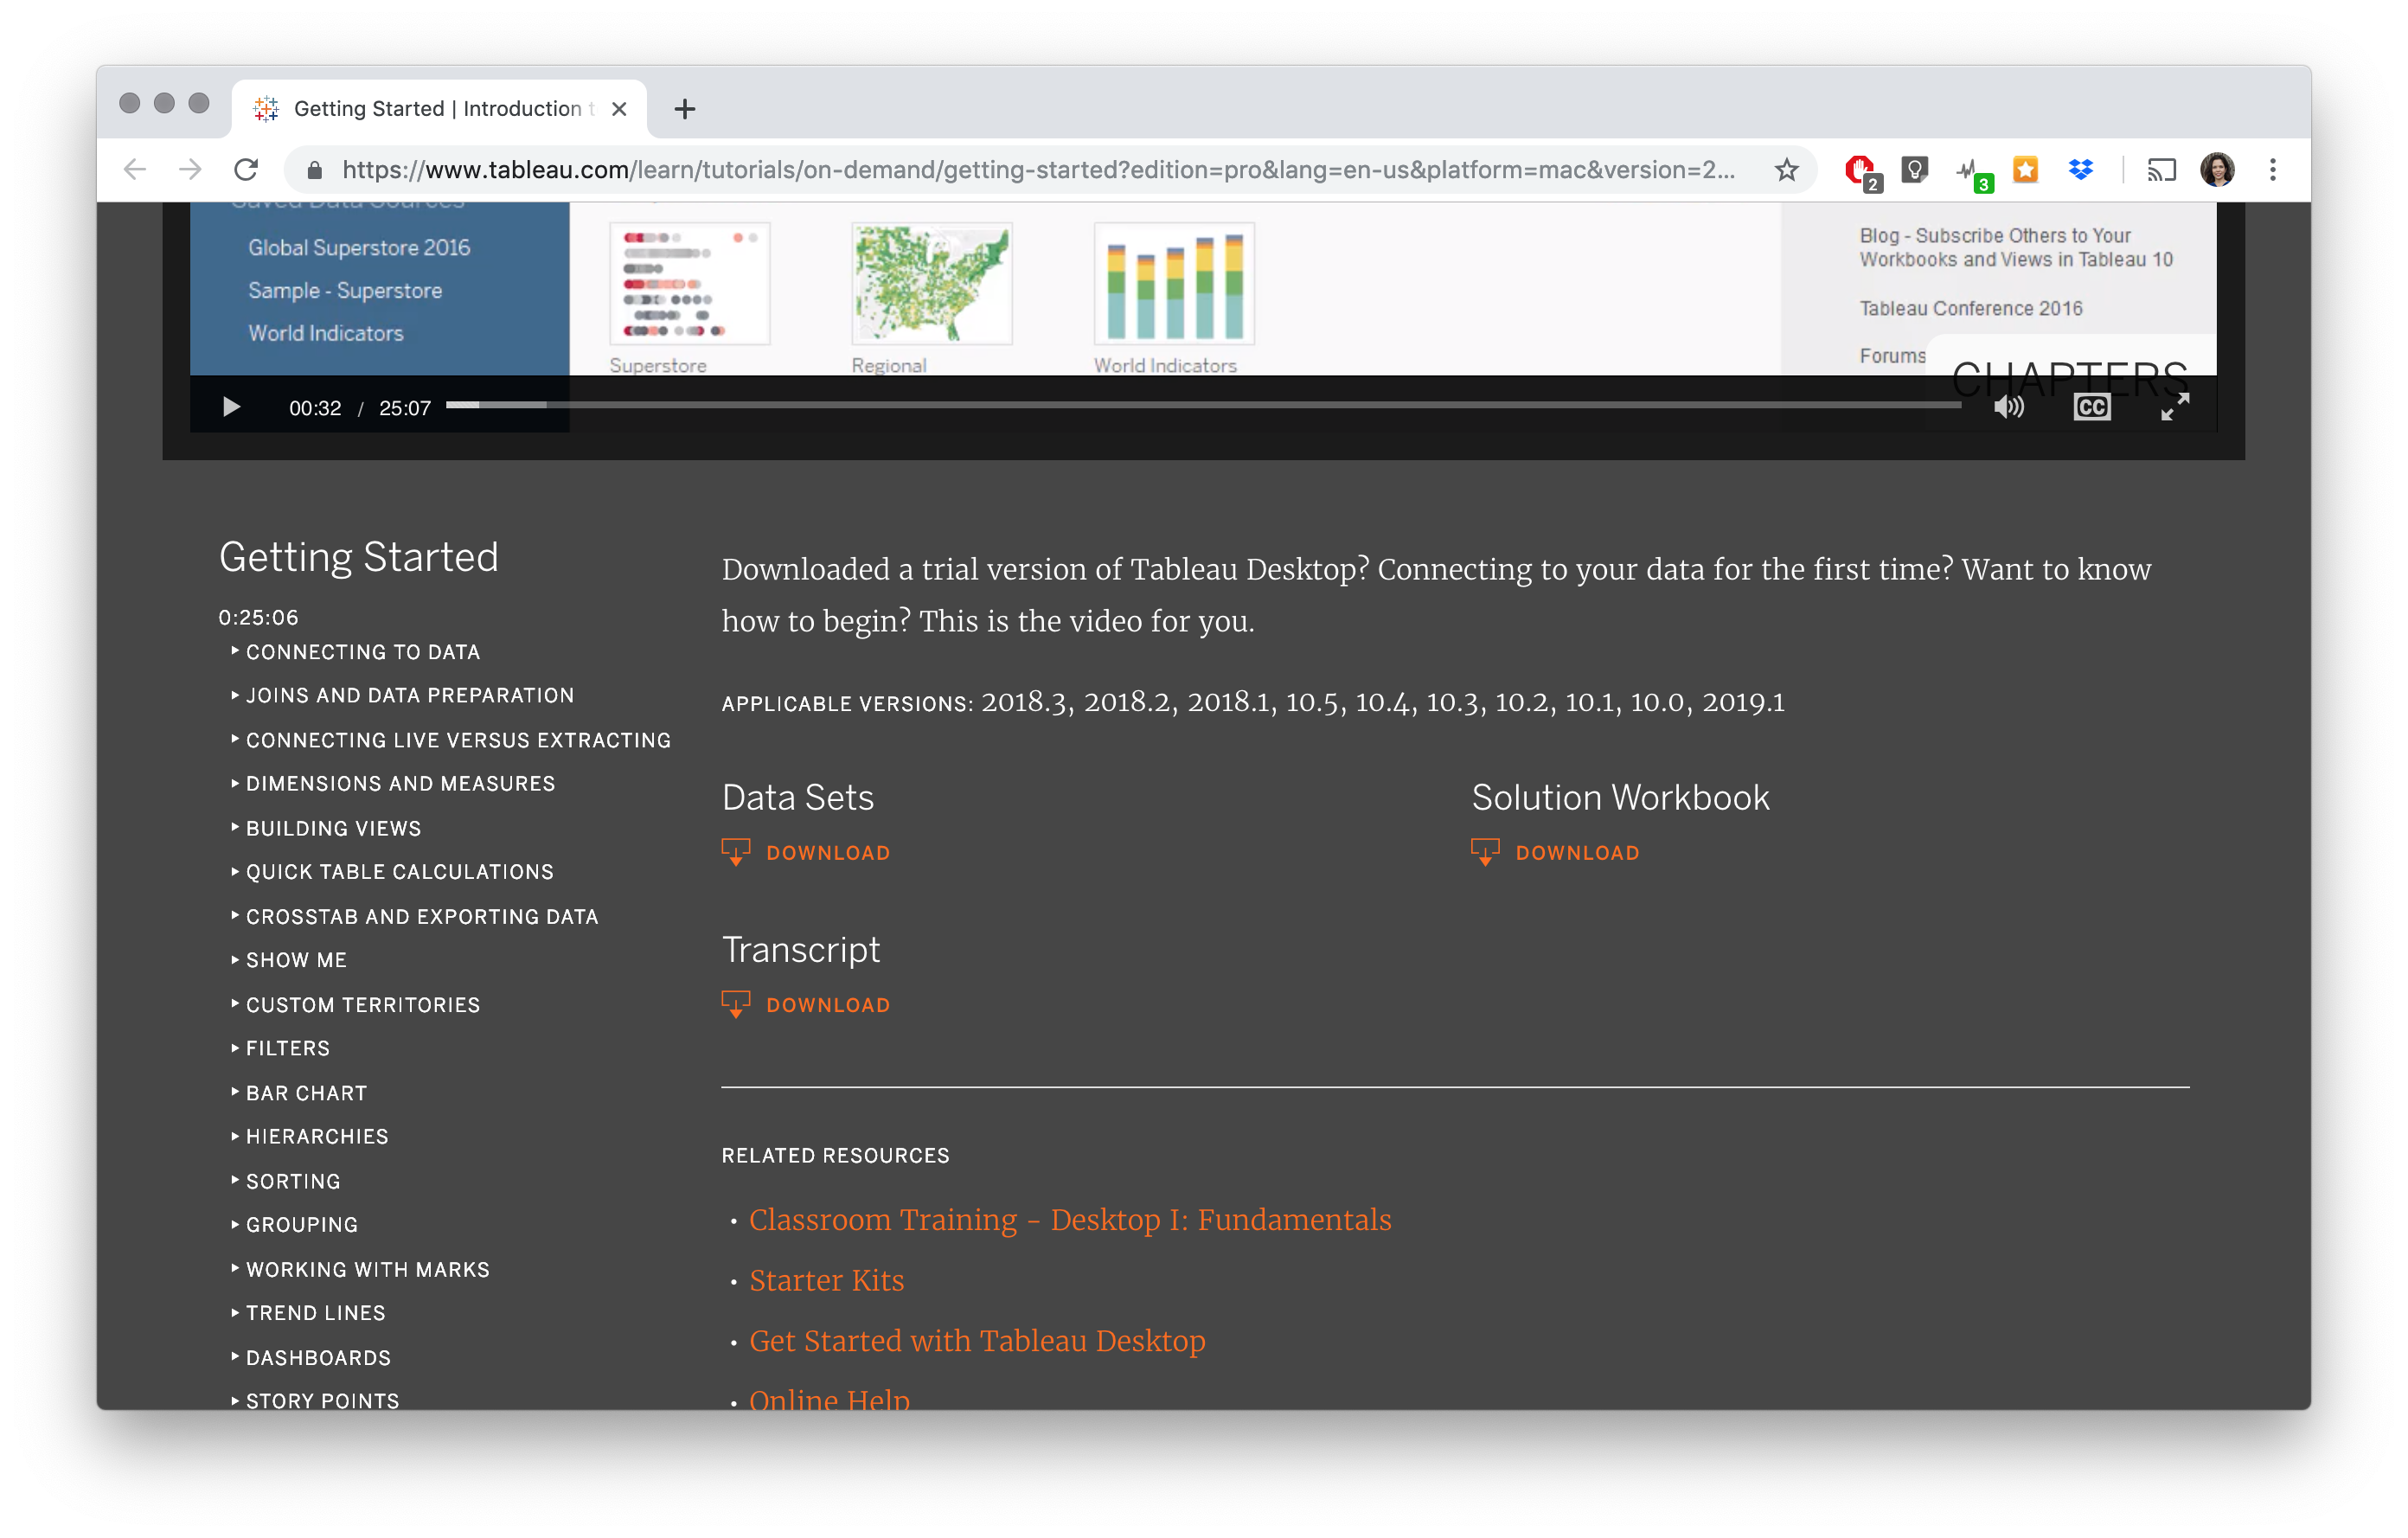
\includegraphics[width=0.9\textwidth]{img/gettingstarteddata}
%\end{center}
%\end{frame}


%\begin{frame}
%The excel file looks like this:
%\begin{center}
%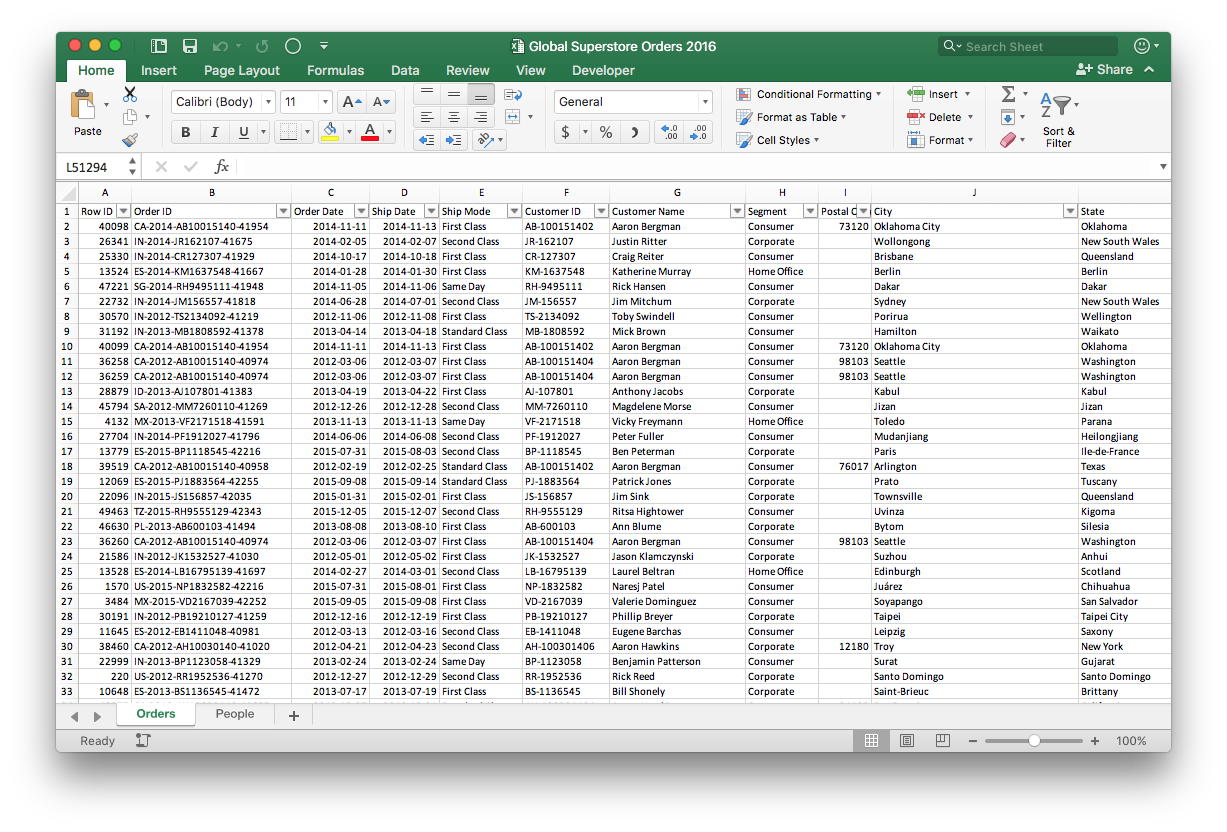
\includegraphics[width=0.9\textwidth]{img/superstroe}
%\end{center}
%\end{frame}
%
%\begin{frame}
%Notice it has two tabs:
%\begin{center}
%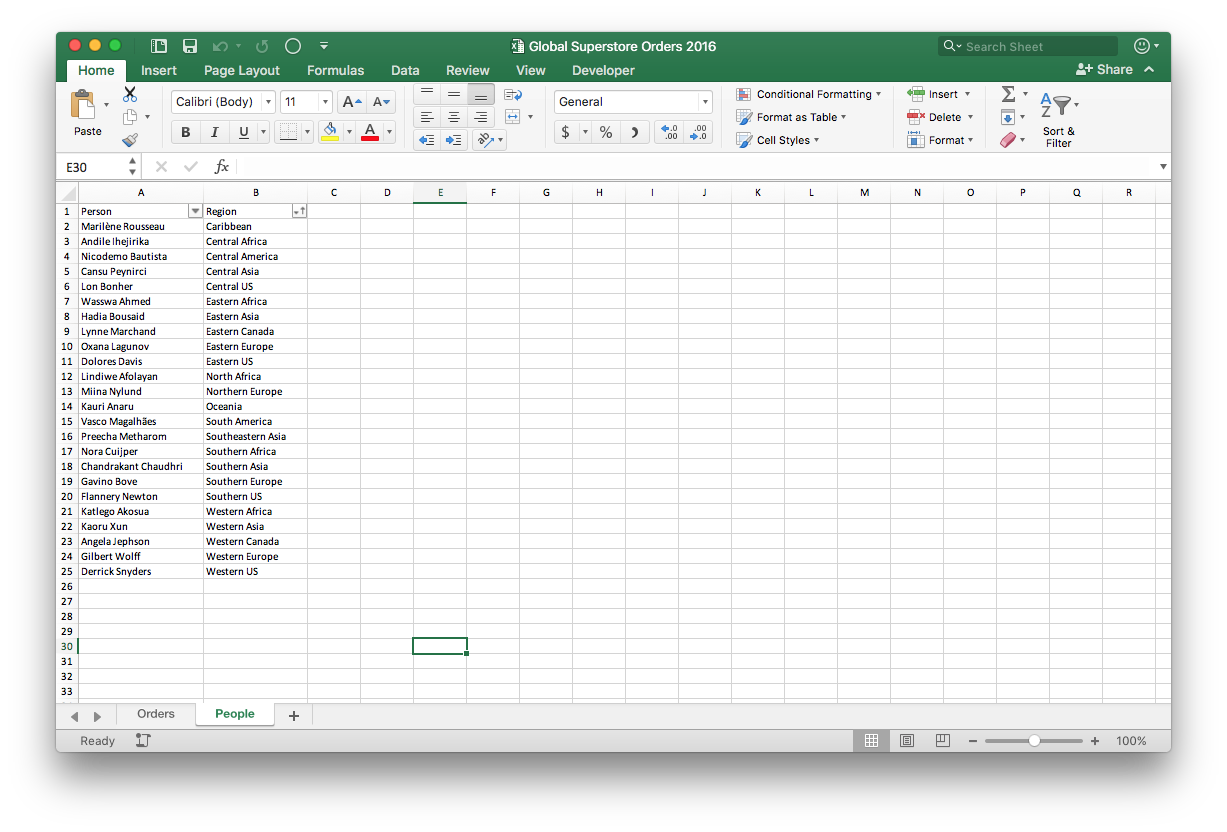
\includegraphics[width=0.9\textwidth]{img/people}
%\end{center}
%\end{frame}


\begin{frame}\ft{Superstore data}
\begin{itemize}
\item This excel file contains two tabs (ie two worksheets):
\begin{description}
\item[Orders]  which contains the products and transactions of customers.
\item[People] Customer information
\end{description}
\vfill

\item To begin, we read this file into Tableau by navigating to the Home Page > Connect (left panel) > To a file > Microsoft Excel.\vfill
\item This will open a data source page, from which we can drag and add different data sources.\vfill
\end{itemize}
\end{frame}

\begin{frame}
\ft{Tableau Workspace}
\begin{center}
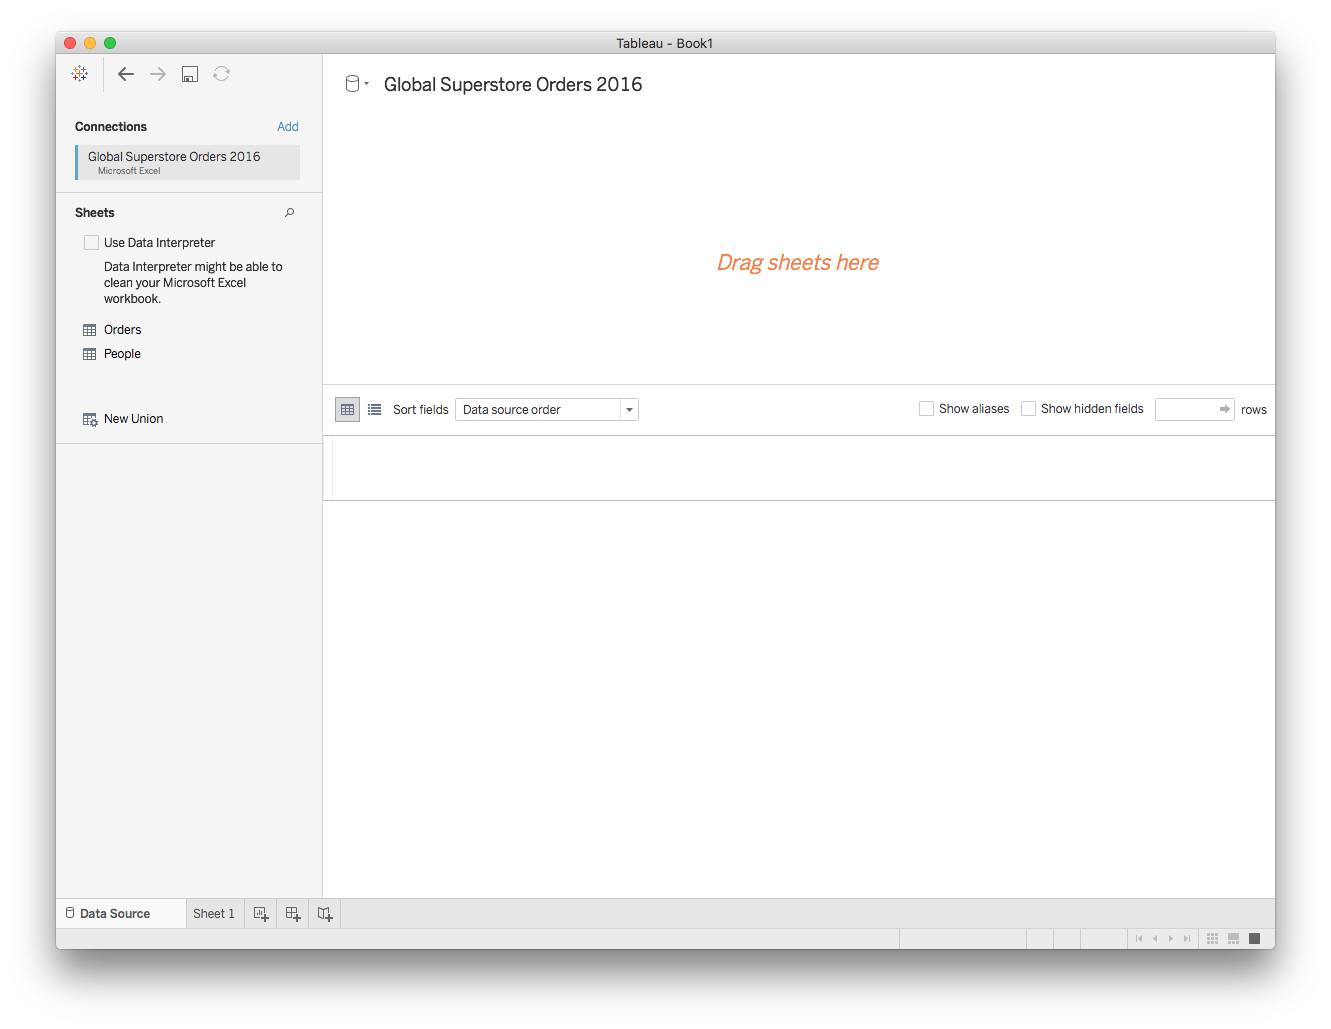
\includegraphics[width=0.9\textwidth]{img/datasource}
\end{center}
\end{frame}


\begin{frame}
\ft{Example Connecting to Excel}
\begin{center}
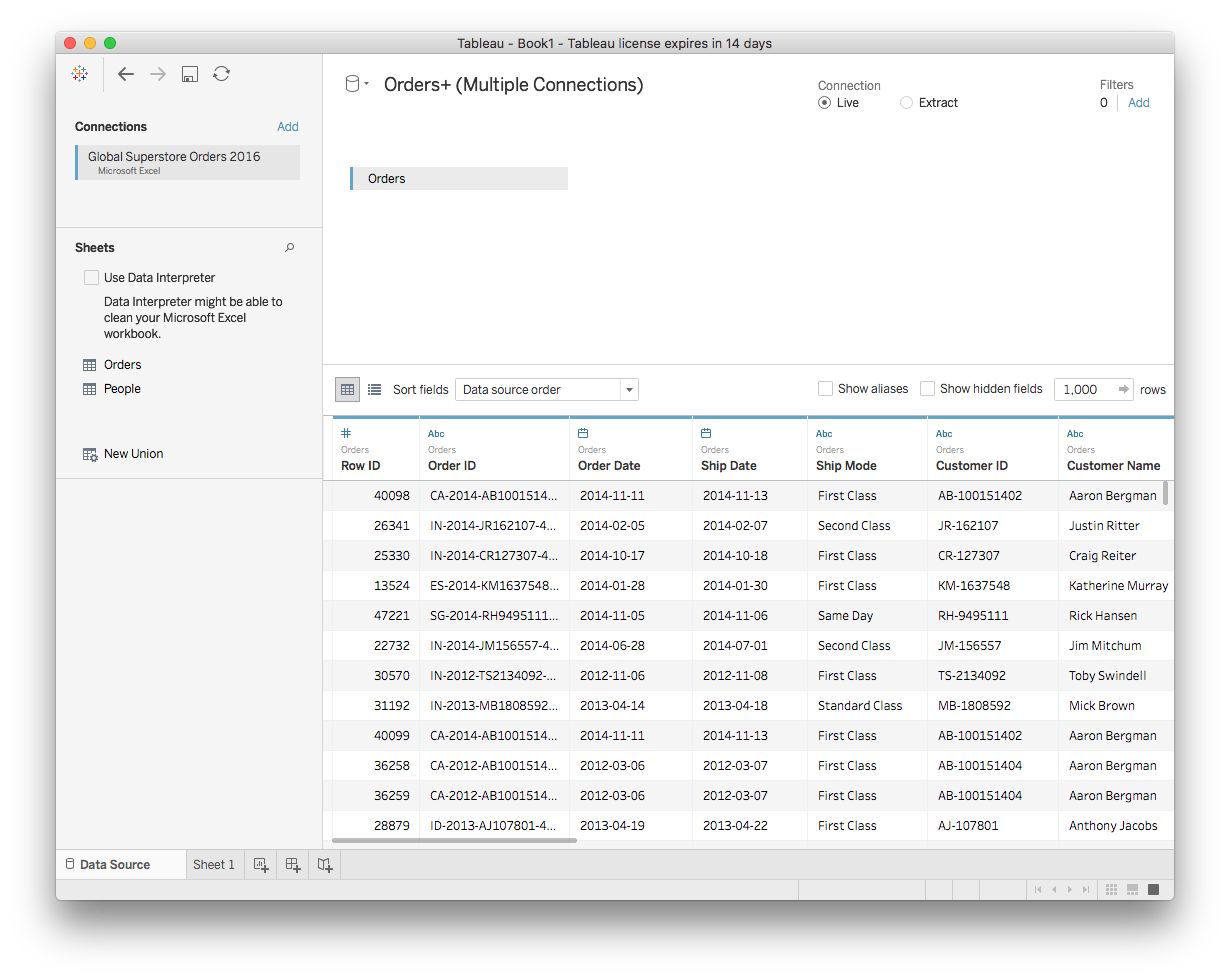
\includegraphics[width=.8\textwidth]{img/excel}
\end{center}
\end{frame}


\begin{frame}
\ft{Example Connecting to Excel}
\begin{itemize}

\item If we have {related} data in another data source, we can create an integrated data source by adding a connection, by clicking the ``Add" link in the top left corner.\vfill

\item For example, we can create a database-like JOIN with data from another source (eg. we can connect the Orders from Global Superstore Orders 2016.xlsx to the Returns from Global Superstore Returns 2016.csv)
\end{itemize}

\end{frame}






\begin{frame}
\ft{Tableau Workspace}
\begin{center}
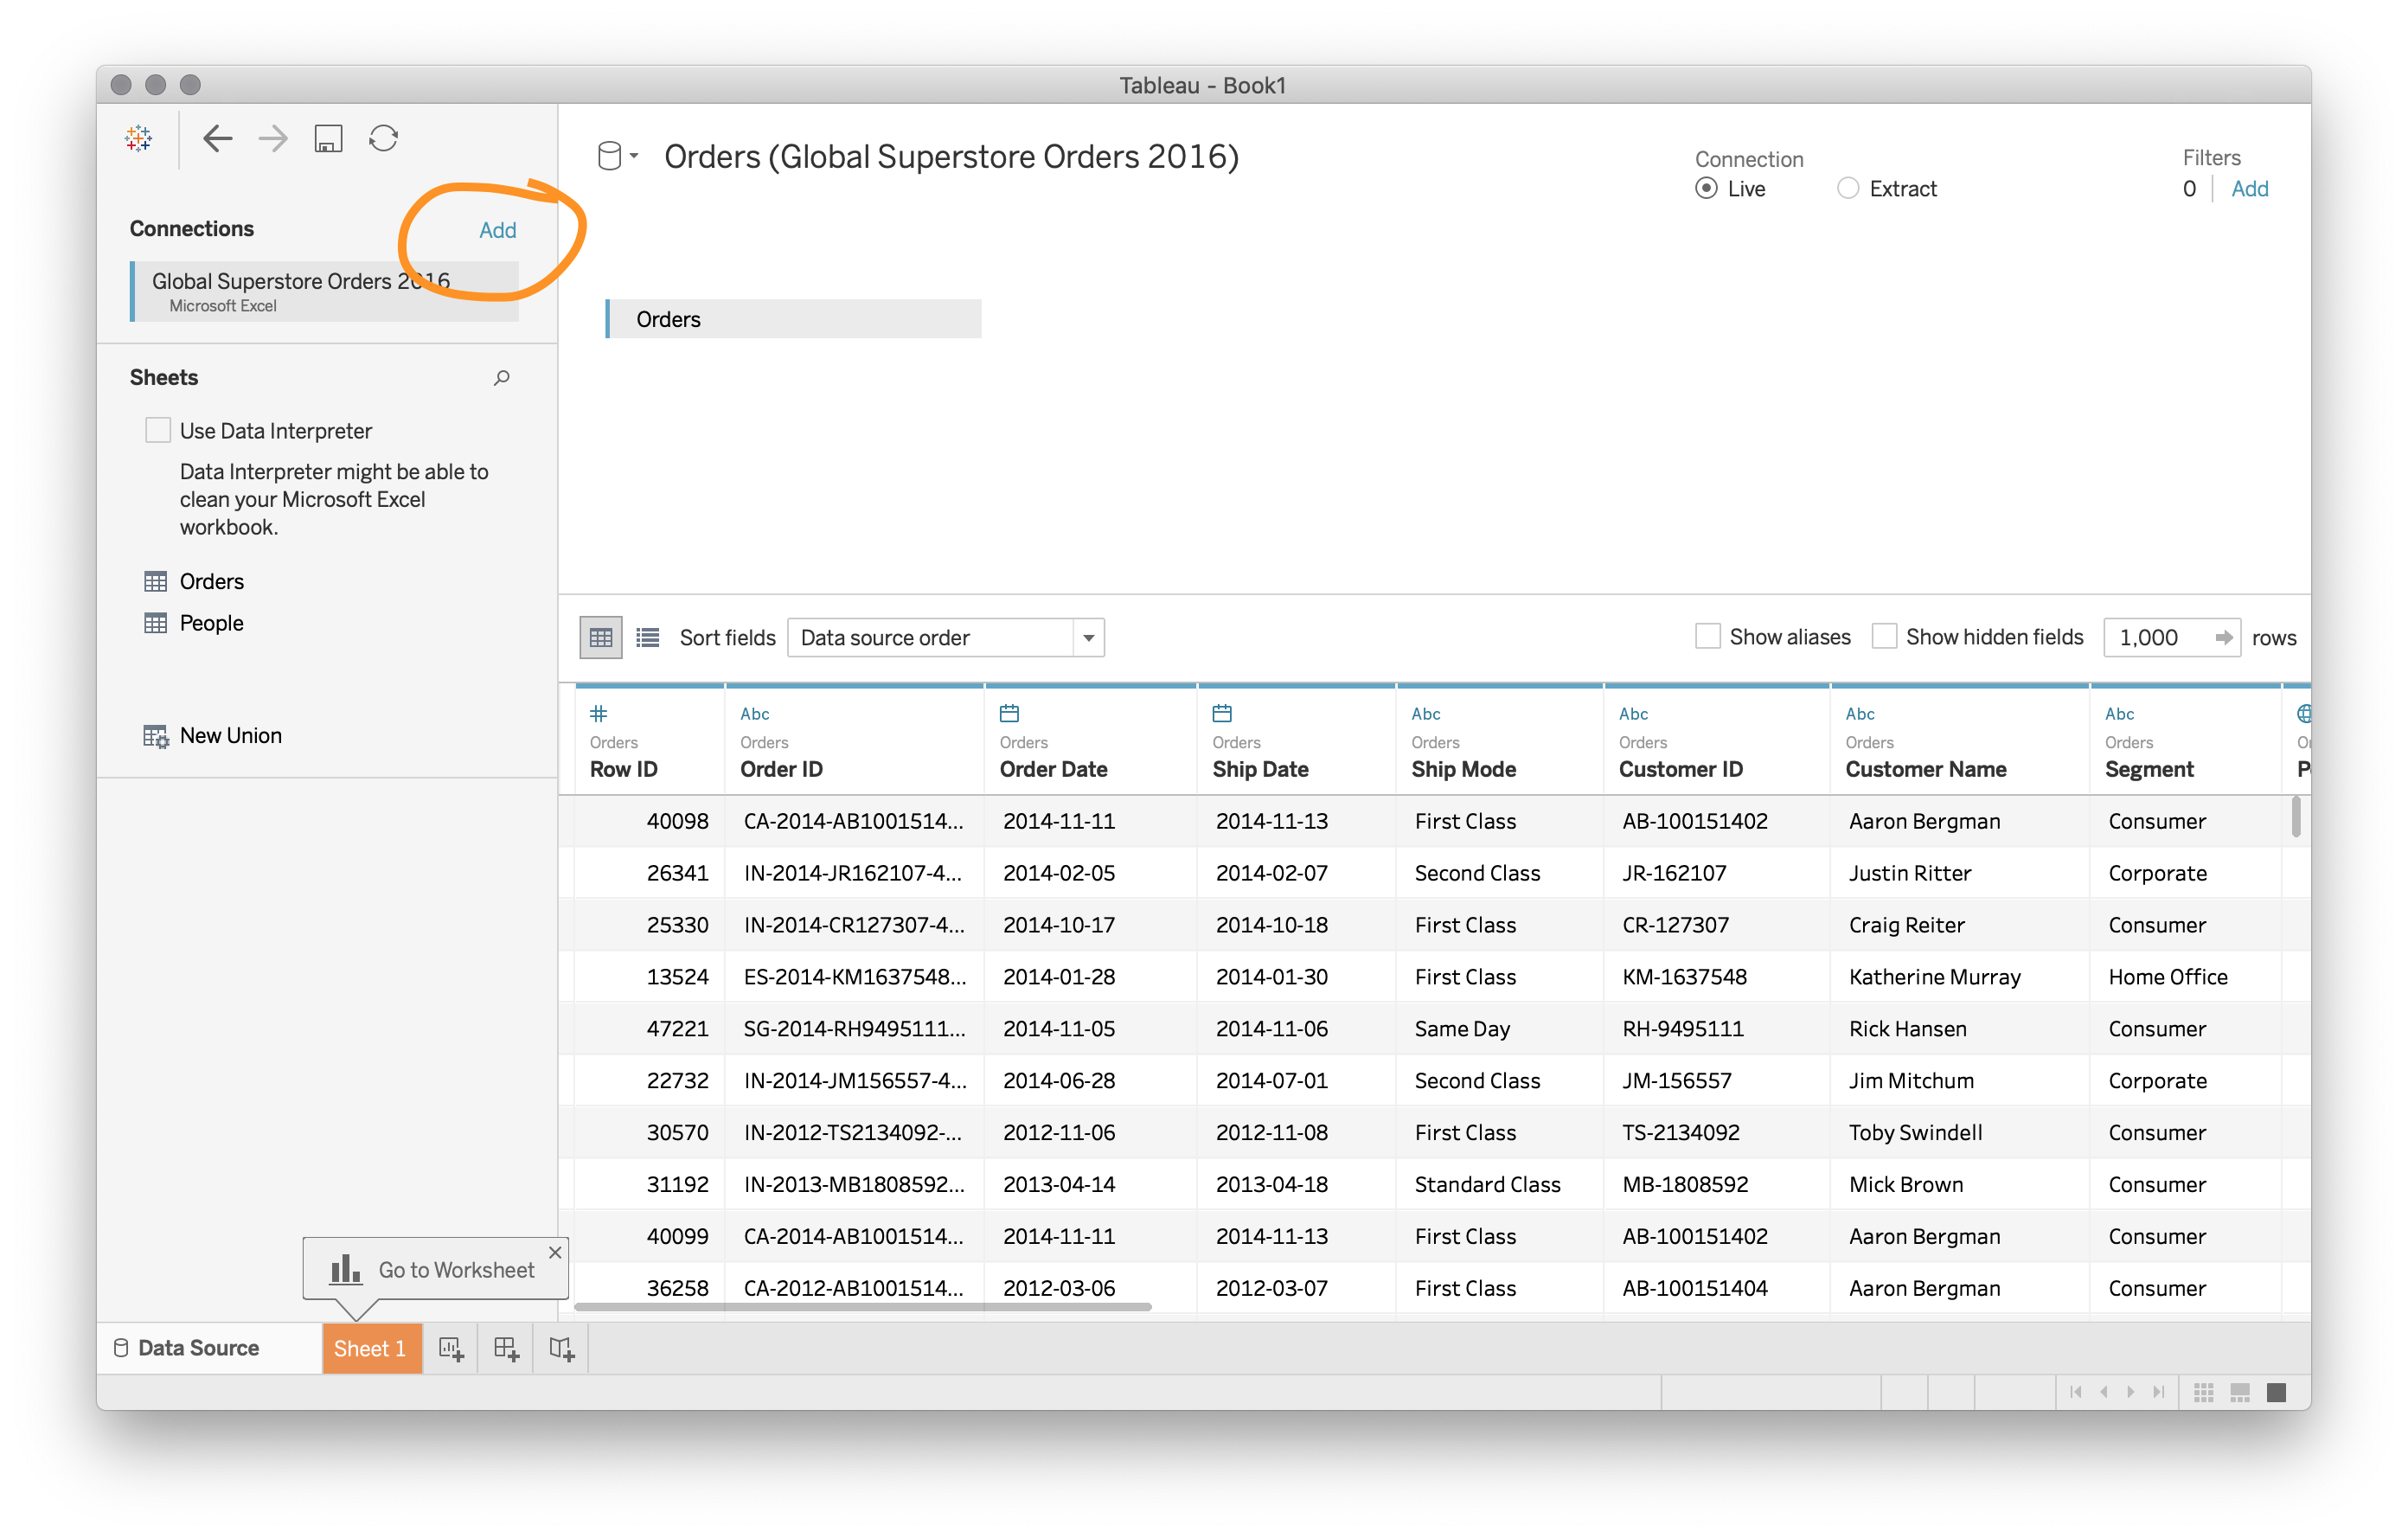
\includegraphics[width=0.9\textwidth]{img/add}
\end{center}
\end{frame}

\begin{frame}
\ft{Tableau Workspace}
Notice here that we have created a \alert{left join} (on {\tt Order ID}) which we can change by clicking on the Venn Diagram image.
\begin{center}
\includegraphics[width=0.9\textwidth]{img/leftjoin}
\end{center}
We can also change meta-data in the excel-like spreedsheet.
\end{frame}


\begin{frame}
Clicking on the `Sheet' tab (orange button in the lower left hand corner) will bring us to this workspace:
\ft{Tableau Workspace}
\begin{center}
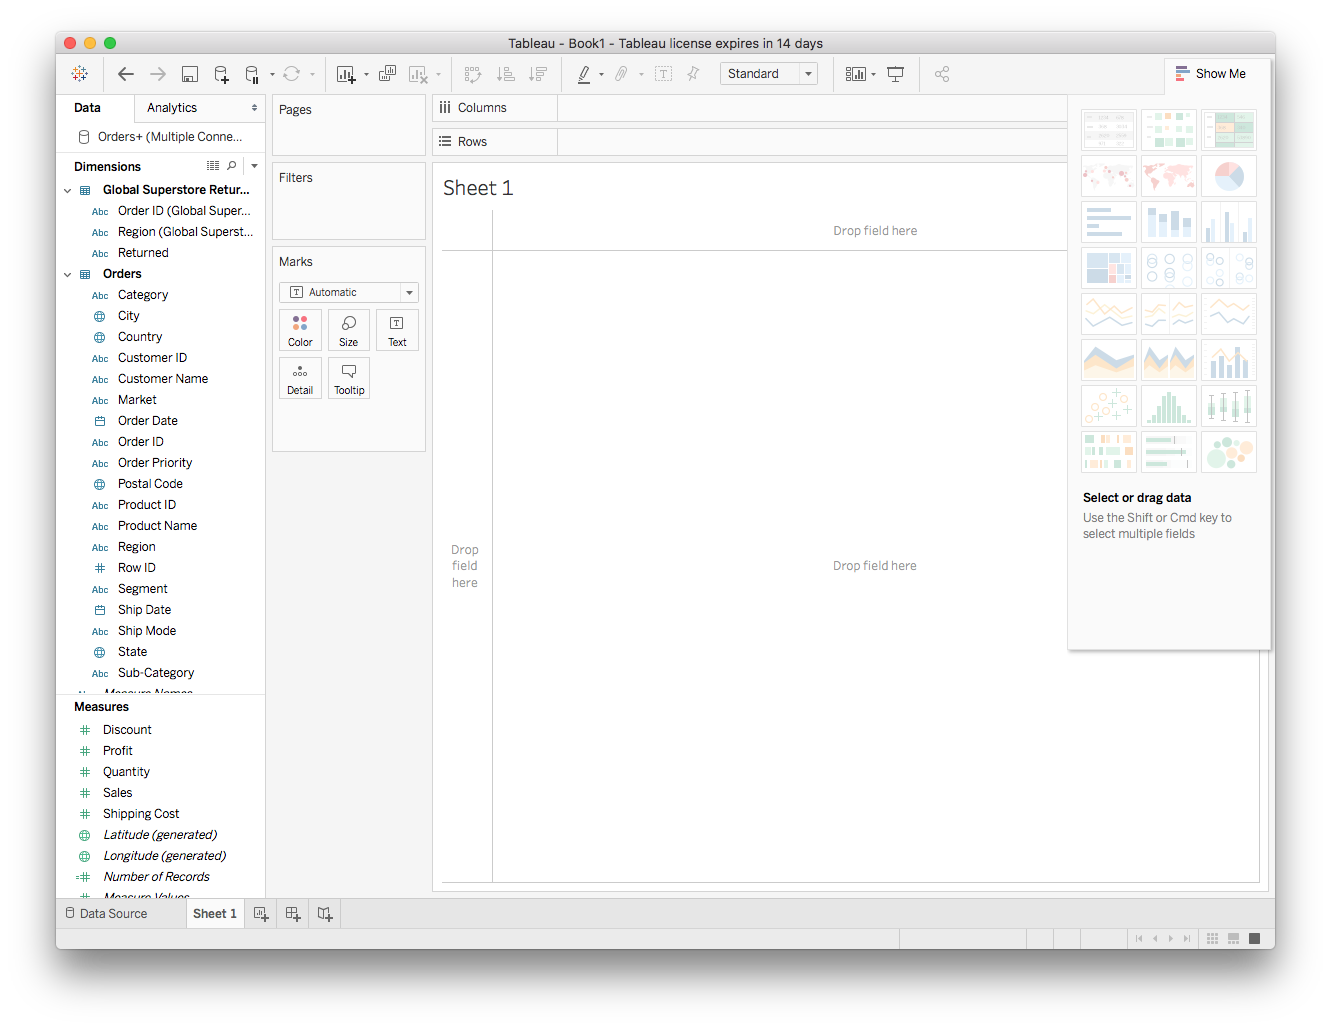
\includegraphics[width=0.9\textwidth]{img/workspace}
\end{center}
\end{frame}


\begin{frame}\ft{Tableau Features}
\begin{itemize}
\item Supported \href{https://onlinehelp.tableau.com/current/pro/desktop/en-us/datafields\_typesandroles\_datatypes.htm}{data types}: text 
\includegraphics[height=1em]{img/text}, dates 
\includegraphics[height=1em]{img/date}, numbers 
\includegraphics[height=1em]{img/number}, geographical coordinates 
\includegraphics[height=1em]{img/global} (latitude/longitude), Boolean 
\includegraphics[height=1em]{img/truefalse} \vfill

\item  There are a number of aggregation functions available in Tableau: sum, average, max, count, variance, etc.\vfill
\item There are many built-in functions for numeric and string manipulation.\vfill
\item Calculated fields can be created and are proceeded by an equal sign: 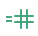
\includegraphics[height=1em]{img/calculated}\vfill
%% ^ dunno what that means
\item Visualizations are created by dragging these fields (or ``\textit{pills}") to desired \textit{shelves}, \dots 
\vfill
\end{itemize}
\end{frame}


\begin{frame}\ft{Tableau Terminology}
A \define{pill} is a field (i.e column in your data set) that can be placed in the visualization.  The are stored one of two \href{https://onlinehelp.tableau.com/current/pro/desktop/en-us/datafields\_typesandroles.htm}{field types}
\begin{columns}[T] % align columns
\begin{column}{.7\textwidth}
\begin{description}
\item [Dimension] or categorical/discrete information are colour-coded using \emph{blue} pills 
\item [Measures], that is, metrics containing our quantitative information are colour-coded using \emph{green} pills \vfill
\end{description}
\end{column}%
\hfill%
\begin{column}{.2\textwidth}
\vspace{1cm}
\hspace{-1cm}
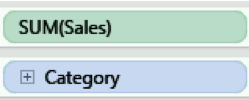
\includegraphics[width=1.3\textwidth]{img/pills.png}
\end{column}%
\end{columns}
\vspace{5mm}
Dimensions (eg. date, customer) are usually what is used for creating \textit{labels} while the Measures (eg price) are the metrics we want to analyze (this data is often continuous). 
\end{frame}

\begin{frame}\ft{Tableau Terminology}
A \define{shelf} is a location to put a pill.
\begin{itemize}
\item Column shelf, row shelf, filter shelf
\item Row and column shelves are similar to Pivot tables in Excel but with built-in visualization.\vfill
\end{itemize}
Dragging pills to different shelves will change the way our graphics appears.  To remove of undo a move, simple drag the pill off the shelf to delete, or press the undo button.  The Clear Sheet 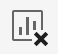
\includegraphics[height=1em]{img/clearsheet}~ button will erase the entire graphic 
\begin{center}
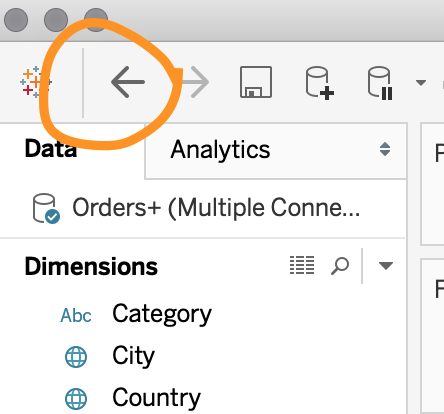
\includegraphics[width=.25\textwidth]{img/undo}
\end{center}
\end{frame}

\begin{frame}
\ft{Tableau Workspace Items}
\begin{center}
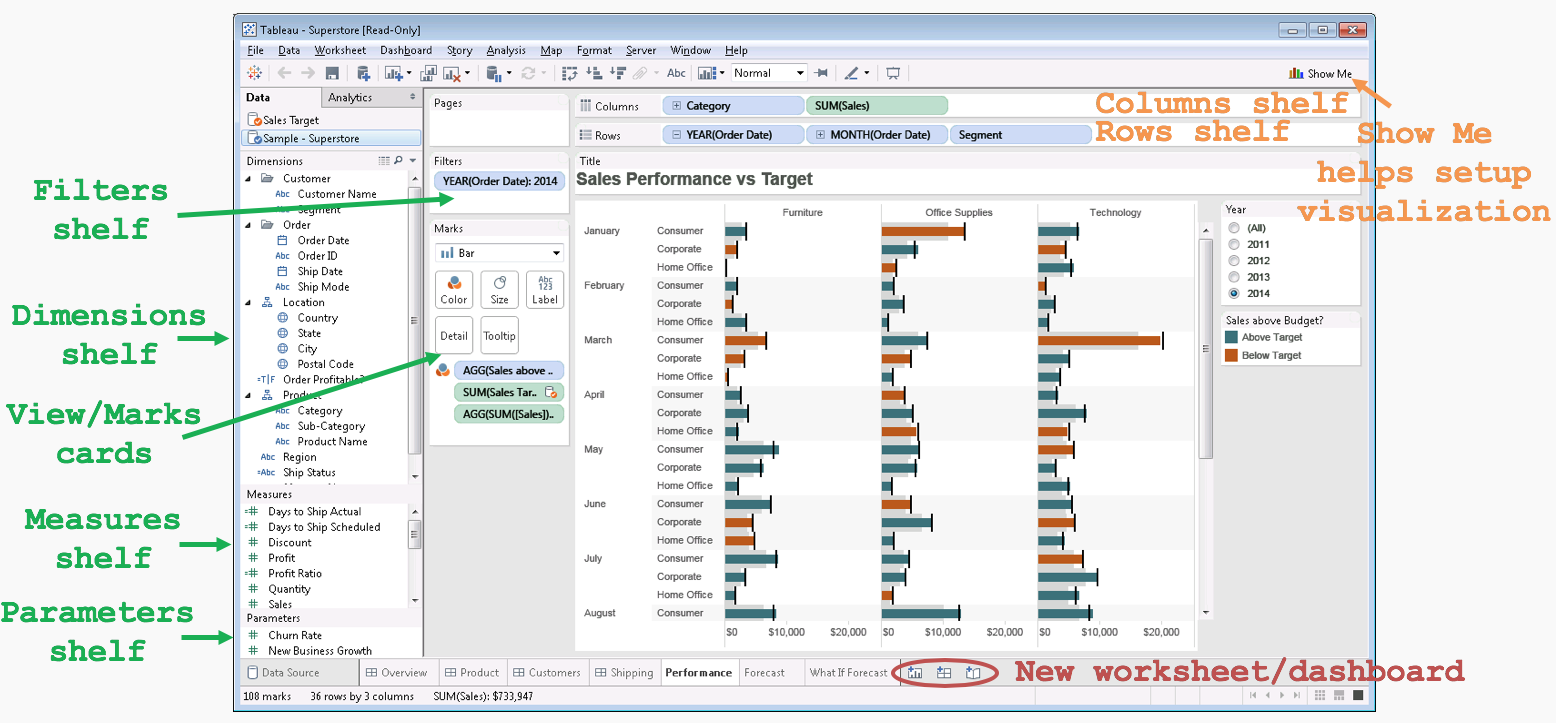
\includegraphics[width=1.05\textwidth]{img/workplaceitems}
\end{center}
\end{frame}



\begin{frame}\ft{View Cards}
View or shape cards allows control of colour, shape, and size. They also enable filtering, labeling, and ability to add details on demand.
\begin{description}
\item[Color] expresses discrete or continuous values
\item[Size] expresses discrete or continuous values
\item[Label] one or more fields can be expressed as label on marks
\item[Detail] disaggregates the marks plotted
\item[Tooltip] makes fields available to tooltips without disaggregating data (shows info when hovering)
\item [Shape]expresses discrete or continuous fields\vfill
\end{description}
Multiple fields can be placed on the colour, label, detail, and tooltip buttons.
\end{frame}



\begin{frame}
\begin{center}
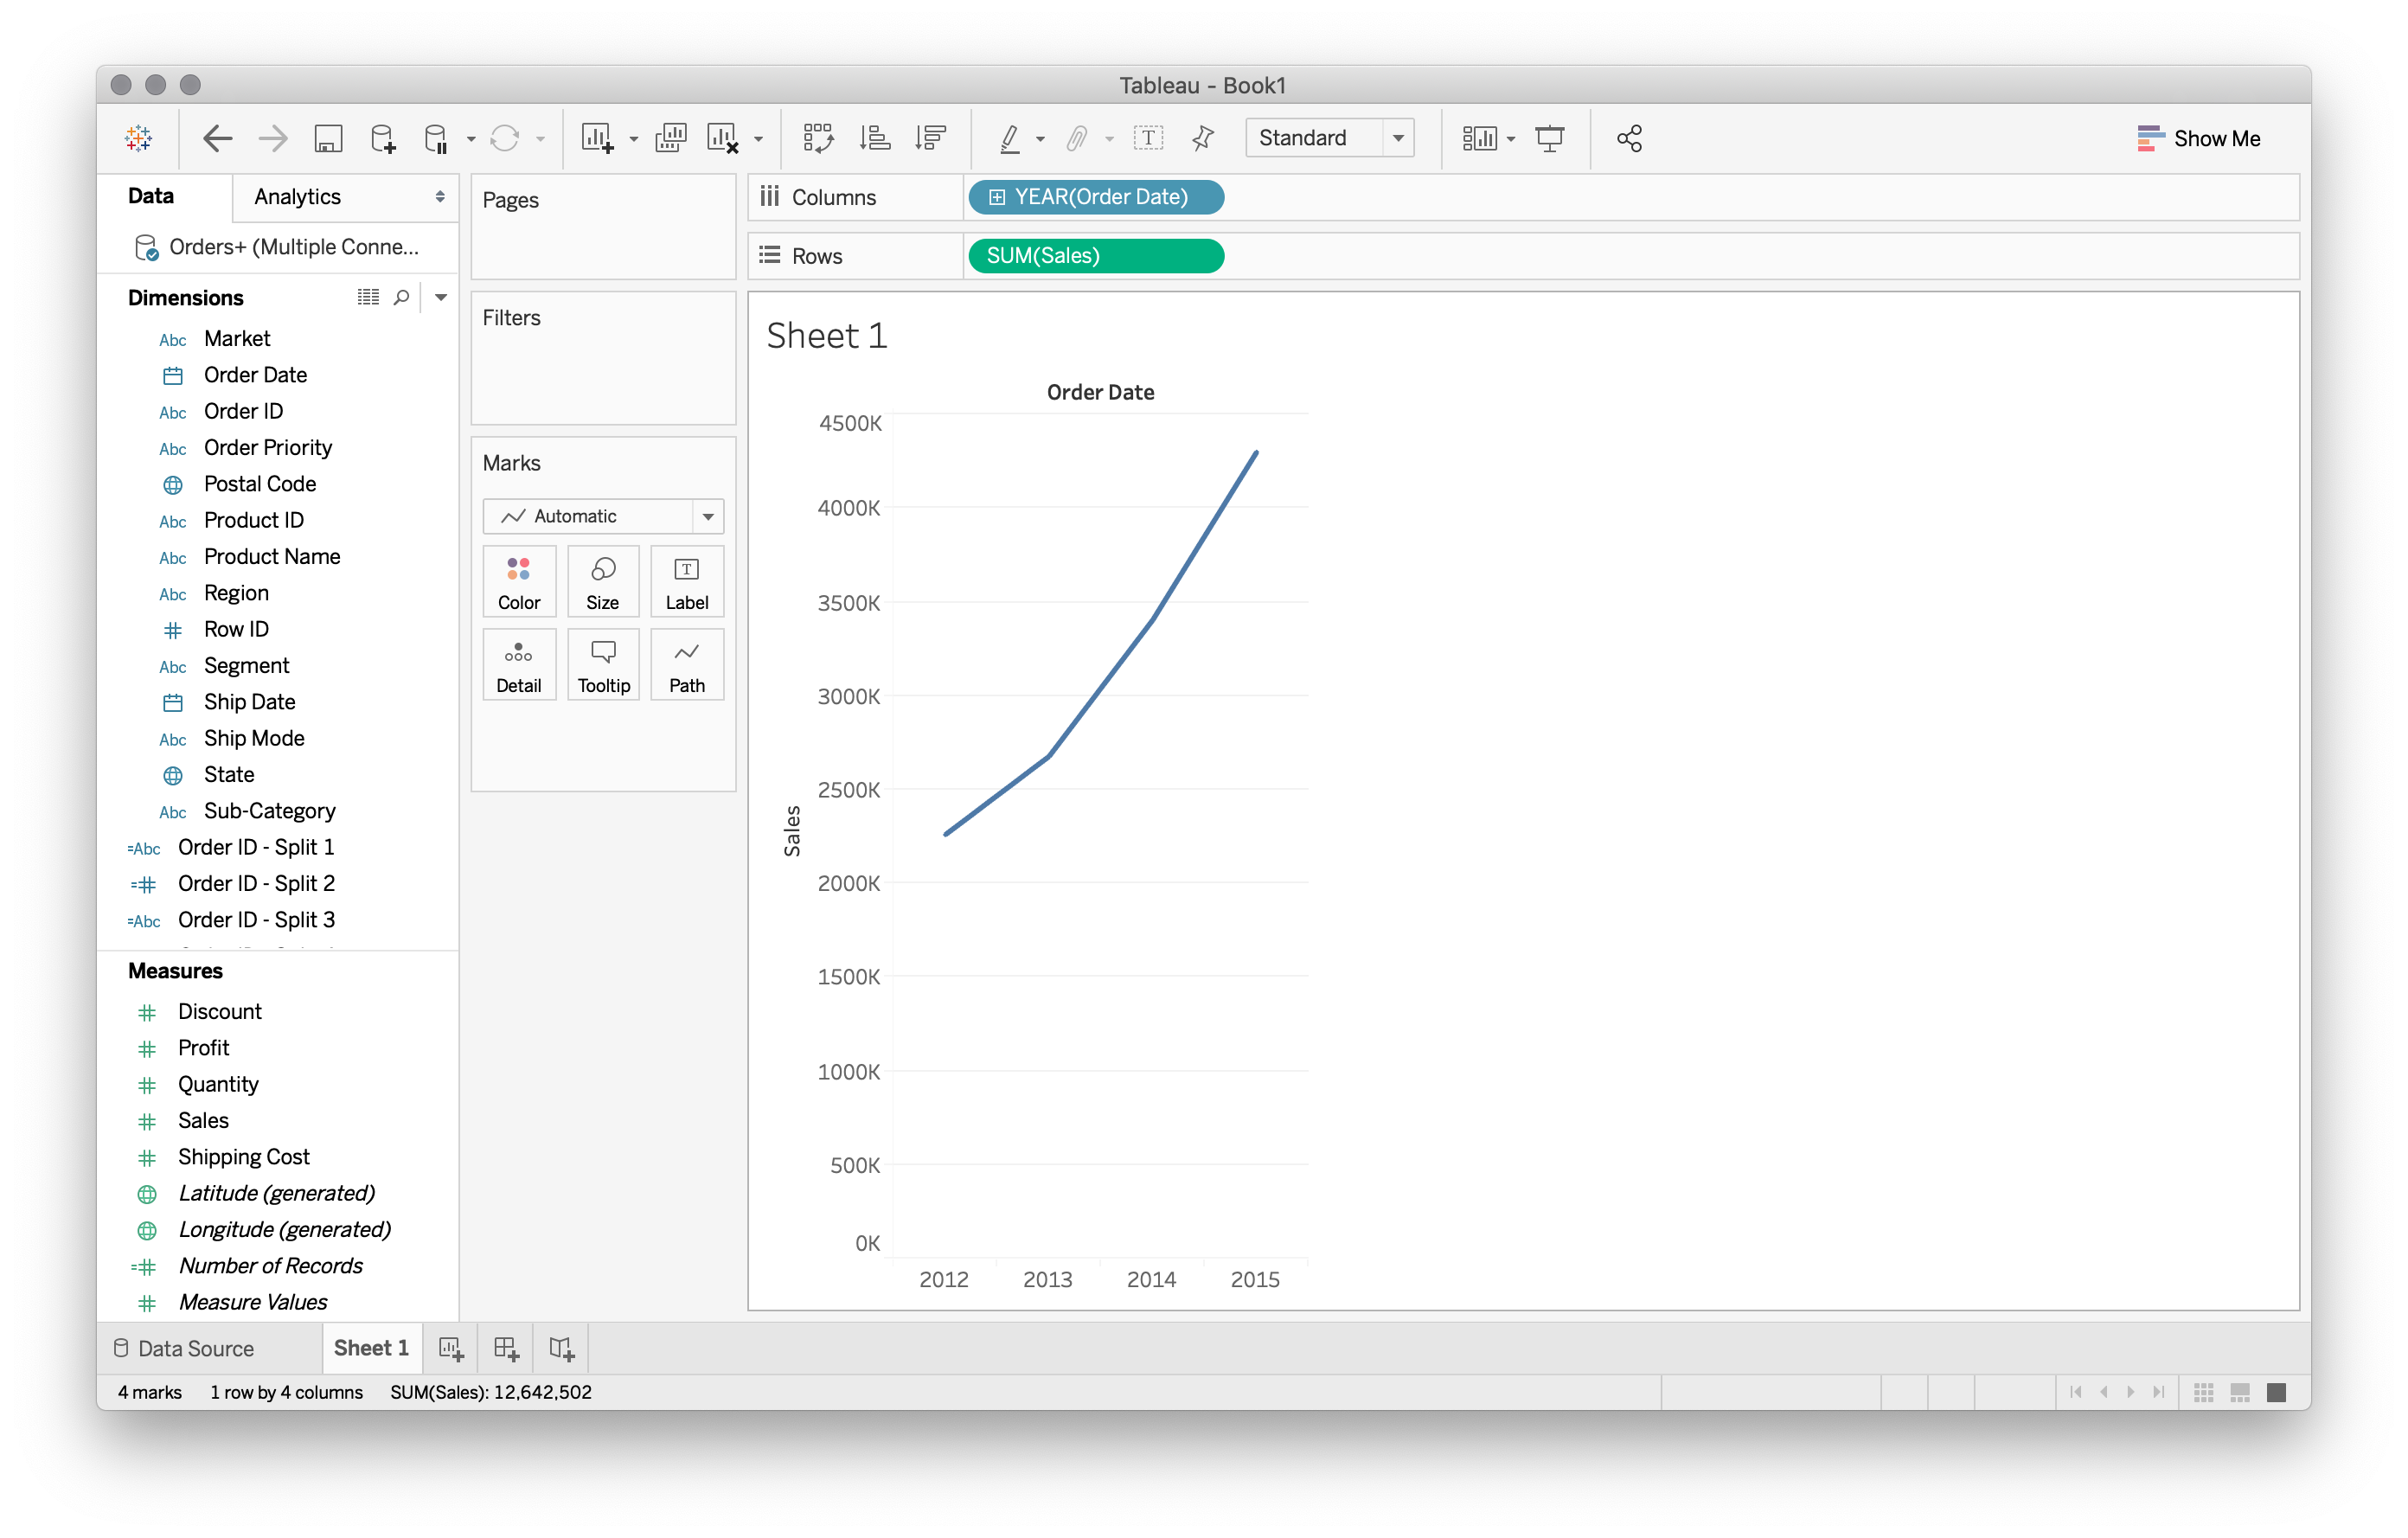
\includegraphics[width=1.05\textwidth]{img/sales}
\end{center}
\end{frame}


\begin{frame}
\begin{itemize}
\item  Notice how Tableau will guess at useful aggregations of our data.  
\vfill
\item We can change these fields by clicking the pills located on each shelf 
\begin{itemize}
\item eg.  change SUM to MEDIAN by Measure (Sum) $>$ Median .
\item eg.  change the sales per year to sales per quarter or sales per month (see next slide for details)
\end{itemize}
\end{itemize}

\end{frame}



\begin{frame}
For example, we may want to see \textit{average} sales month-to-month for each year. 
\begin{itemize}
\item Click the + sign to the Left of the blue pill, to granulate the dates into finer subcategories (ie. Quarters)\vfill 
\item Drag year to the right of Quarter so that we see each quarter yearly (rather than each year quarterly)\vfill
\item Then drag year to `Color' to change this side by side line graph to a single line graph with a legend.\vfill
\item Change Quarter to Month to get the next level of granularity for these dates \vfill
\item  Click the downarrow on the green pill and change Measure (Sum) > Average.
\end{itemize}


\end{frame}

\begin{frame}
\begin{center}
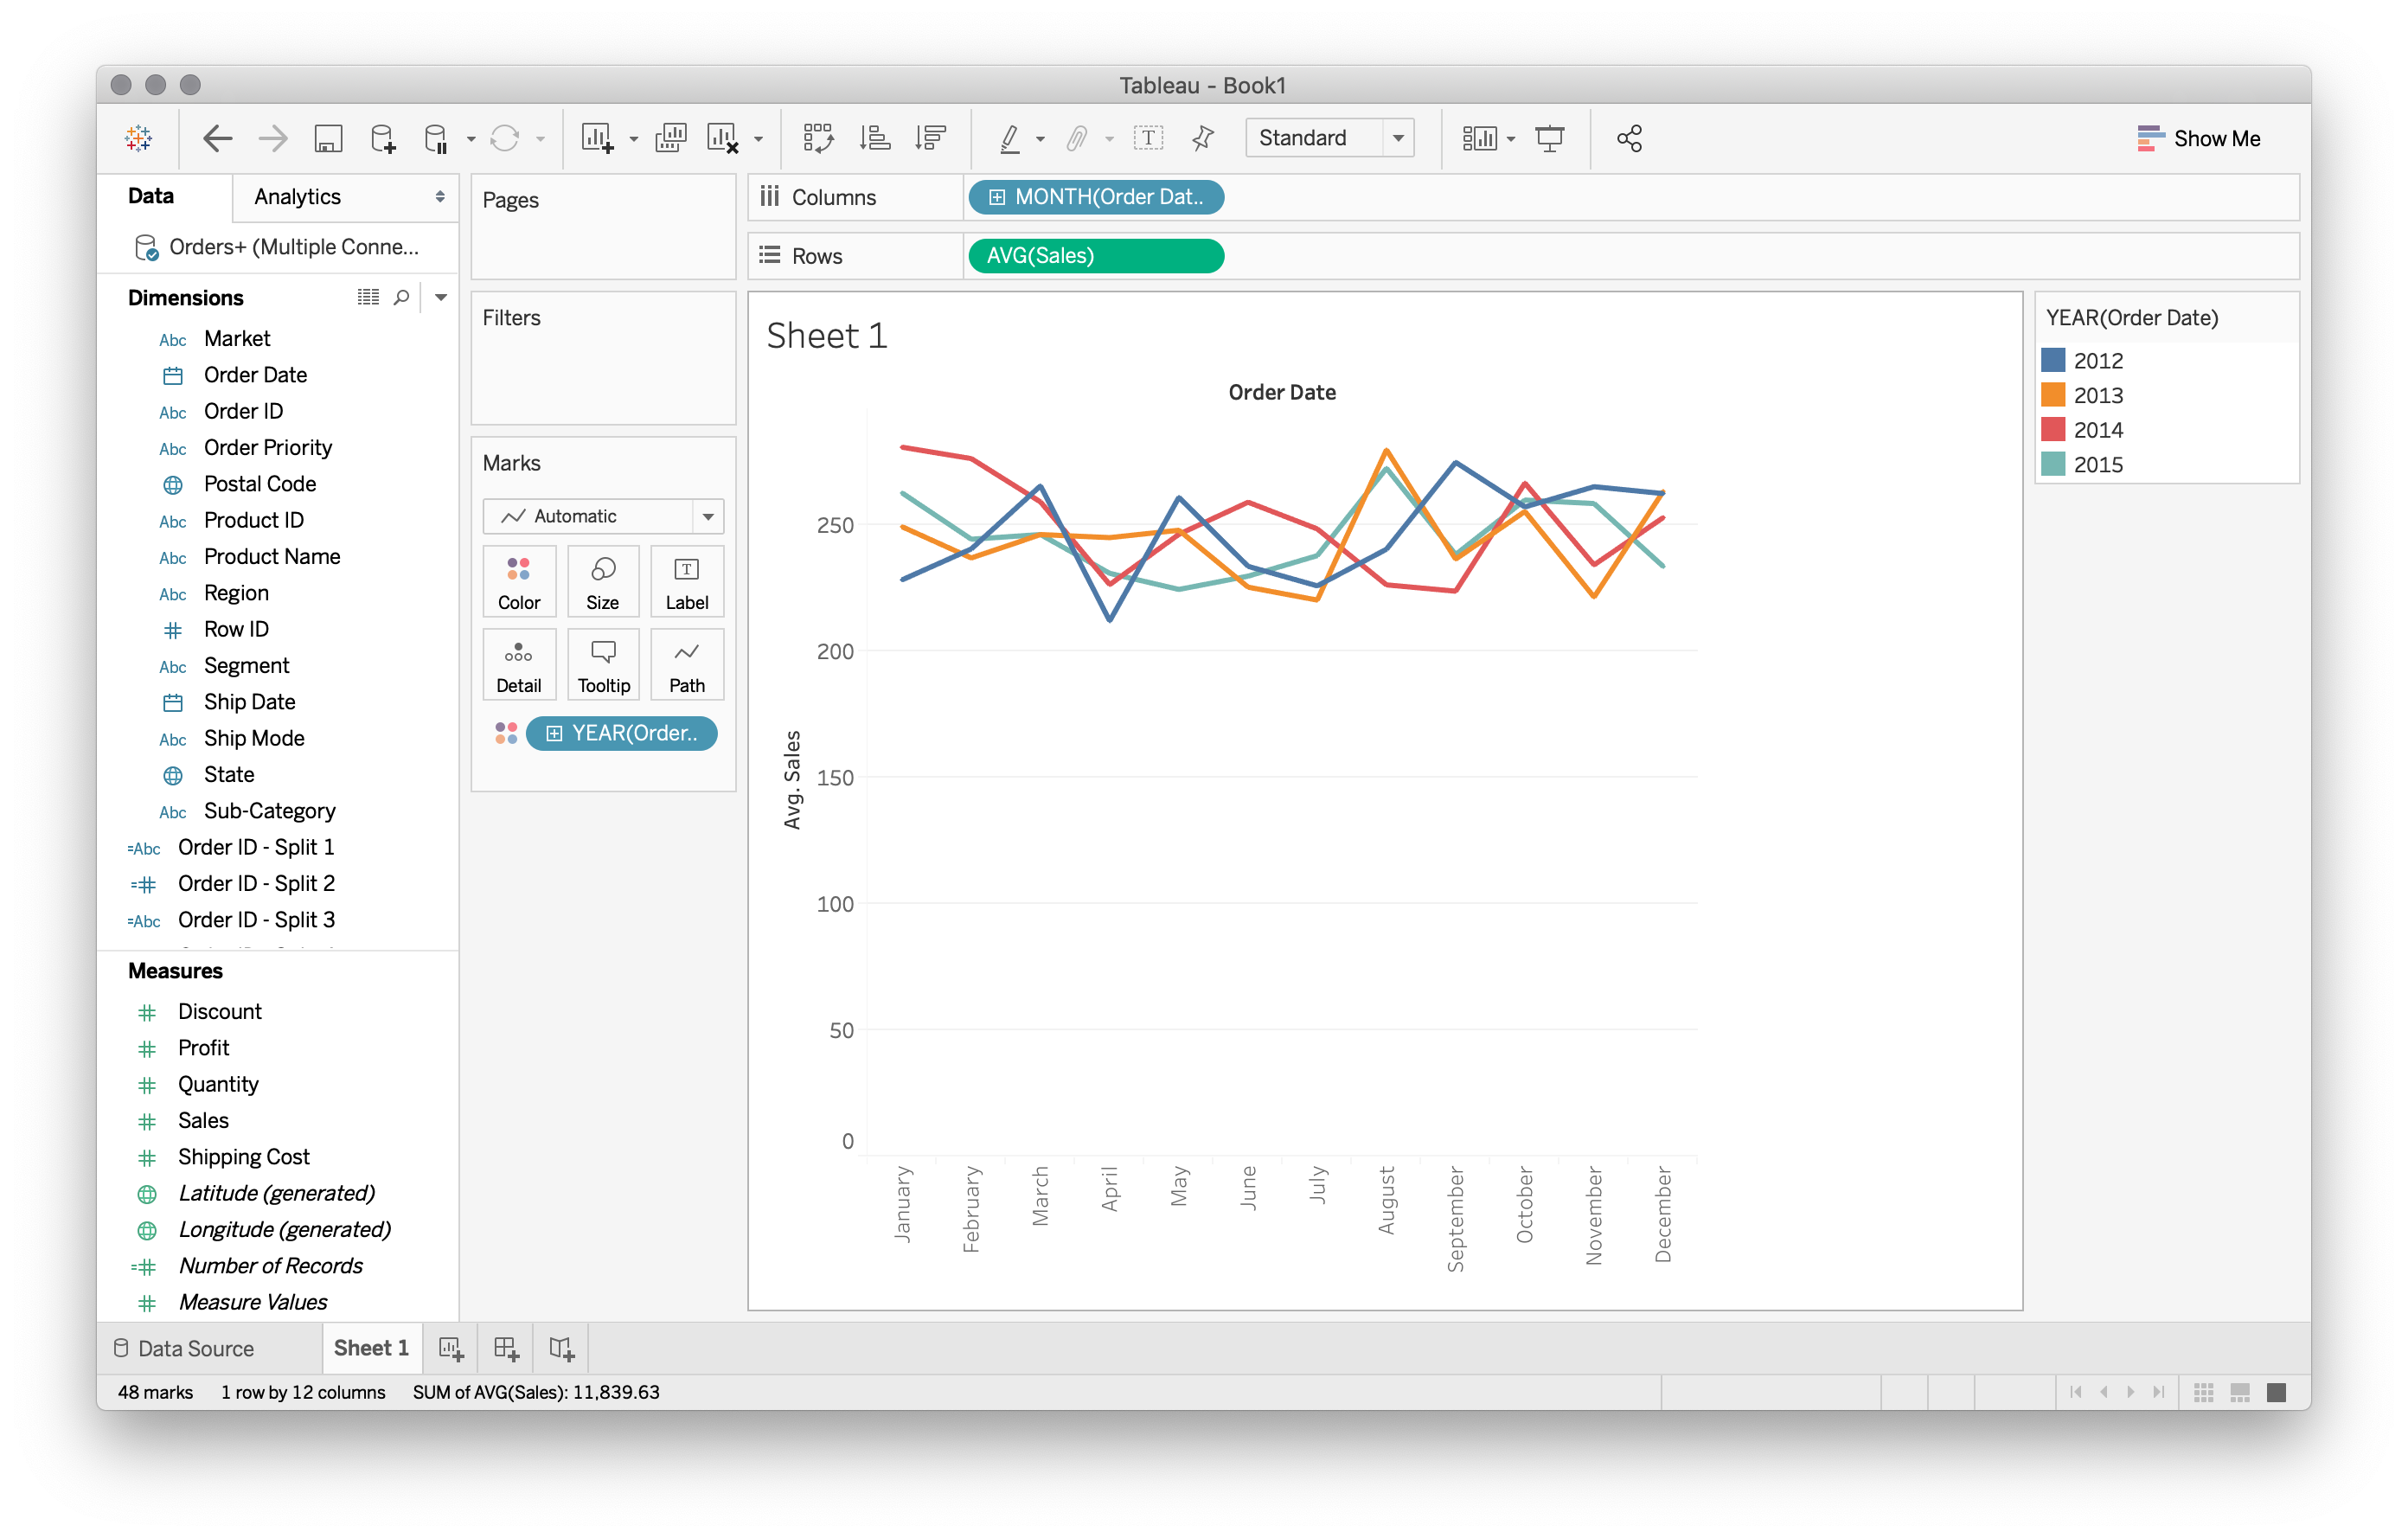
\includegraphics[width=1.05\textwidth]{img/sales2}
\end{center}

\end{frame}

\begin{frame}
There are a number of other `quick calculations' we have to choose from:
\begin{center}
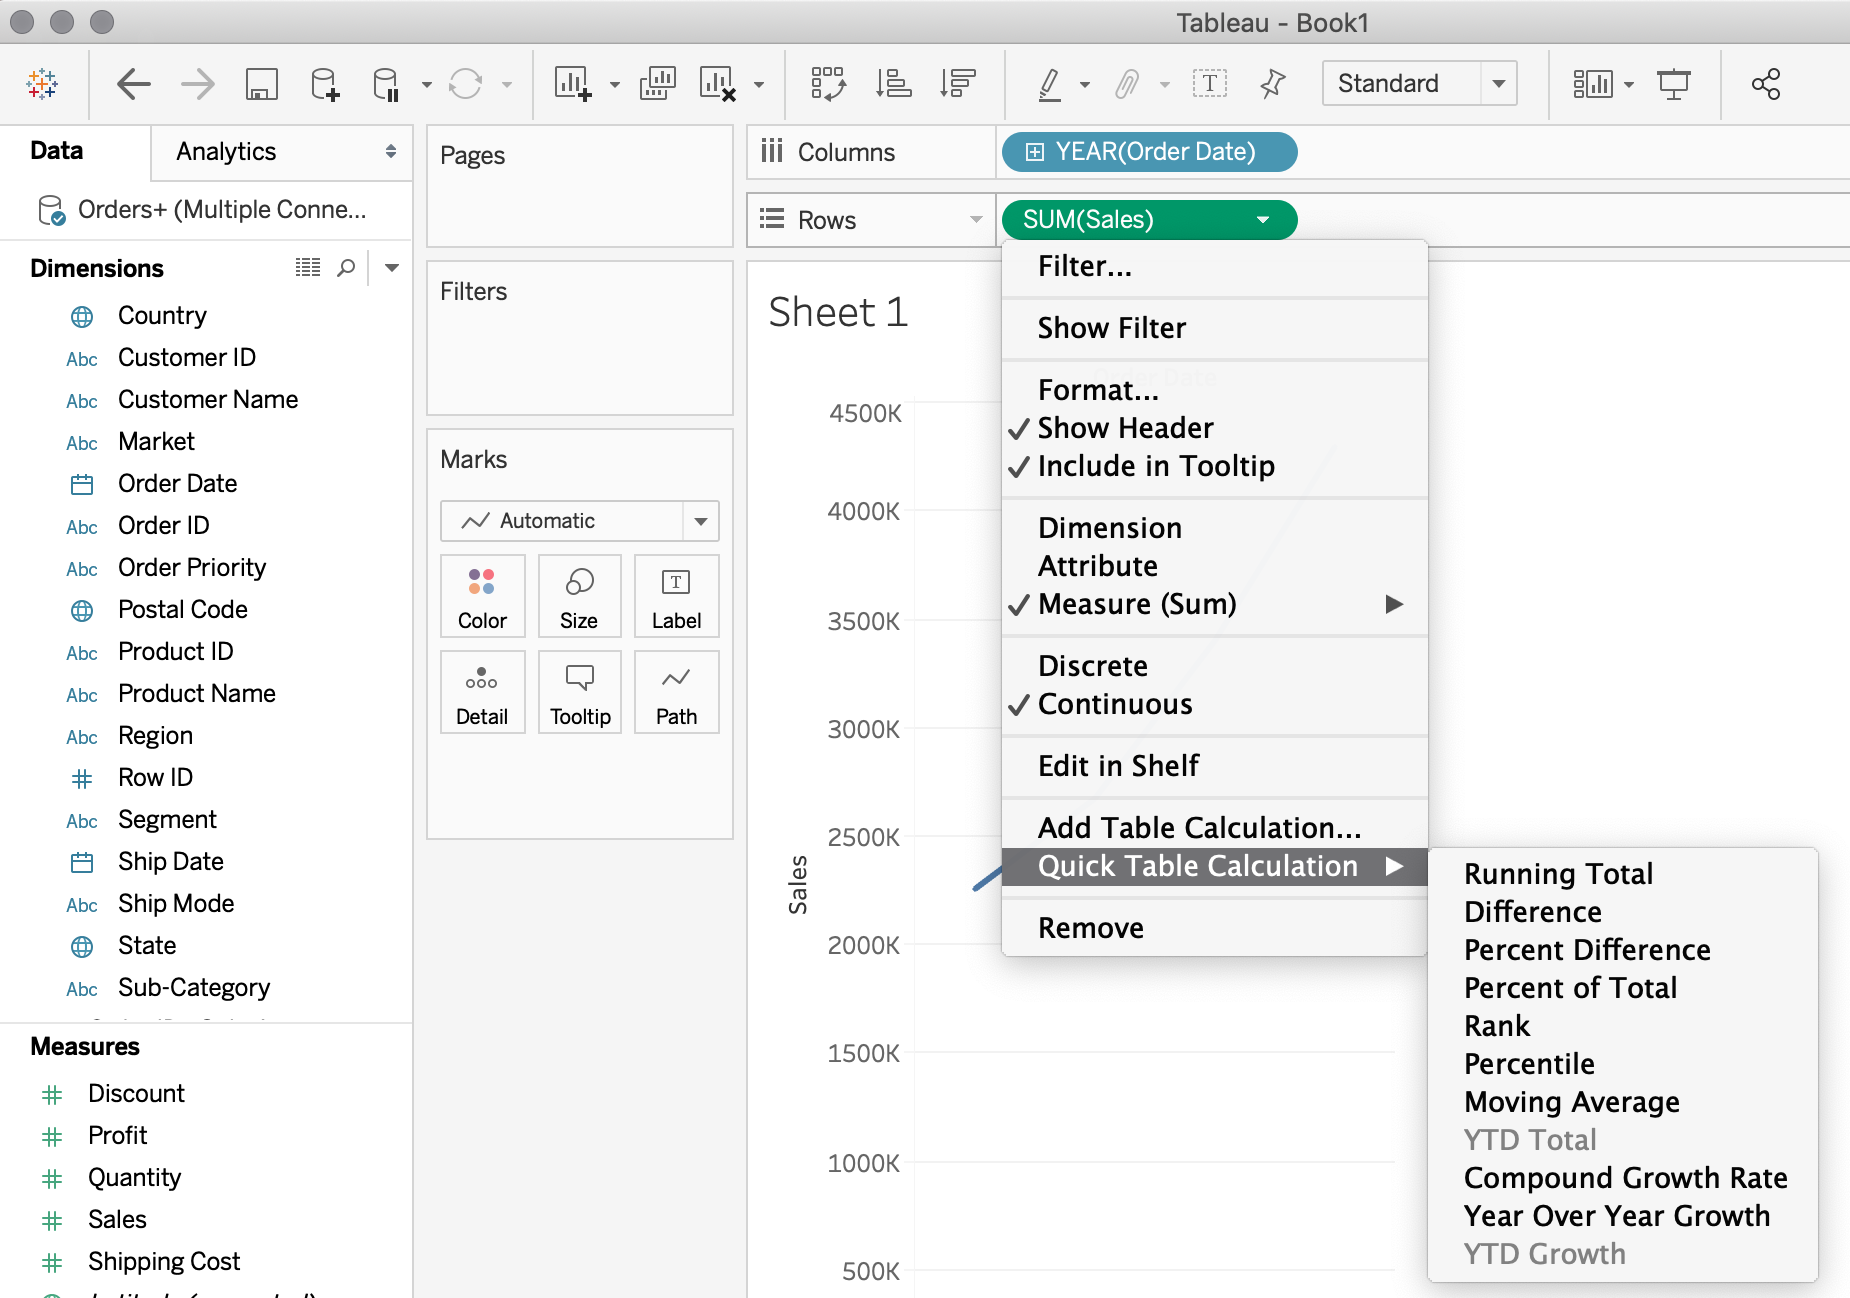
\includegraphics[width=.85\textwidth]{img/quickCalcs}
\end{center}

\end{frame}


\begin{frame}[fragile]\ft{Show Me Button}

\begin{itemize}
\item The \emph{Show Me} button suggests visualization to use based on your current dimensions and measures.\vfill

\item Choose the desired dimensions and measures by selecting them with your cursor while holding down the {Ctrl} key (window) or Cmnd key (mac).\vfill

\item As your selections change, different chart types will be suggested for you (i.e. they will become highlighted) .\vfill

\item Think of Show Me as your one-click option that will automatically place pills on shelves.
\end{itemize}
\end{frame}


\begin{frame}
Eg, since Country has a geographical component, a map seems like a natural choice:
\ft{Show Me}
\begin{center}
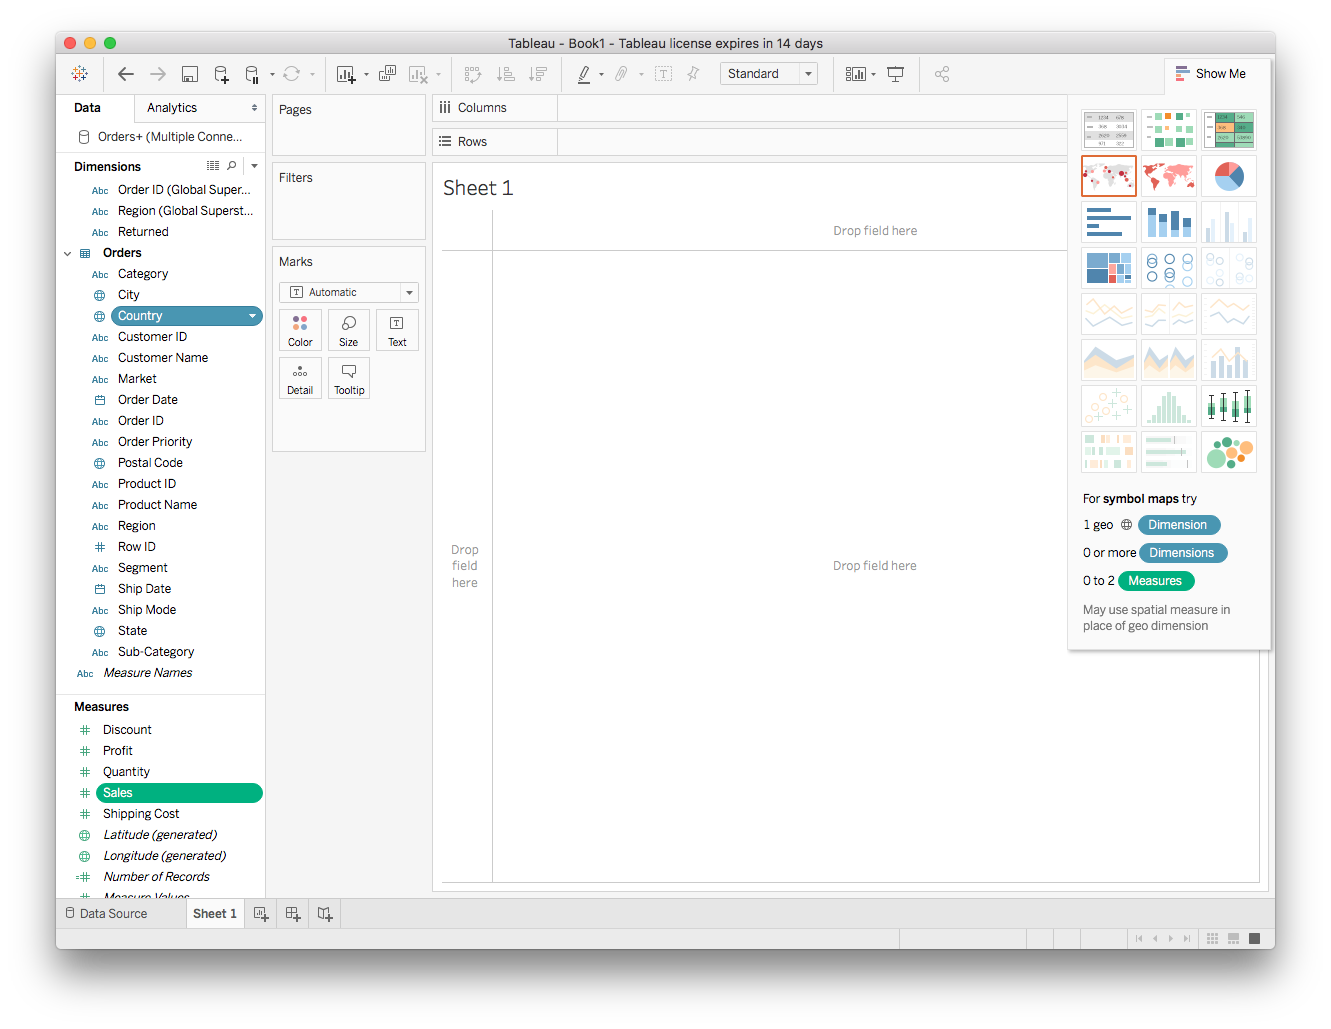
\includegraphics[width=.95\textwidth]{img/showme}
\end{center}
\end{frame}

\begin{frame}\ft{Show Me}
For geographic data (small globe icon), Tableau automatically generates center-point geocodes (longitude/latitude).
\begin{center}
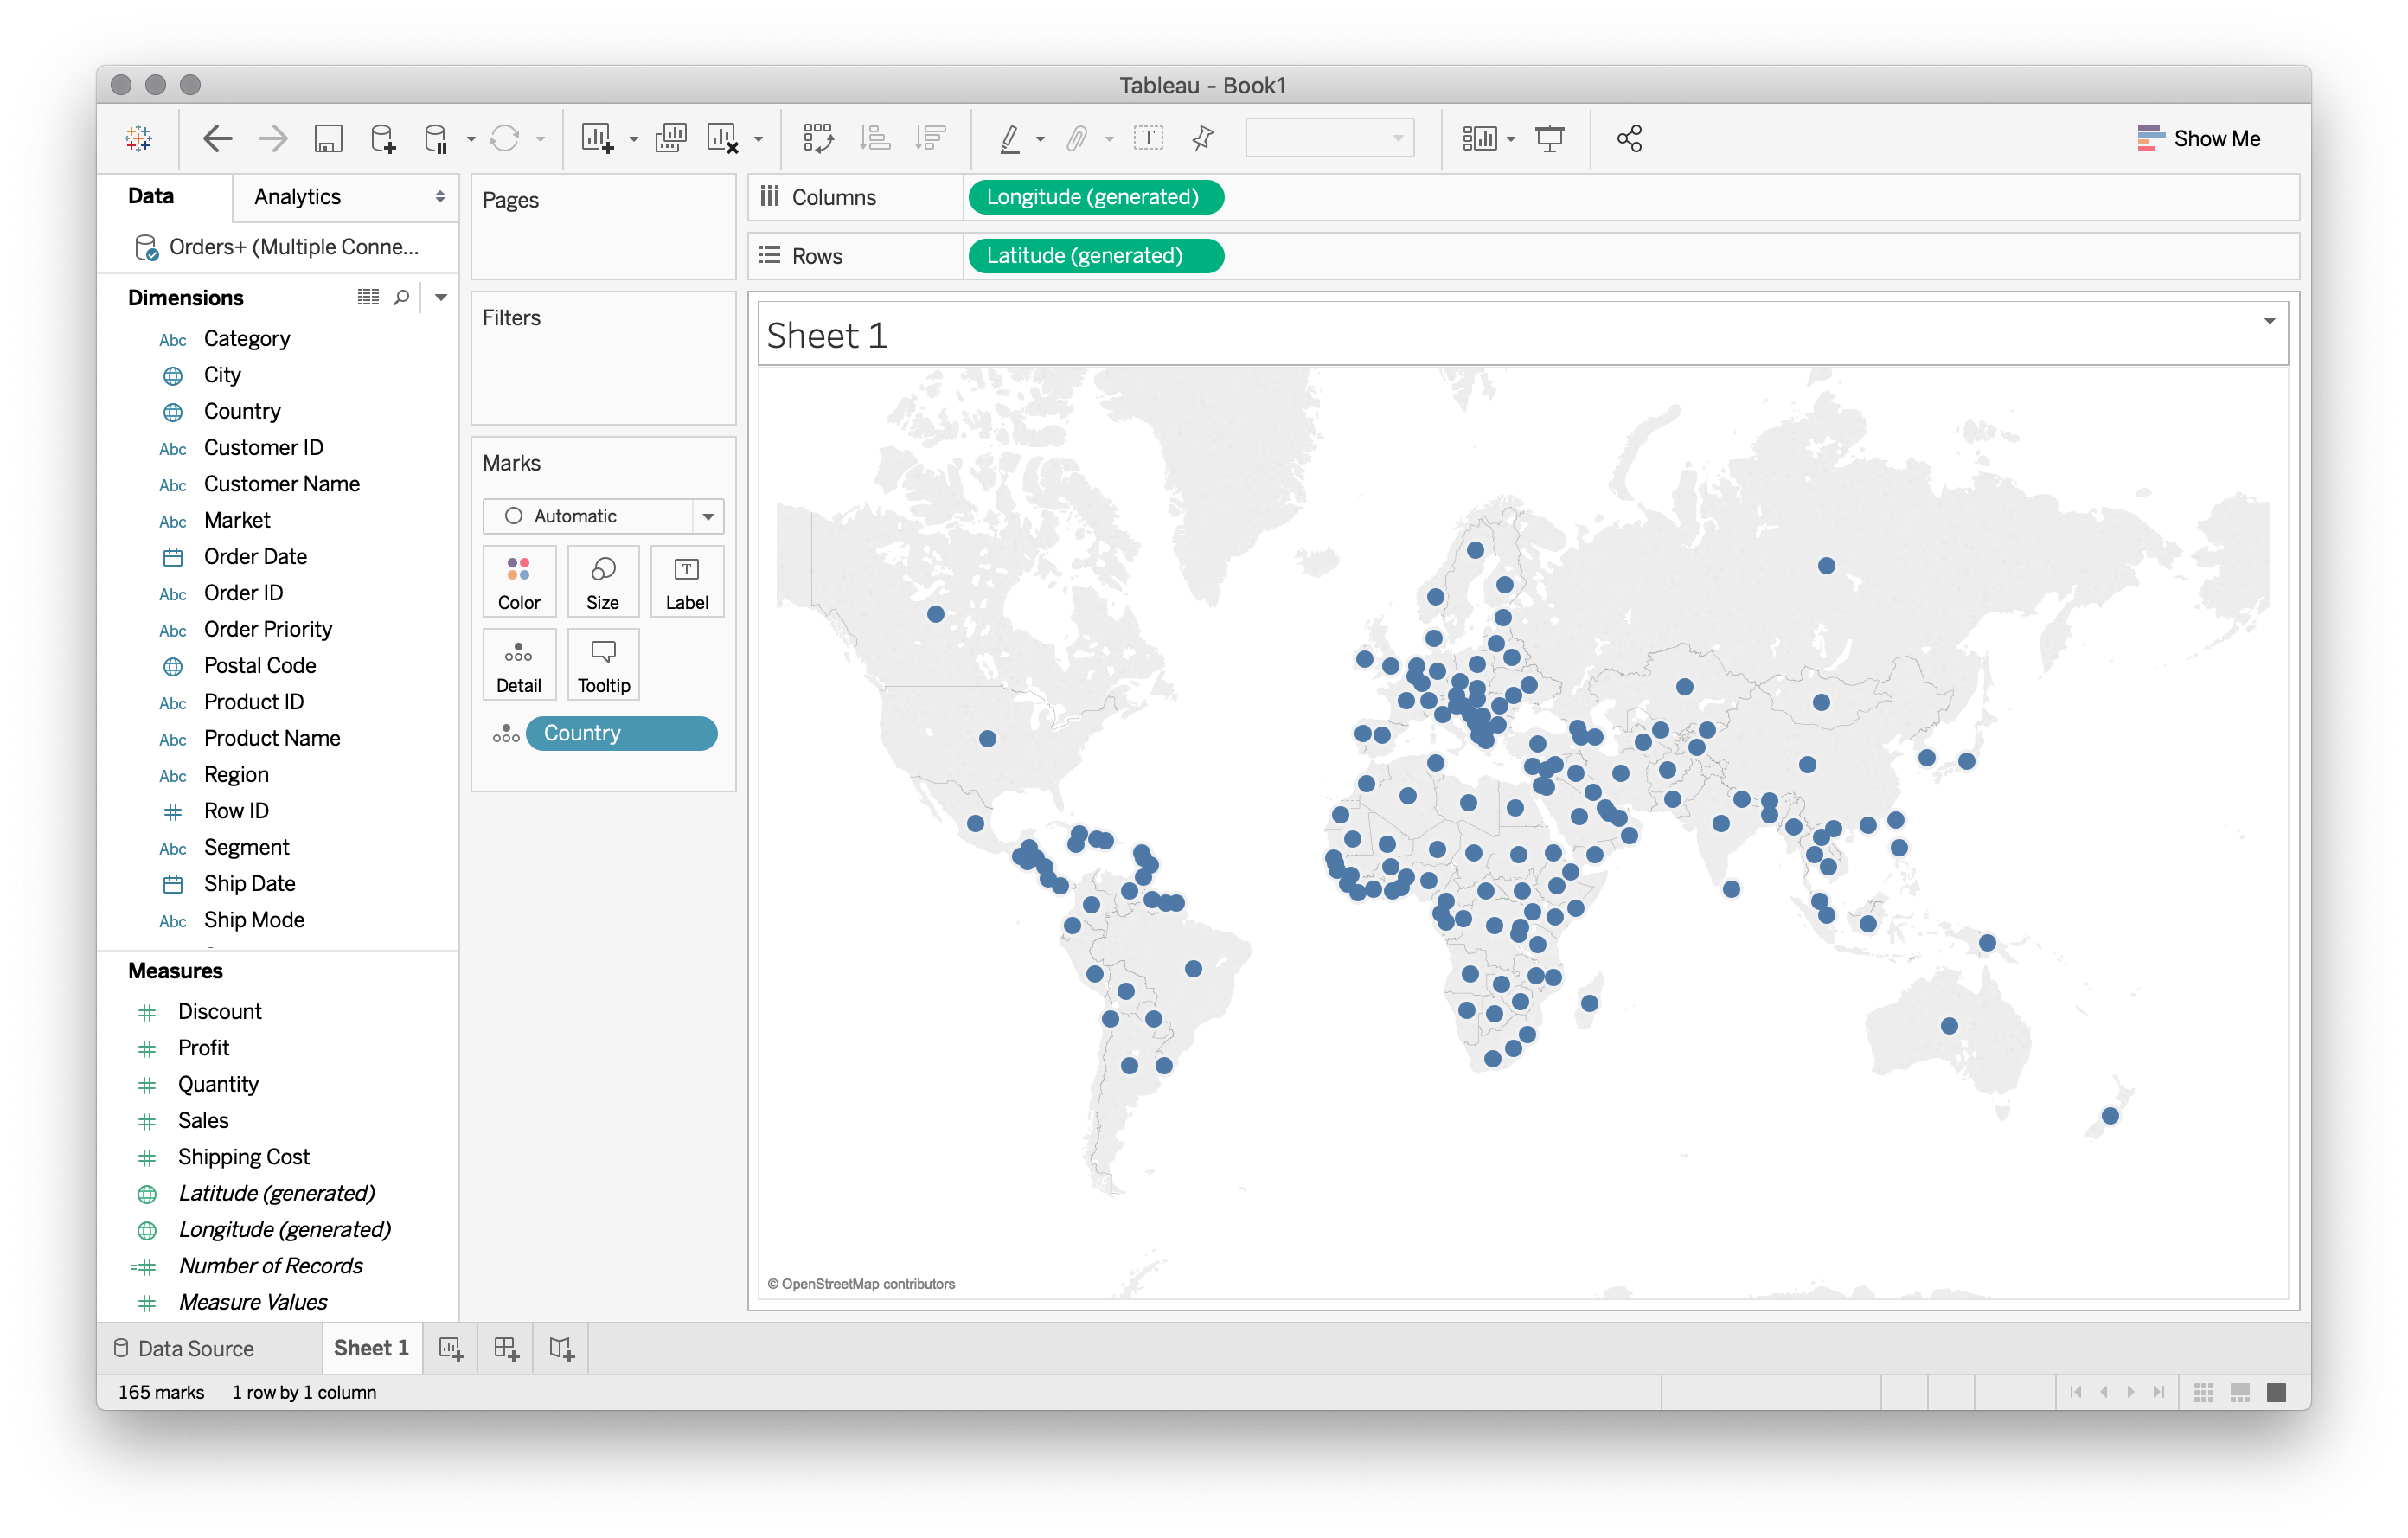
\includegraphics[width=.95\textwidth]{img/map}
\end{center}
\end{frame}


%\begin{frame}\ft{Geographic Data}
%\begin{itemize}
%\item For geographic data (small globe icon), Tableau automatically generates center-point geocodes (longitude/latitude).
%\end{itemize}
%\end{frame}


\begin{frame}\ft{Show Me}
We can click and drag `Sales' onto the map to include this information in the graphic (depicted by size of the dot, also visible when hovering over the country)
\begin{center}
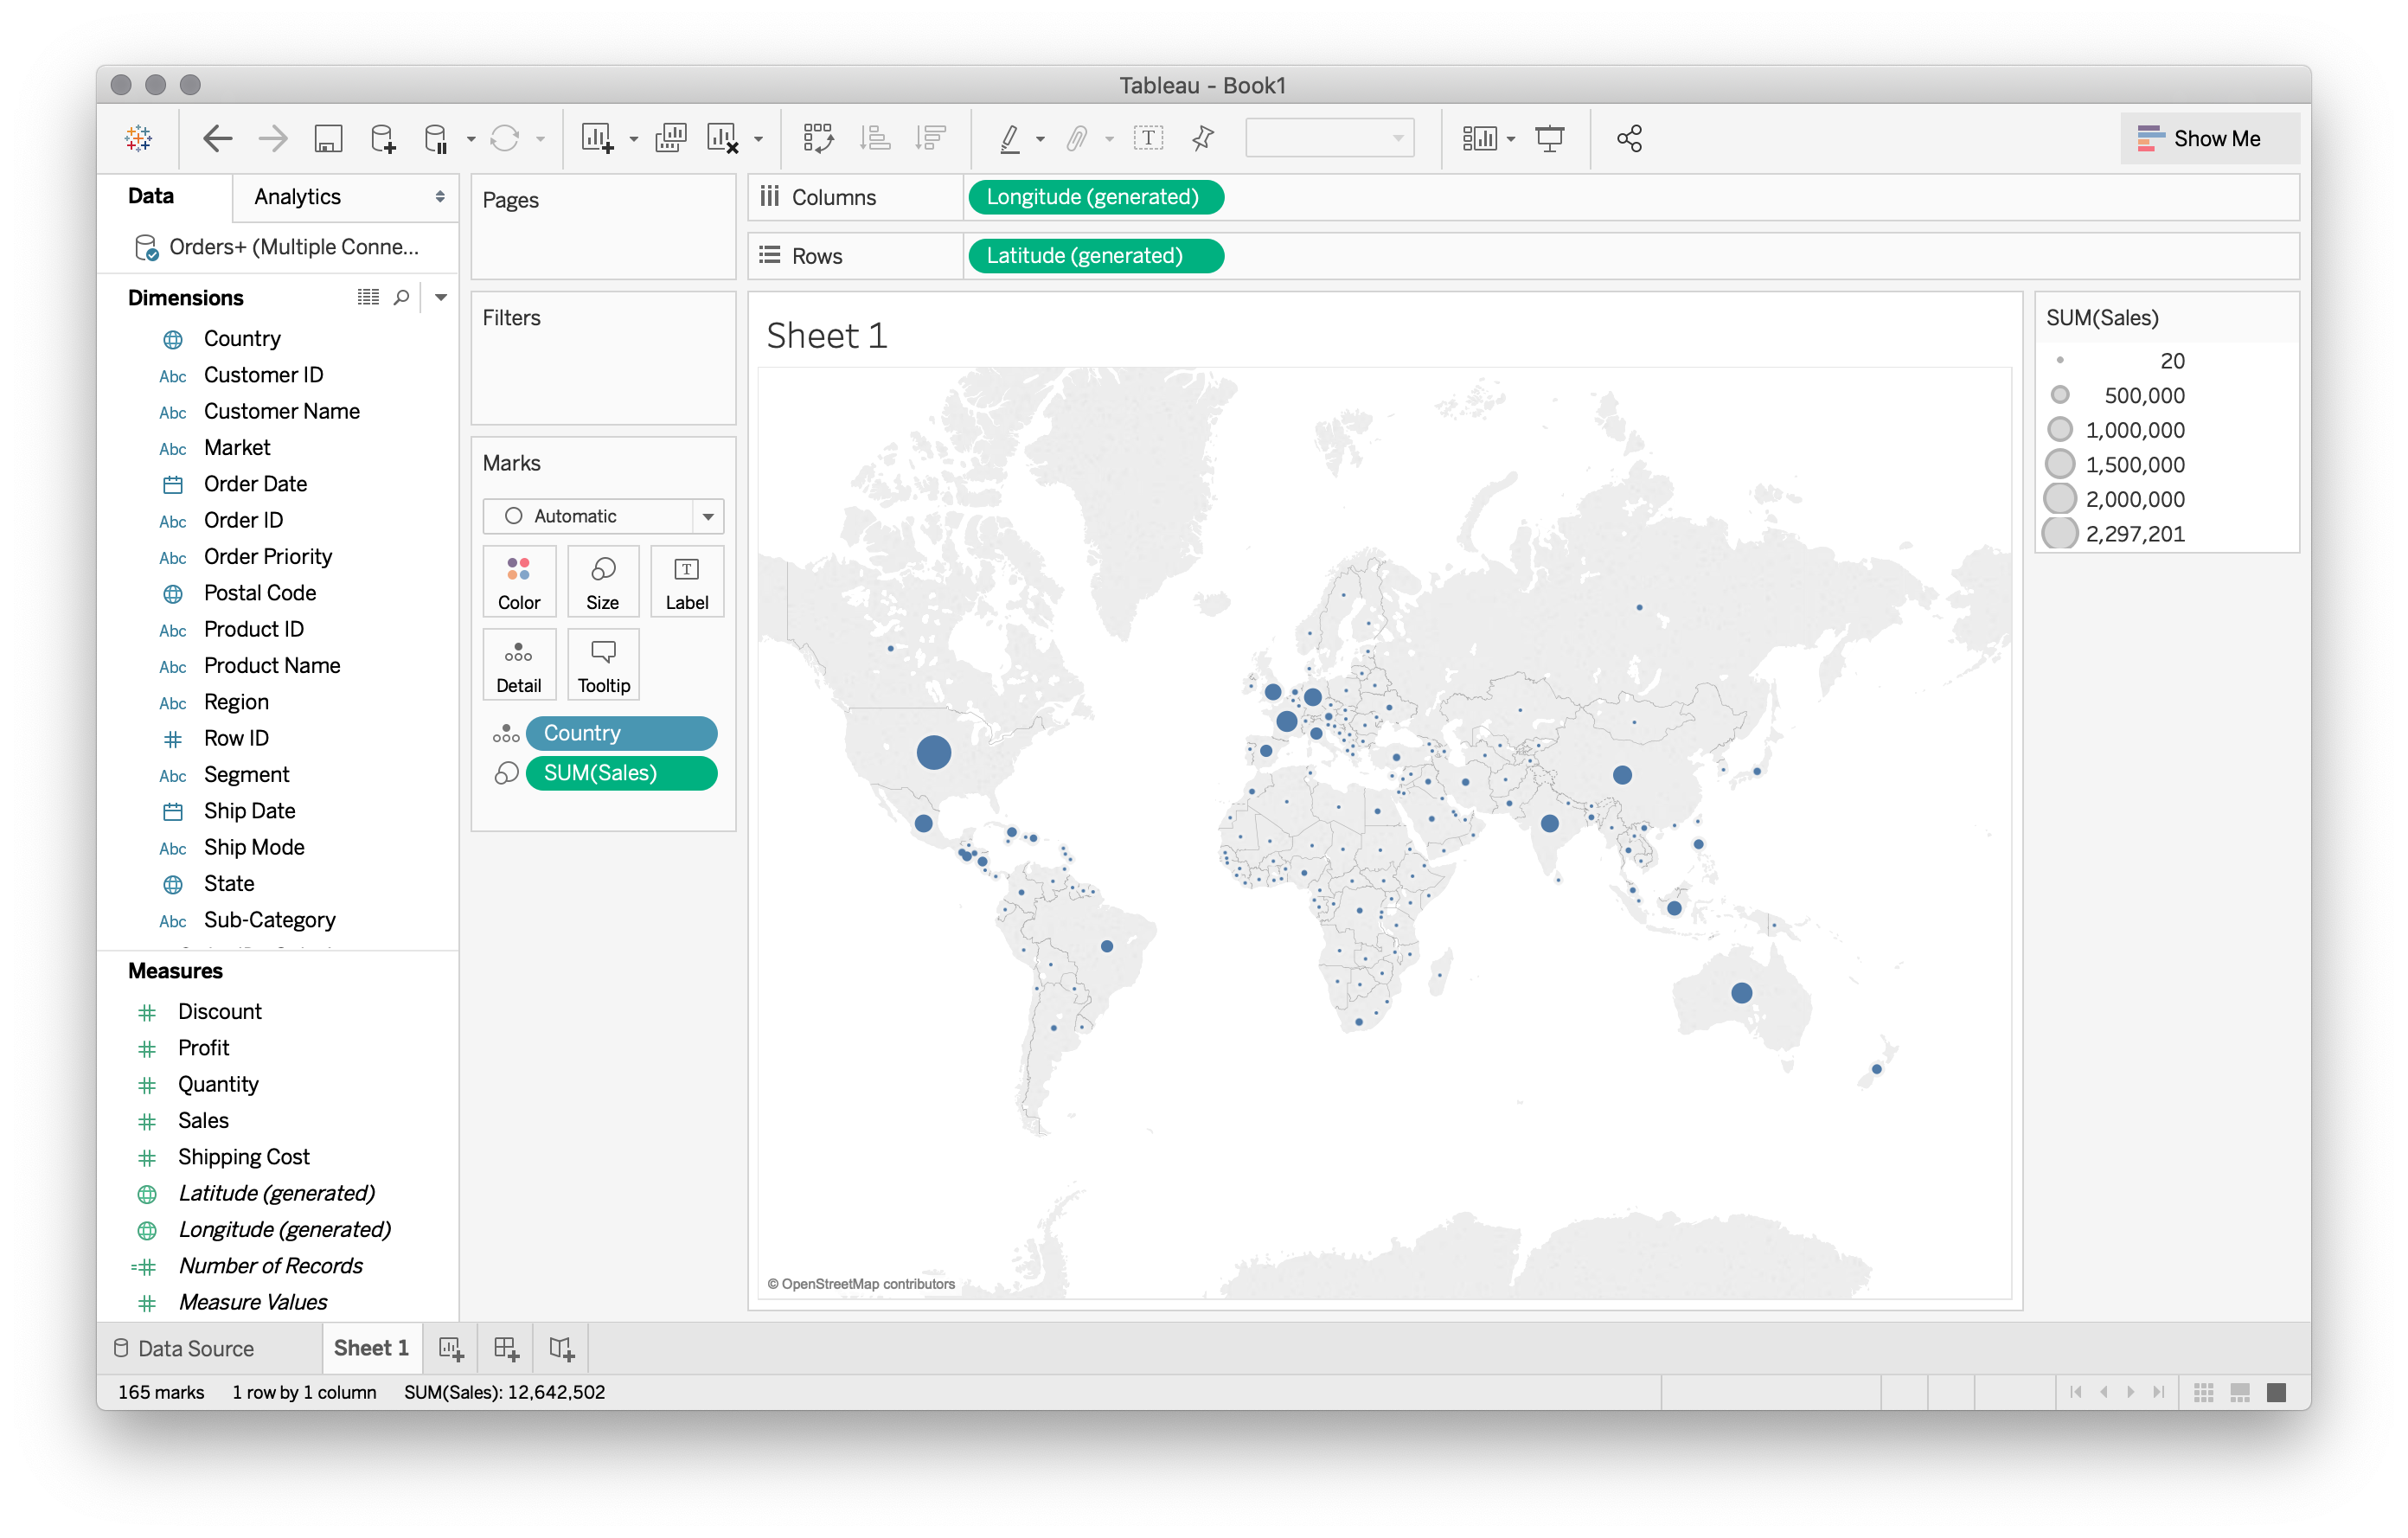
\includegraphics[width=.95\textwidth]{img/sales3}
\end{center}
\end{frame}




\begin{frame}\ft{Tableau Question}
\begin{example}
How many of the following statements are TRUE?
\begin{enumerate}
\item In Tableau blue pills are continuous. 
%\item The View Cards interface allows for changing color and size of features in the visualization. 
\item A shelf is a location to place a pill.
\item The Show Me button will suggest visualizations for you.
\item A pill for a dimension may be on more than one shelf at the same time.
\end{enumerate}
\begin{multicols}{5}
\begin{enumerate}[A)]
\item 0 
\item 1
\item 2
\item 3
\item 4
\end{enumerate}
\end{multicols}
\end{example}
\end{frame}



\begin{frame}\ft{Tableau Question}
\begin{block}{Answer}
How many the following statements are TRUE?
\begin{enumerate}
\item In Tableau blue pills are continuous.\pxmark
%\item The View Cards interface allows for changing color and size of features in the visualization.  \pcmark
\item A shelf is a location to place a pill.  \pcmark
\item The Show Me button will suggest visualizations for you.  \pcmark
\item A pill for a dimension may be on more than one shelf at the same time.  \pcmark
\end{enumerate}
\begin{multicols}{5}
\begin{enumerate}[A)]
\item 0 
\item 1
\item 2
\item {\bf 3}
\item 4
\end{enumerate}
\end{multicols}
\end{block}
\end{frame}


\begin{frame}\ft{Try it: Tableau Visulations}
\begin{example}
\begin{itemize}
\item Install Tableau. Use trial version or \href{https://www.tableau.com/academic/students}{Tableau for students}
\item Start Tableau. Use the sample.twbx file or the Superstore example and explore the visualizations.
\item Try create any visualization of the data.
\end{itemize}
\end{example}
\end{frame}


\begin{frame}\ft{Tableau - Data Sources}
Tableau can connect to a wide variety of data sources including:
\begin{itemize}
\item Microsoft Excel and Access
\item Text files (txt, csv)
\item Relational databases (MySQL, SQL Server, Oracle, PostgreSQL)
\item NoSQL databases (MongoDB)
\item Parallel and analytical databases (Greenplum, Vertica, Teradata)
\item Other ODBC sources (note JDBC is not supported)
\end{itemize}



%A sample data ource called Superstore is available in the Tableau/defaults/Datasources directory.
%\begin{itemize}
%\item File: Sample - Superstore.tds (Tableau Data Source) or
%\item File: Sample - Superstore.xls (Excel file)
%\end{itemize}

\end{frame}




\begin{frame}
\ft{Connecting to relational databases}
Connecting to a relational database like MySQL  and Microsoft SQL requires:
\begin{itemize}
\item Driver (often need to \href{https://www.tableau.com/support/drivers}{download} from database vendor) %\href{https://www.tableau.com/en-us/support/drivers?edition=pro&lang=en-us&platform=mac&cpu=64&version=2018.3&__full-version=20183.18.1018.1932#mysql}{MySQL driver}
\item Database connection information %(password: ubc)
\end{itemize}
\end{frame}




\begin{frame}
\ft{Connecting to relational databases}
Once you have the necessary driver, you simple click on the appropriate option on the left hand panel of the home screen:
\begin{center}

\includegraphics[width=.85\textwidth]{img/sql}
\end{center}
\end{frame}


\begin{frame}
\ft{Connecting to relational databases}
At this point you will be asked to fill in the required fields in a pop a window like this:
\begin{center}
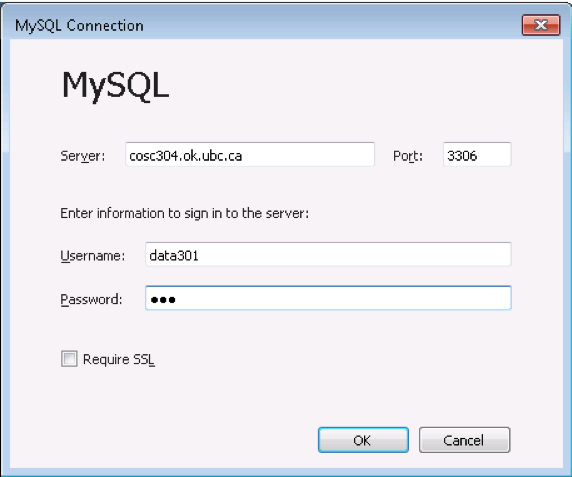
\includegraphics[width=.5\textwidth]{img/mysql}
%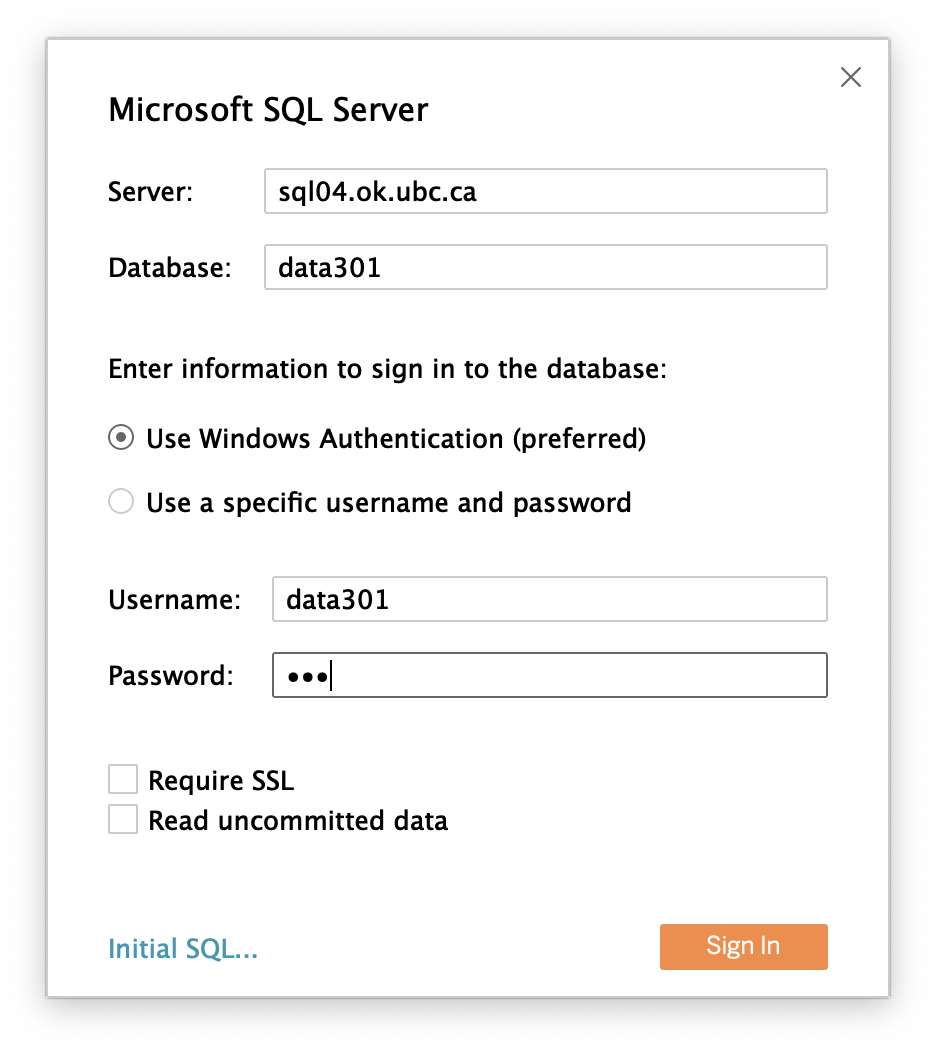
\includegraphics[width=.5\textwidth]{img/microSQL}
\end{center}
Using the above credentials with password {\tt ubc} should grant you access to the {\tt WorksOn} database that we have studied in out SQL unit.
\end{frame}

\begin{frame}
In order to connect to this database you need to be on {\bf ubcsecure} wifi \textit{on campus}. 
\vfill
To access it from home:
\begin{itemize}
\item Download VPN tool at: https://myvpn.ok.ubc.ca/ and follow instructions there.
\item Launch Cisco AnyConnect and enter myvpn.ok.ubc.ca as the host and click Connect.
\item Enter CWL to authenticate.
\end{itemize}

\end{frame}




\begin{frame}
\ft{Connecting to MySQL}
\begin{center}
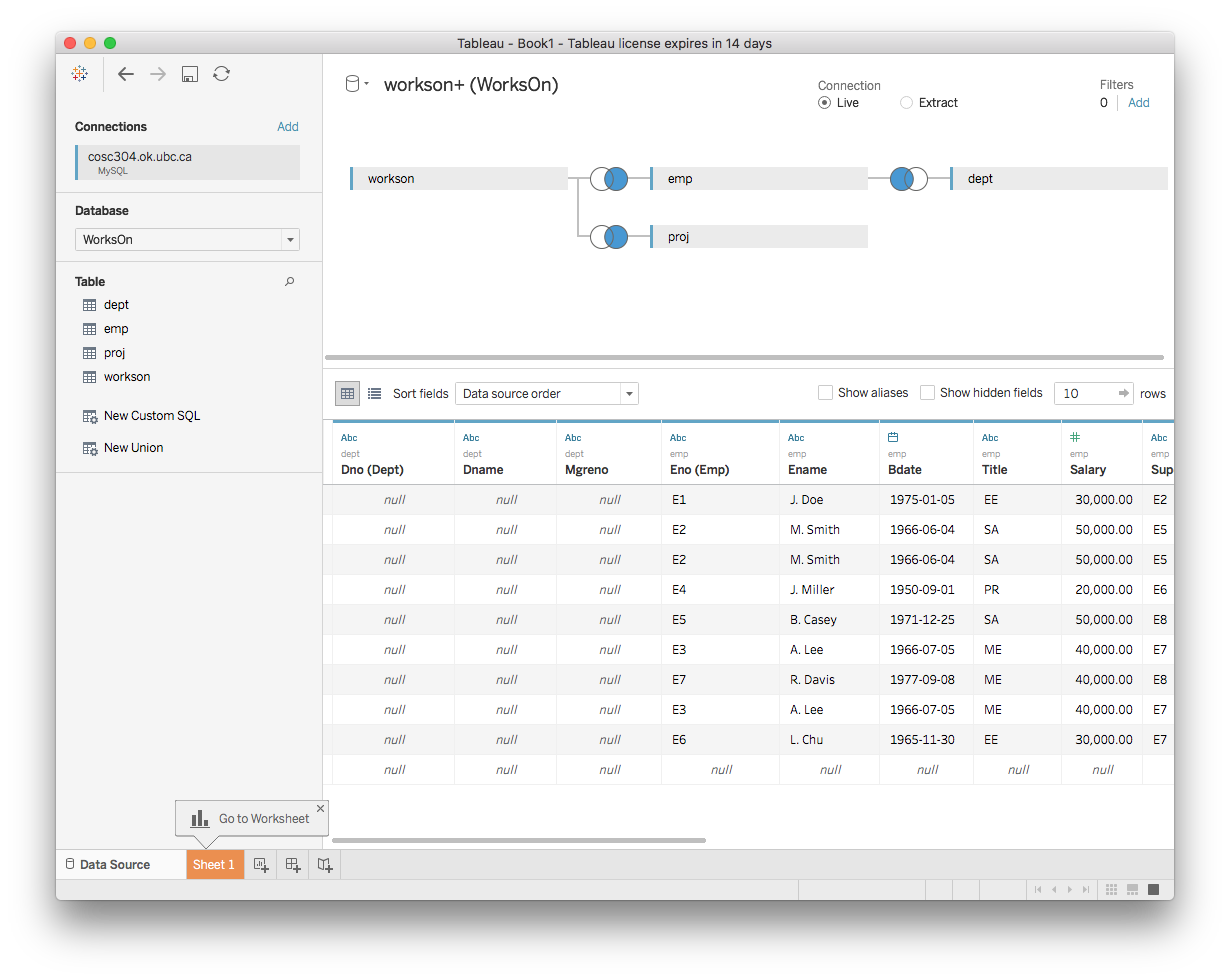
\includegraphics[width=.9\textwidth]{img/mySQLtables}
\end{center}
\end{frame}



\begin{frame}\ft{Connect or Extract Data}
Tableau has its own internal data engine. There are two options when retrieving data to visualize:
\begin{enumerate}
\item Direct connect to source to get live data
\begin{itemize}
\item Can refresh data using F5 or selecting refresh menu item
\item May be faster depending on data set/visualization
\end{itemize}
\item  Extract and import data into Tableau's data engine
\begin{itemize}
\item May get a performance improvement as data is local
\item May set certain scheduled times to extract and keep data up to date
\item Portability (as consumer of report does not need access to data source)
%\item Support for functions not supported by source (e.g. Excel)
\end{itemize}
\end{enumerate}
\end{frame}



\begin{frame}\ft{Tableau Data Source Question}
\begin{example}
How many of the following statements are TRUE?
\begin{enumerate}
\item Tableau can connect to  relational databases.
\item  Tableau can process data in text and Excel files.
%\item  Tableau can either leave data in data source or extract it locally.
\item  Tableau can JOIN information across tables from multiple sources.
%\item Tableau can connect to data sources using JDBC.
\item  Tableau will try to identify types and relationships from the data sources.
\end{enumerate}
\begin{multicols}{5}
\begin{enumerate}[A)]
\item 0 
\item 1
\item 2
\item 3
\item 4
\end{enumerate}
\end{multicols}

\end{example}
\end{frame}



\begin{frame}\ft{Tableau Data Source Question}
\begin{block}{Answer}
How many of the following statements are TRUE?
\begin{enumerate}
\item Tableau can connect to  relational databases. \pcmark
\item  Tableau can process data in text and Excel files.\pcmark
%\item  Tableau can either leave data in data source or extract it locally.\pcmark
\item  Tableau can JOIN information across tables from multiple sources.\pcmark
%\item Tableau can connect to data sources using JDBC.\pxmark
\item  Tableau will try to identify types and relationships from the data sources.\pcmark
\end{enumerate}
\begin{multicols}{5}
\begin{enumerate}[A)]
\item 0 
\item 1
\item 2
\item 3
\item {\bf 4}
\end{enumerate}
\end{multicols}

\end{block}
\end{frame}



\begin{frame}\ft{Try it: Tableau Data Sources}
\begin{example}
Use Tableau to connect to Excel and MySQL data sources.
\begin{itemize}
\item Start Tableau. Open up Superstore Excel data source (either XLS or TDS file) in Tableau/defaults/Datasources directory.
\item \href{https://dev.mysql.com/downloads/connector/odbc/}{install} the MySQL ODBC connector
\item  Server: cosc304.ok.ubc.ca  Database: data301  User: data301  Password: ubc
\end{itemize}

Superstore visualizations:
\begin{itemize}
\item Map showing profit by state. Save this sheet as {\tt State Profit}
\item Visualization to indicate what is the best selling product category per market. Save this sheet as {\tt Best Product}
\item Annotate the best selling product category for each market.
\end{itemize}
\end{example}

%WorksOn visualizations:
%\begin{itemize}
%\item Visualize the number of projects, employees, and hours worked per department.
%\item Visualize employee ages to see if age impacts if they are supervisors.
%\end{itemize}
\end{frame}

\begin{frame}\ft{Some notes}
\begin{itemize}
\item You can rename the tabs in Tableau in the same way we would in Excel (double click the the tab and rename).\vfill
\item If we want the raw data associated with a visualization, it is as simple as right clicking on the image, then selecting {\bf Copy} > {\bf Data} and pasting this information into Excel.\vfill
\item Alternatively, you could %right click on the tab and select `Duplicate as Crosstab', which will open our table into a new tab in Tableau.
go to toolbar and select {\bf Worksheet} $>$ {\bf Duplicate as Crosstab}.
\end{itemize}

\end{frame}


\begin{frame}
\ft{Copy data in Tableau}
\begin{center}
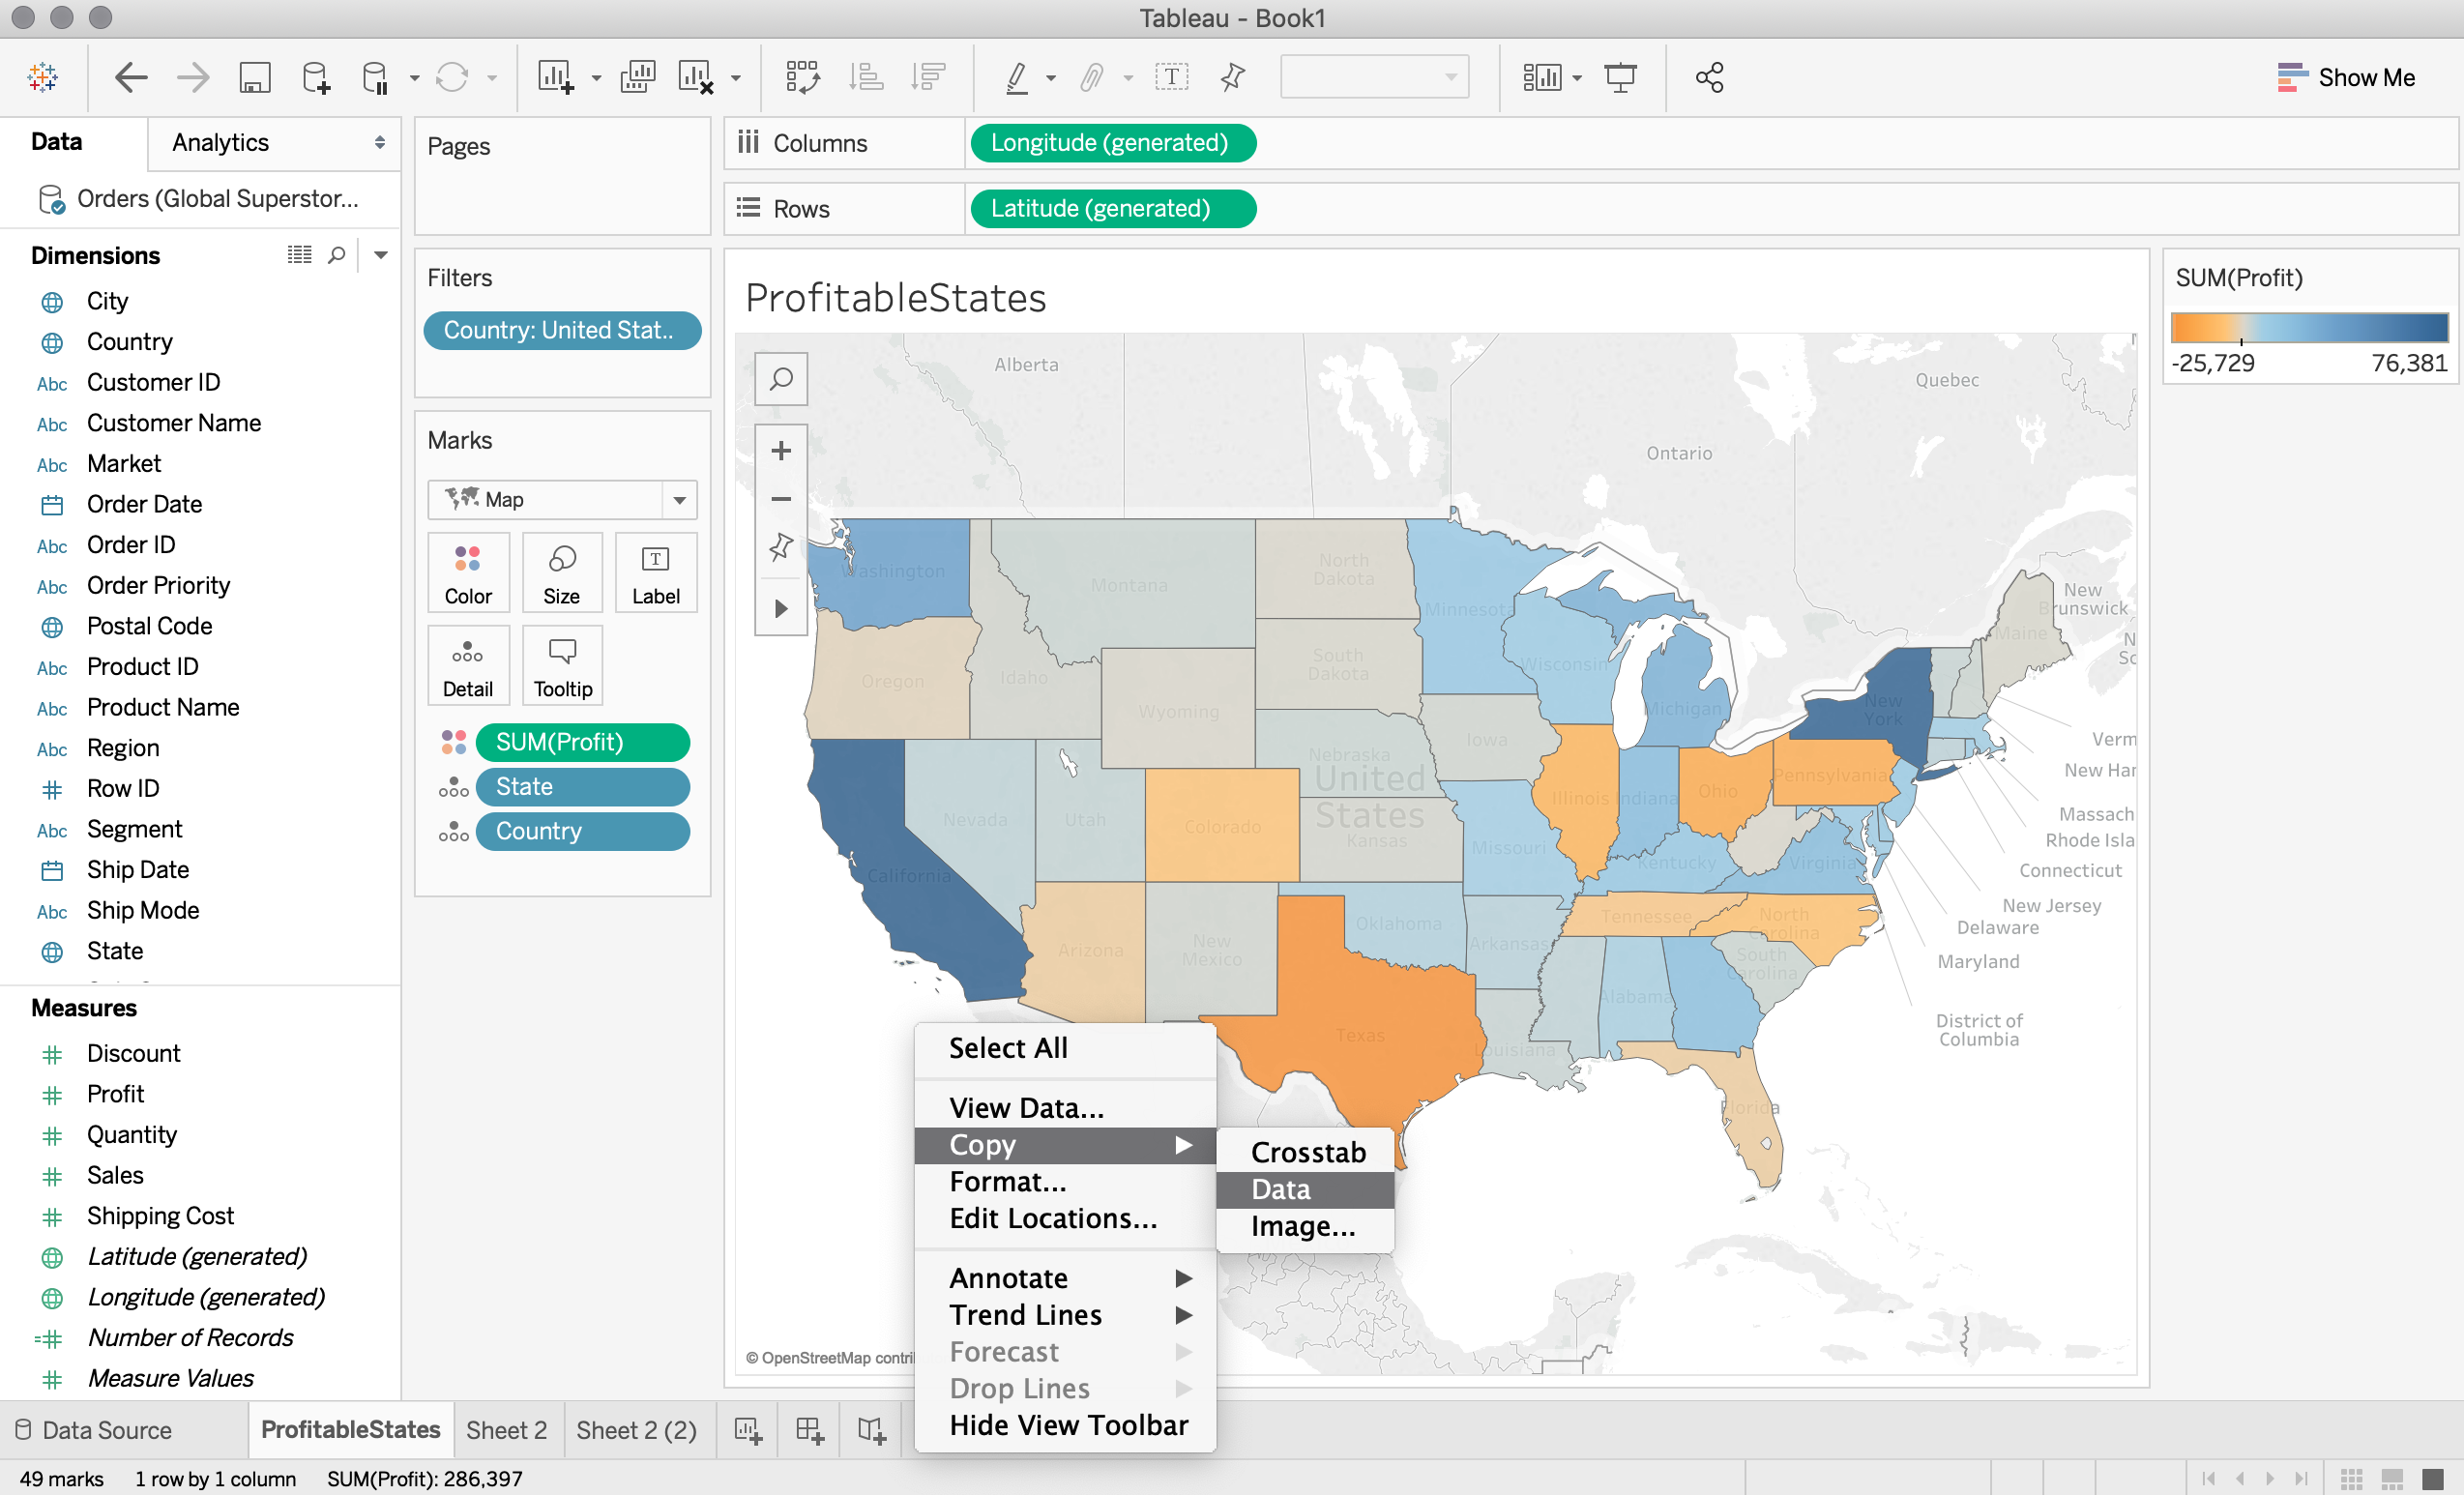
\includegraphics[width=.9\textwidth]{img/copy}
\end{center}
\end{frame}

\begin{frame}
\ft{Paste into Excel}
\begin{center}
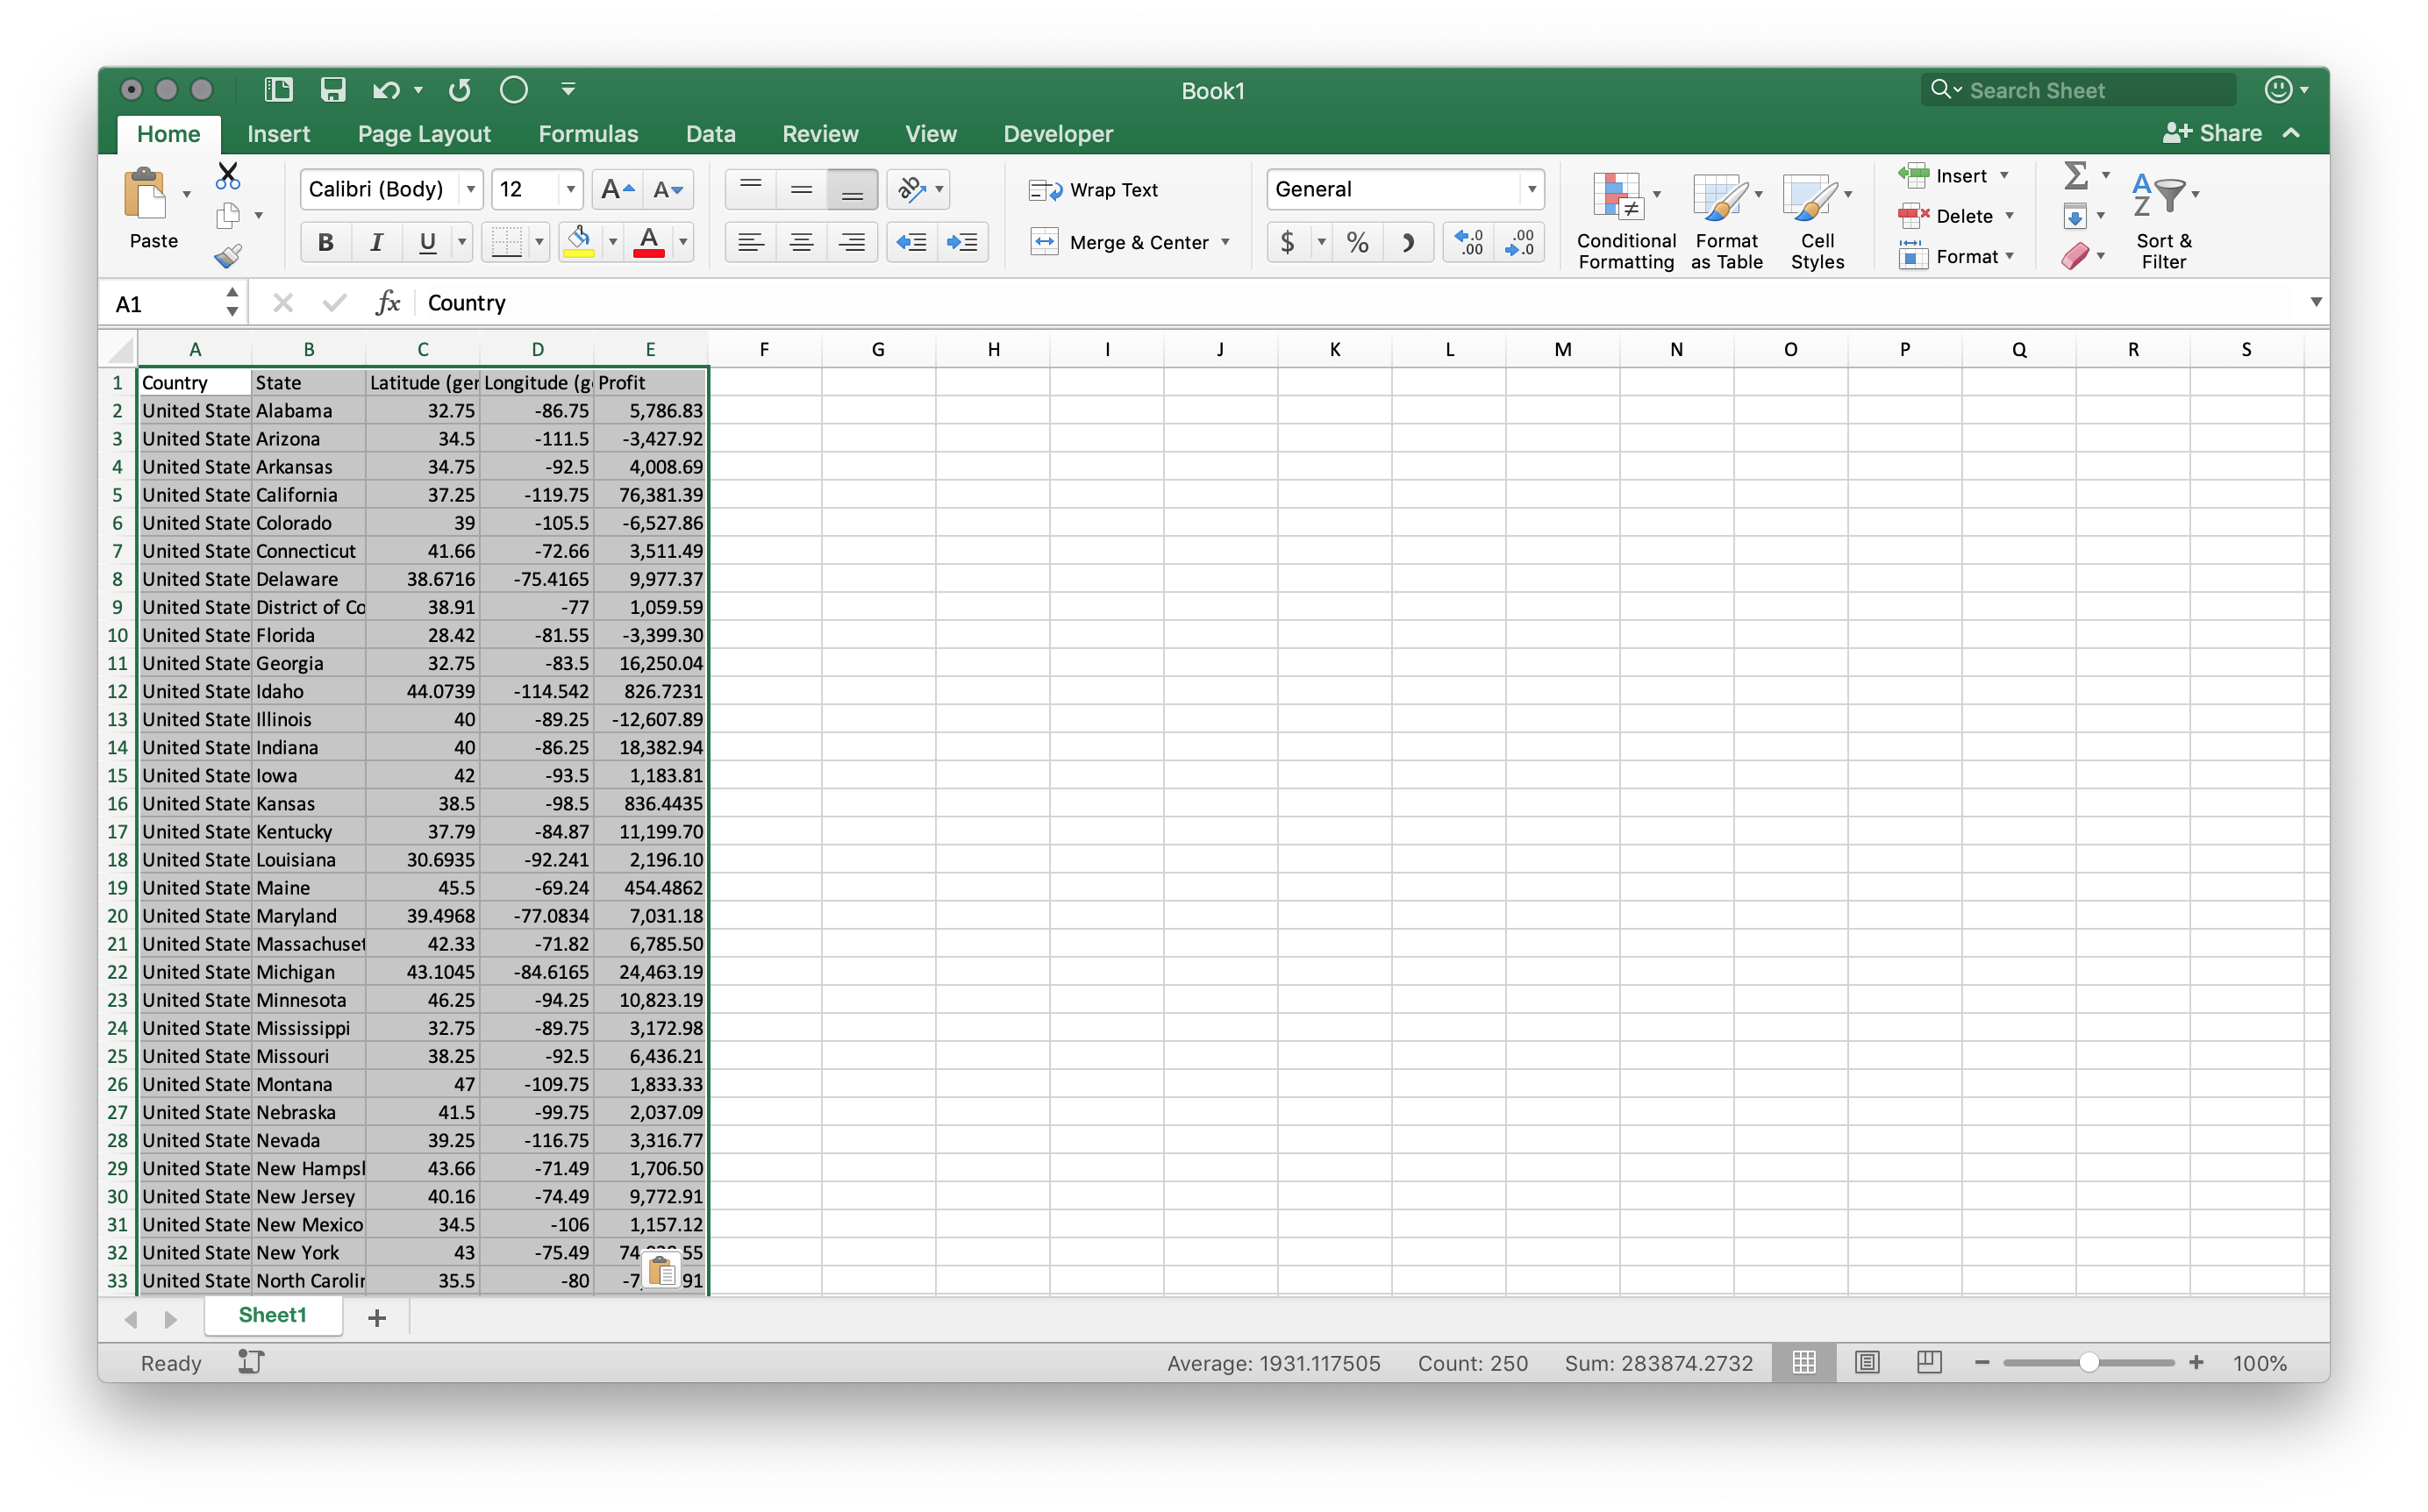
\includegraphics[width=.9\textwidth]{img/paste}
\end{center}
\end{frame}

\begin{frame}
\ft{Duplicate as crosstab}
\begin{center}
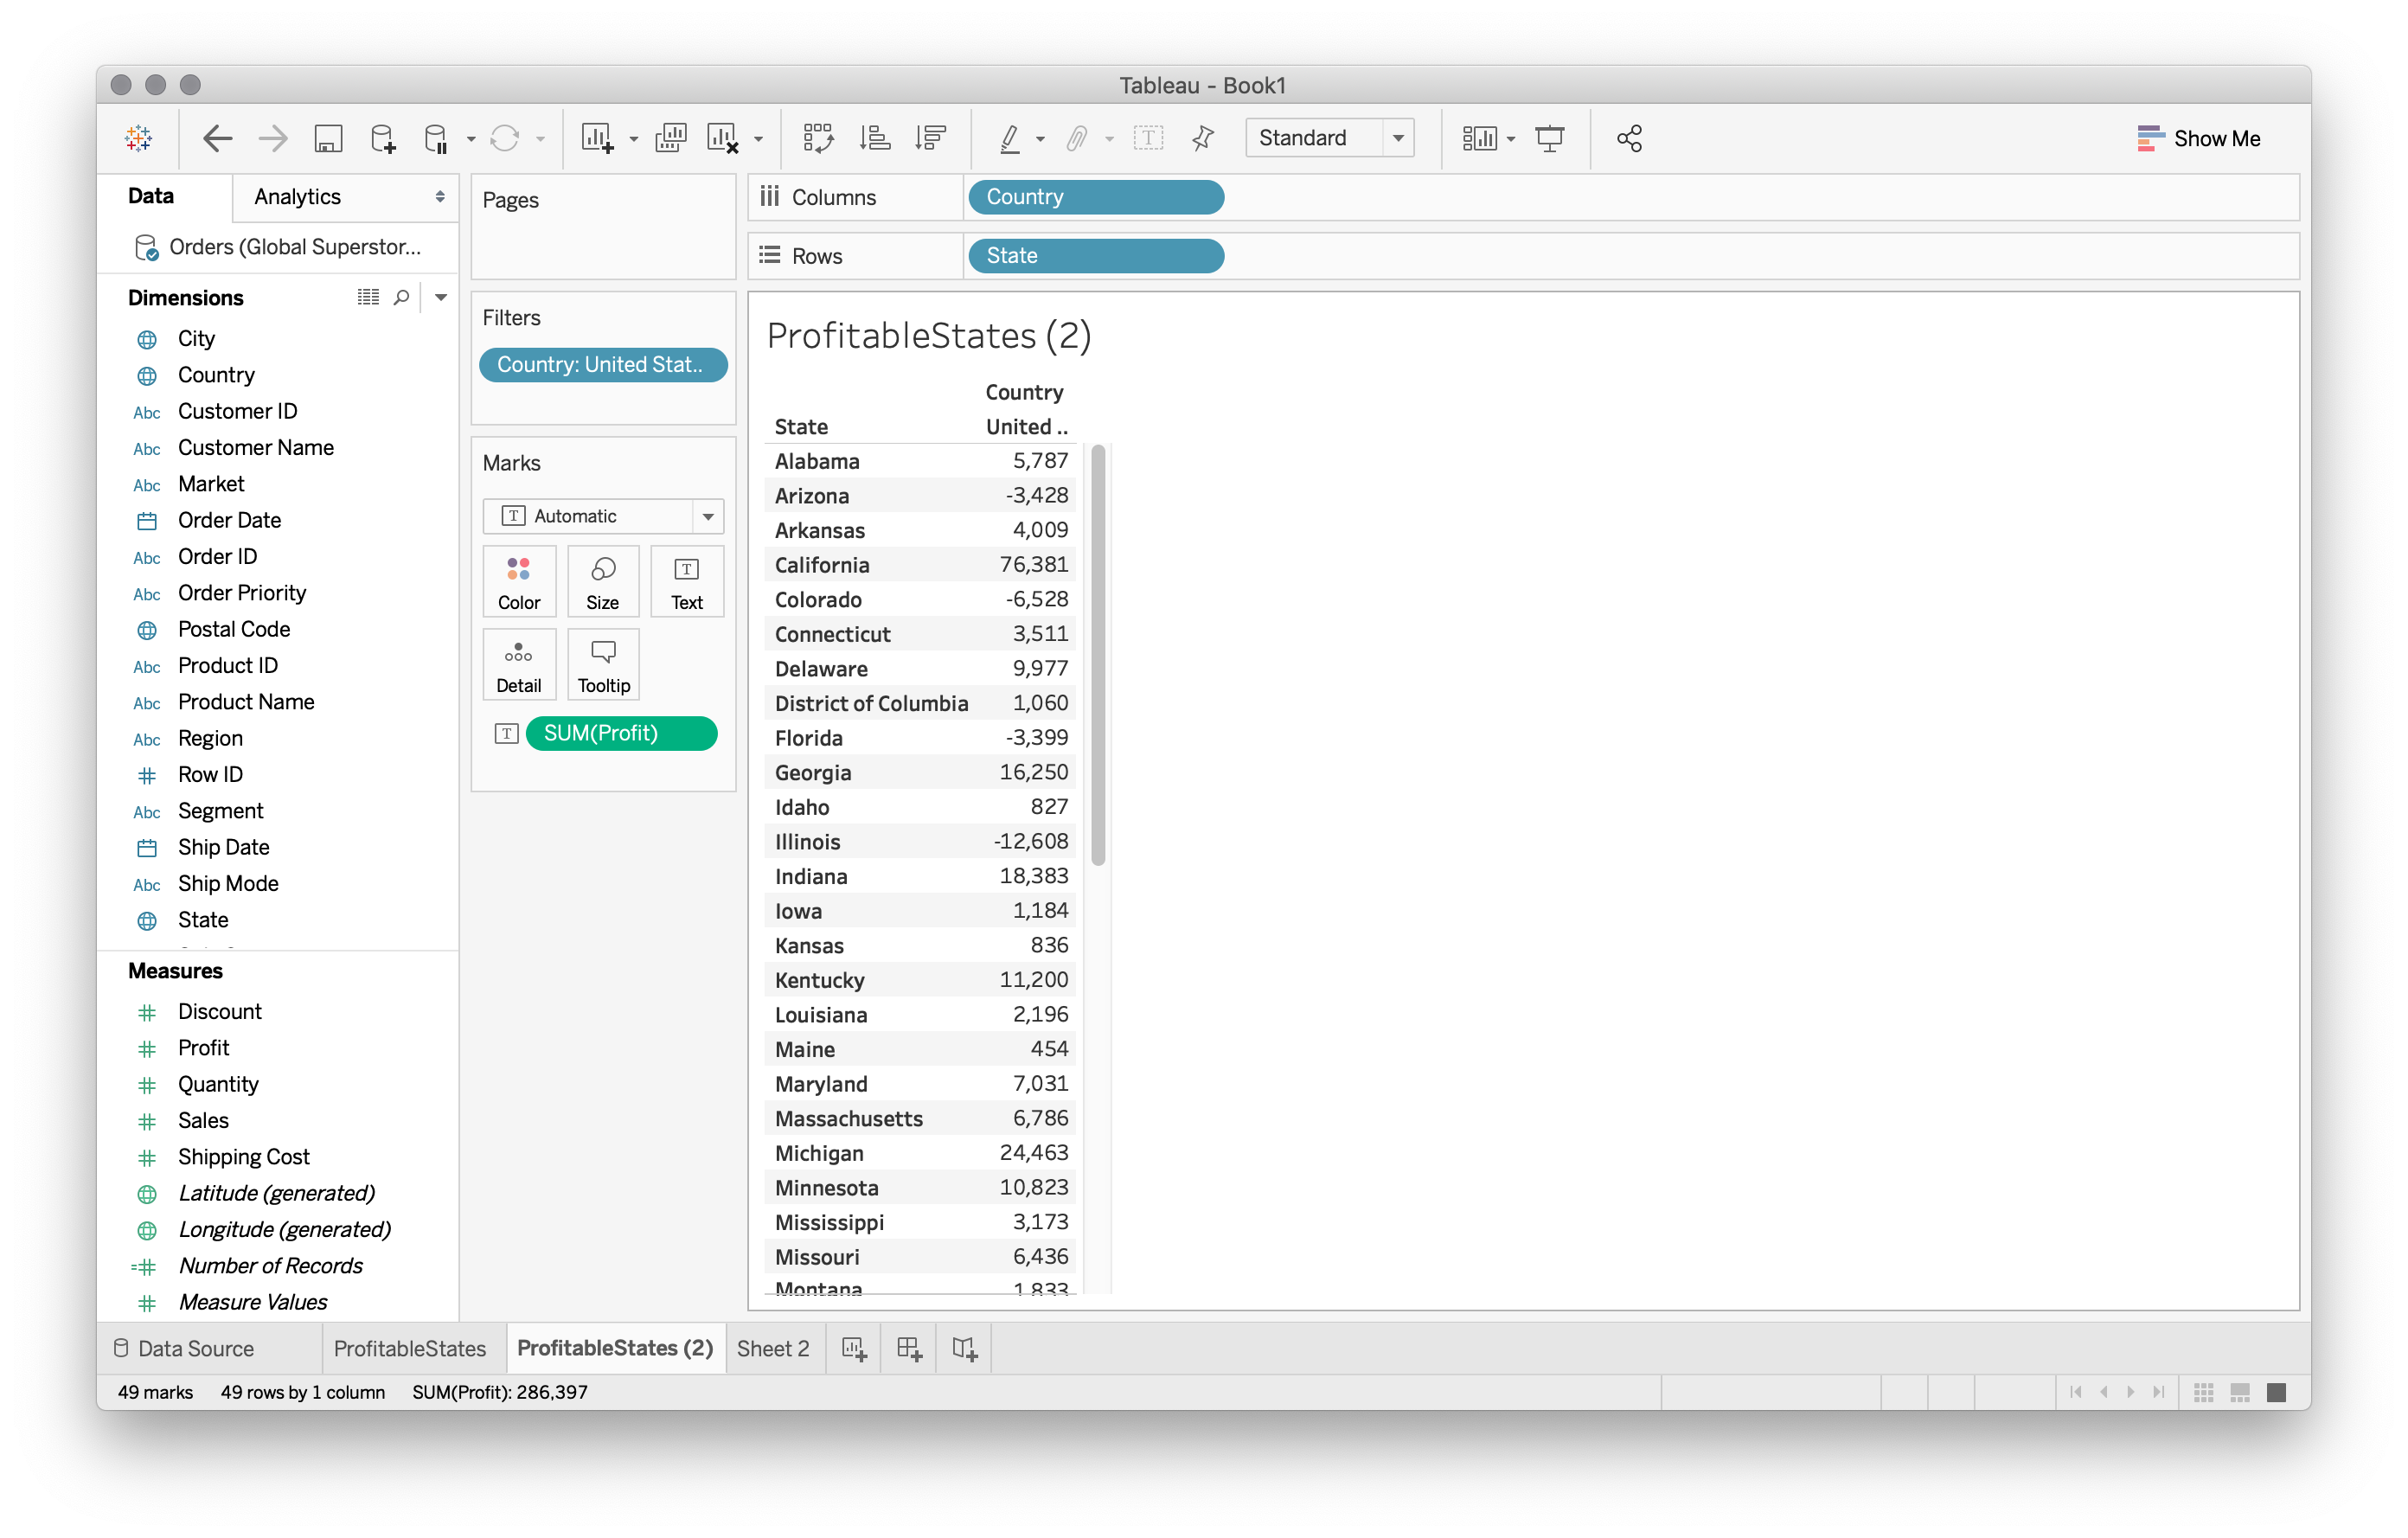
\includegraphics[width=.9\textwidth]{img/crosstab2}
\end{center}
\end{frame}


\begin{frame}
\ft{Interactive plots}
We can also make the plot interactive by right clicking a desired field and selecting  "Show Filter".
%\begin{center}
%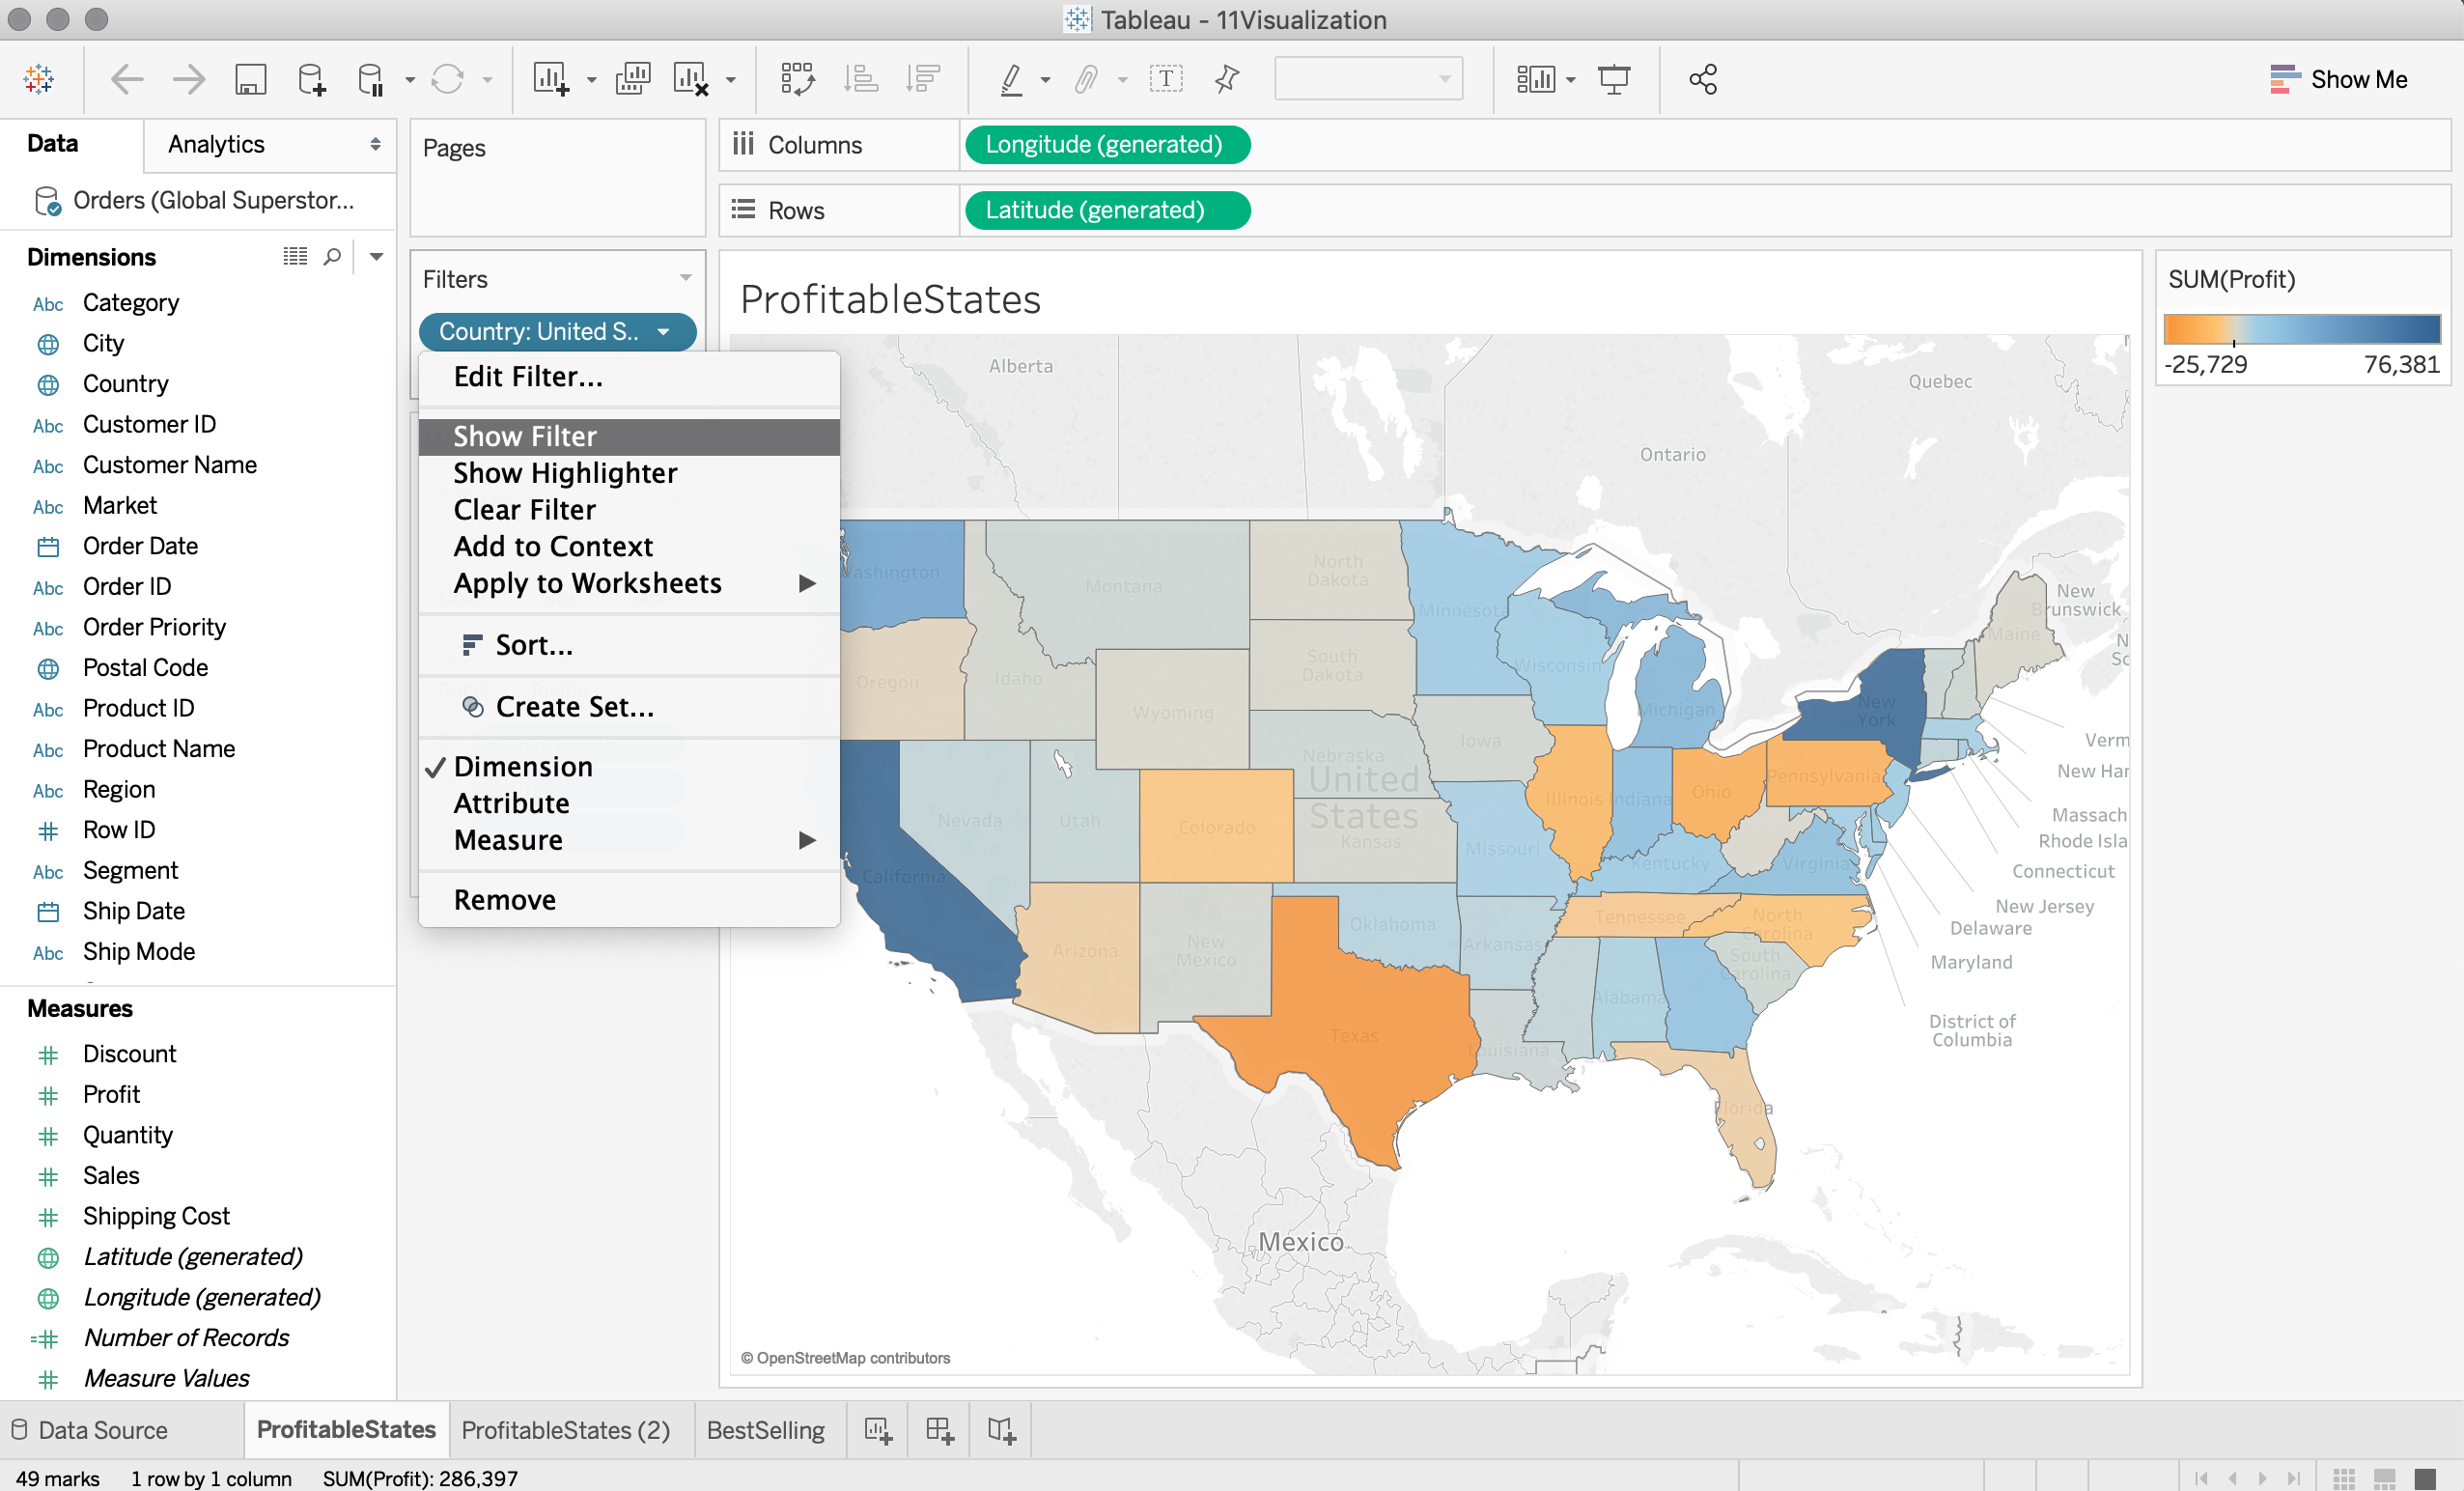
\includegraphics[width=.9\textwidth]{img/showFilter}
%\end{center}
%There are other choices for these lists in the drop down menu.
\vfill
For instance, if we select "Show Filter" for  {\tt Country}, the list of countries will appear in the right hand panel of our graphic.
\vfill 
The user can now select of deselect other countries for our visualization or "viz"
%\begin{center}
%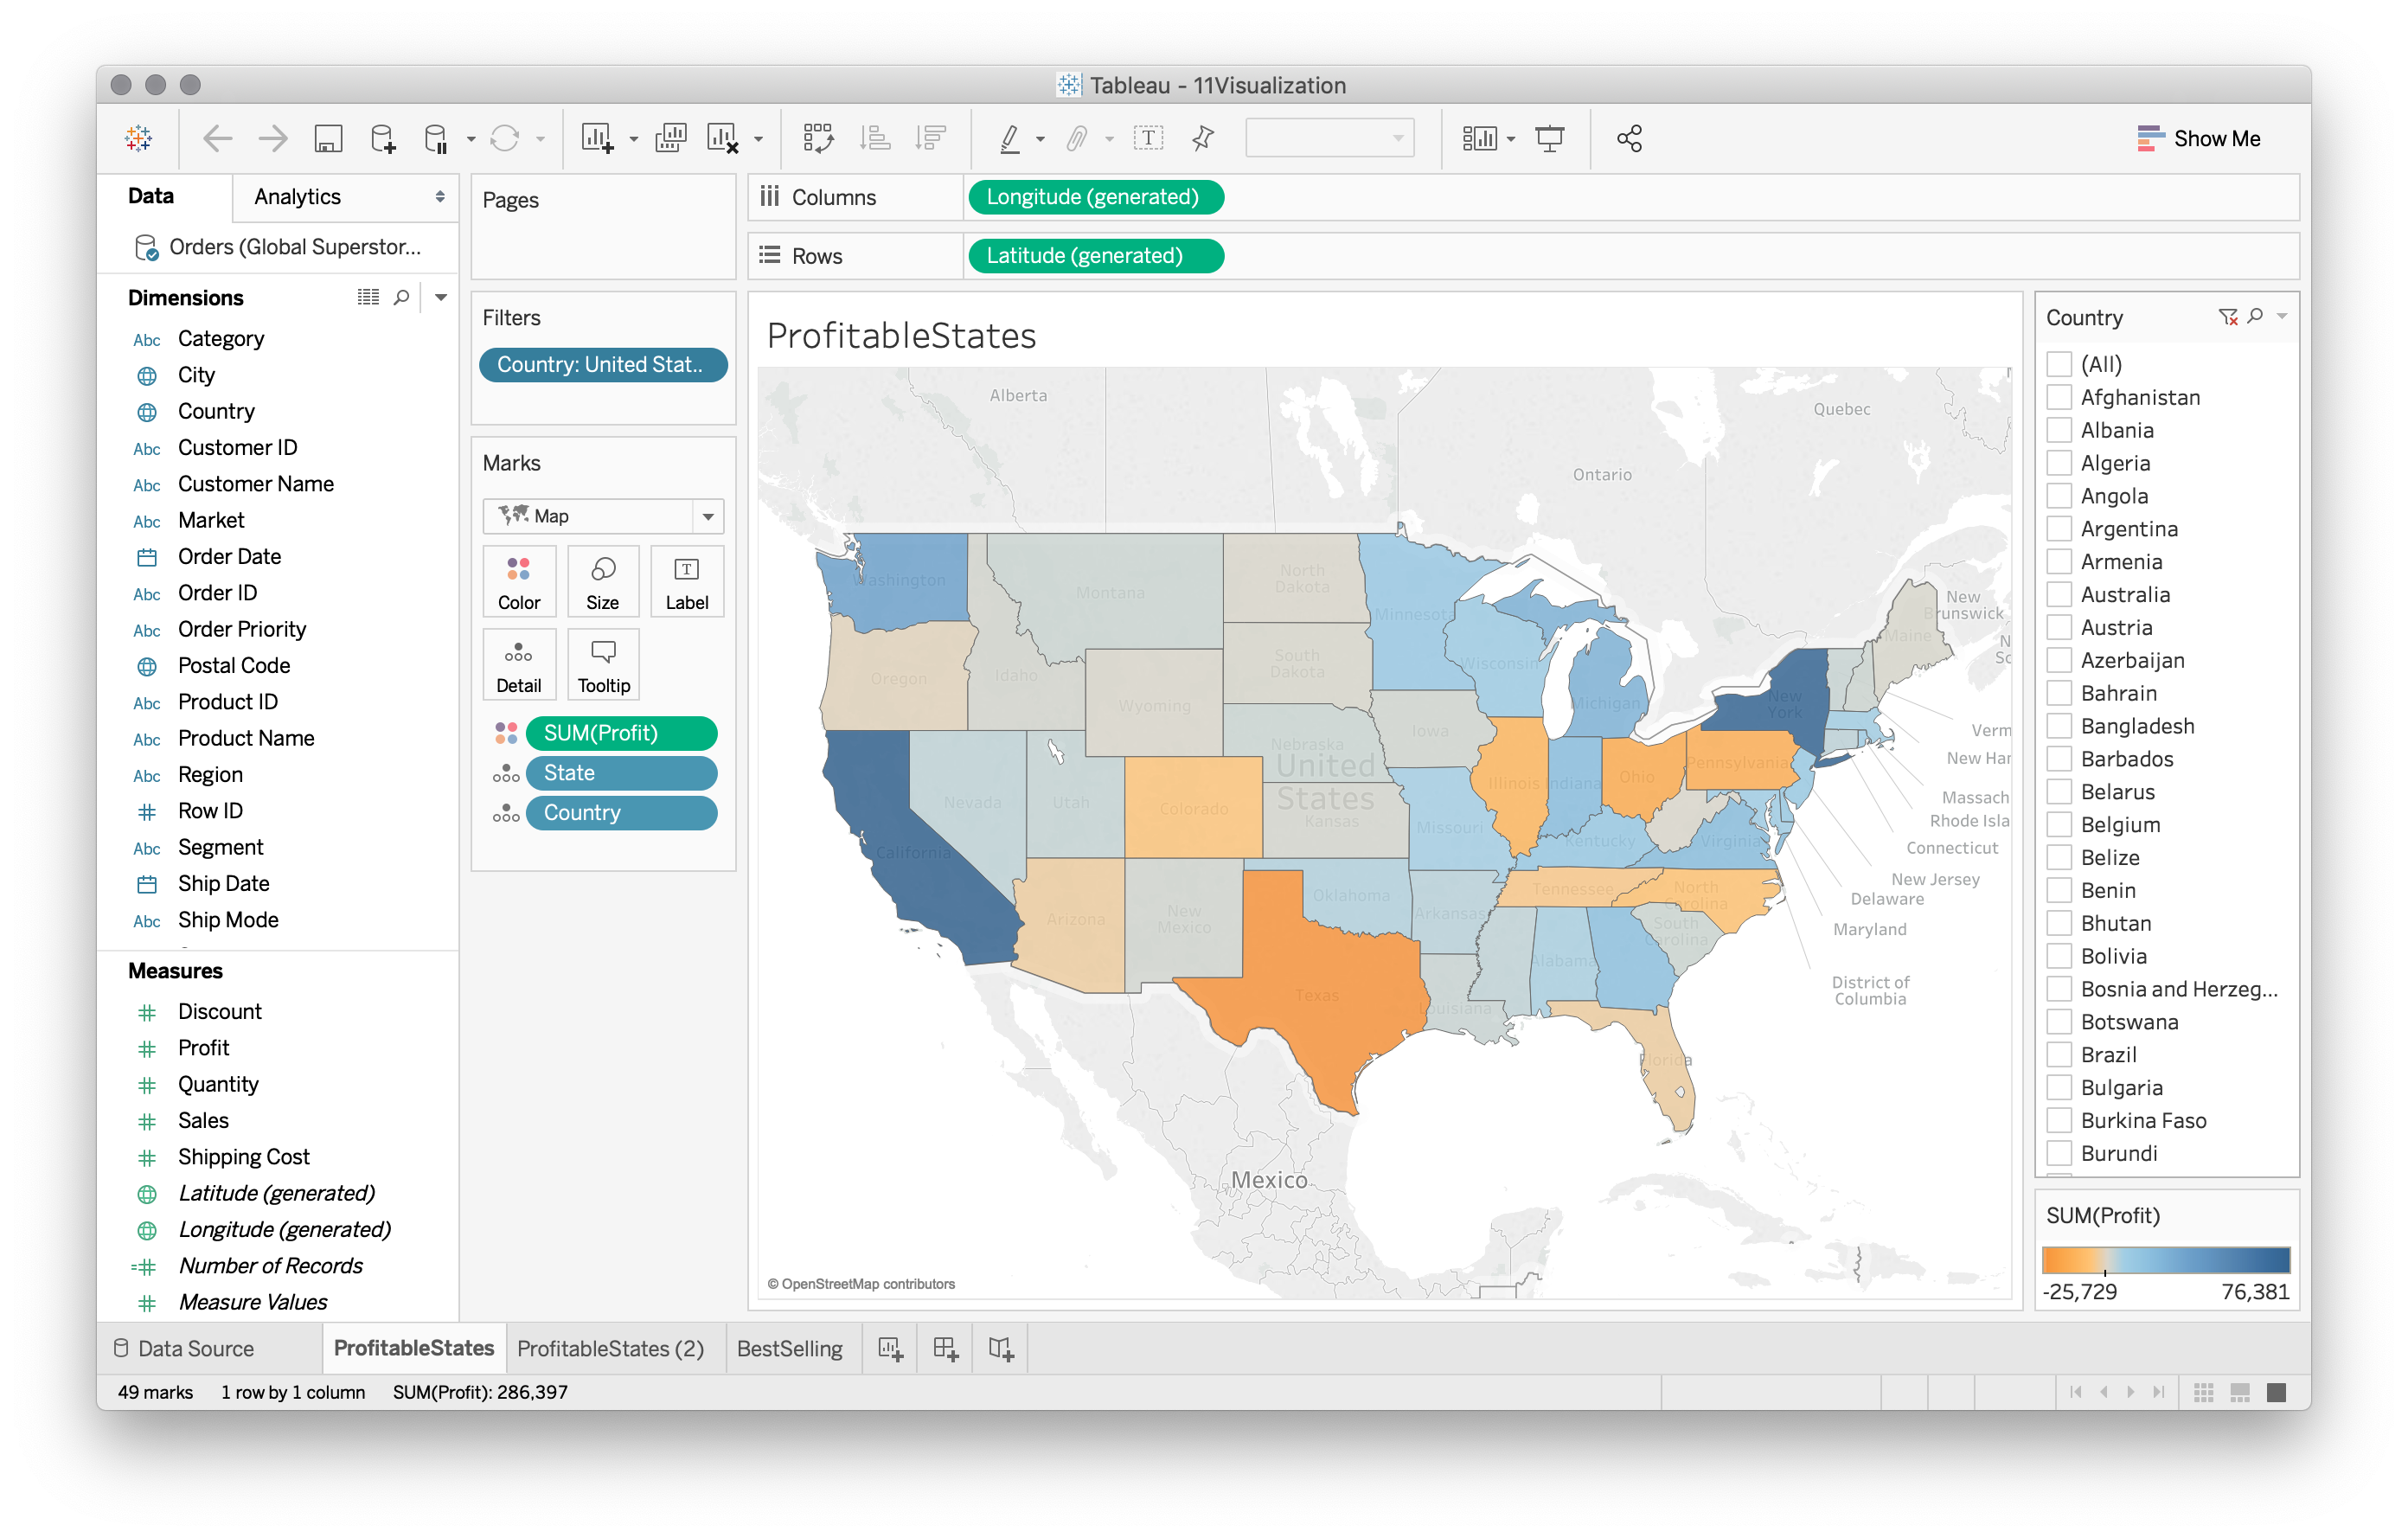
\includegraphics[width=.9\textwidth]{img/interactive}
%\end{center}
\end{frame}


\begin{frame}\ft{Subcategories}
\begin{itemize}
\item \define{Hierarchies} are groupings of data that make it easier to roll-up and drill-down into data.
Examples: 
\begin{itemize}
\item year, quarter, month
\item country, state, city
\end{itemize}
\vfill
\item We can create own hierarchies by dragging dimensions on top of each other. \vfill
%\item Sometimes data will have a natural hierarchical structure.\vfill
\item For example, in the Superstore data, `Sub-category' is a, for lack of better term, sub-category of `Category'.\vfill
\item To have Tableau recognize it as such, we simply drag the sub-category pill over-top of category (in addition, we could do that with product name).  \vfill
\item We might name this new pill `Product'.\vfill
\end{itemize}
\end{frame}

\begin{frame}
\ft{User made dimension}
Notice that the `Product' pill now has a clickable + sign to expand and collapse the levels of the hierarchy. 
\begin{center}
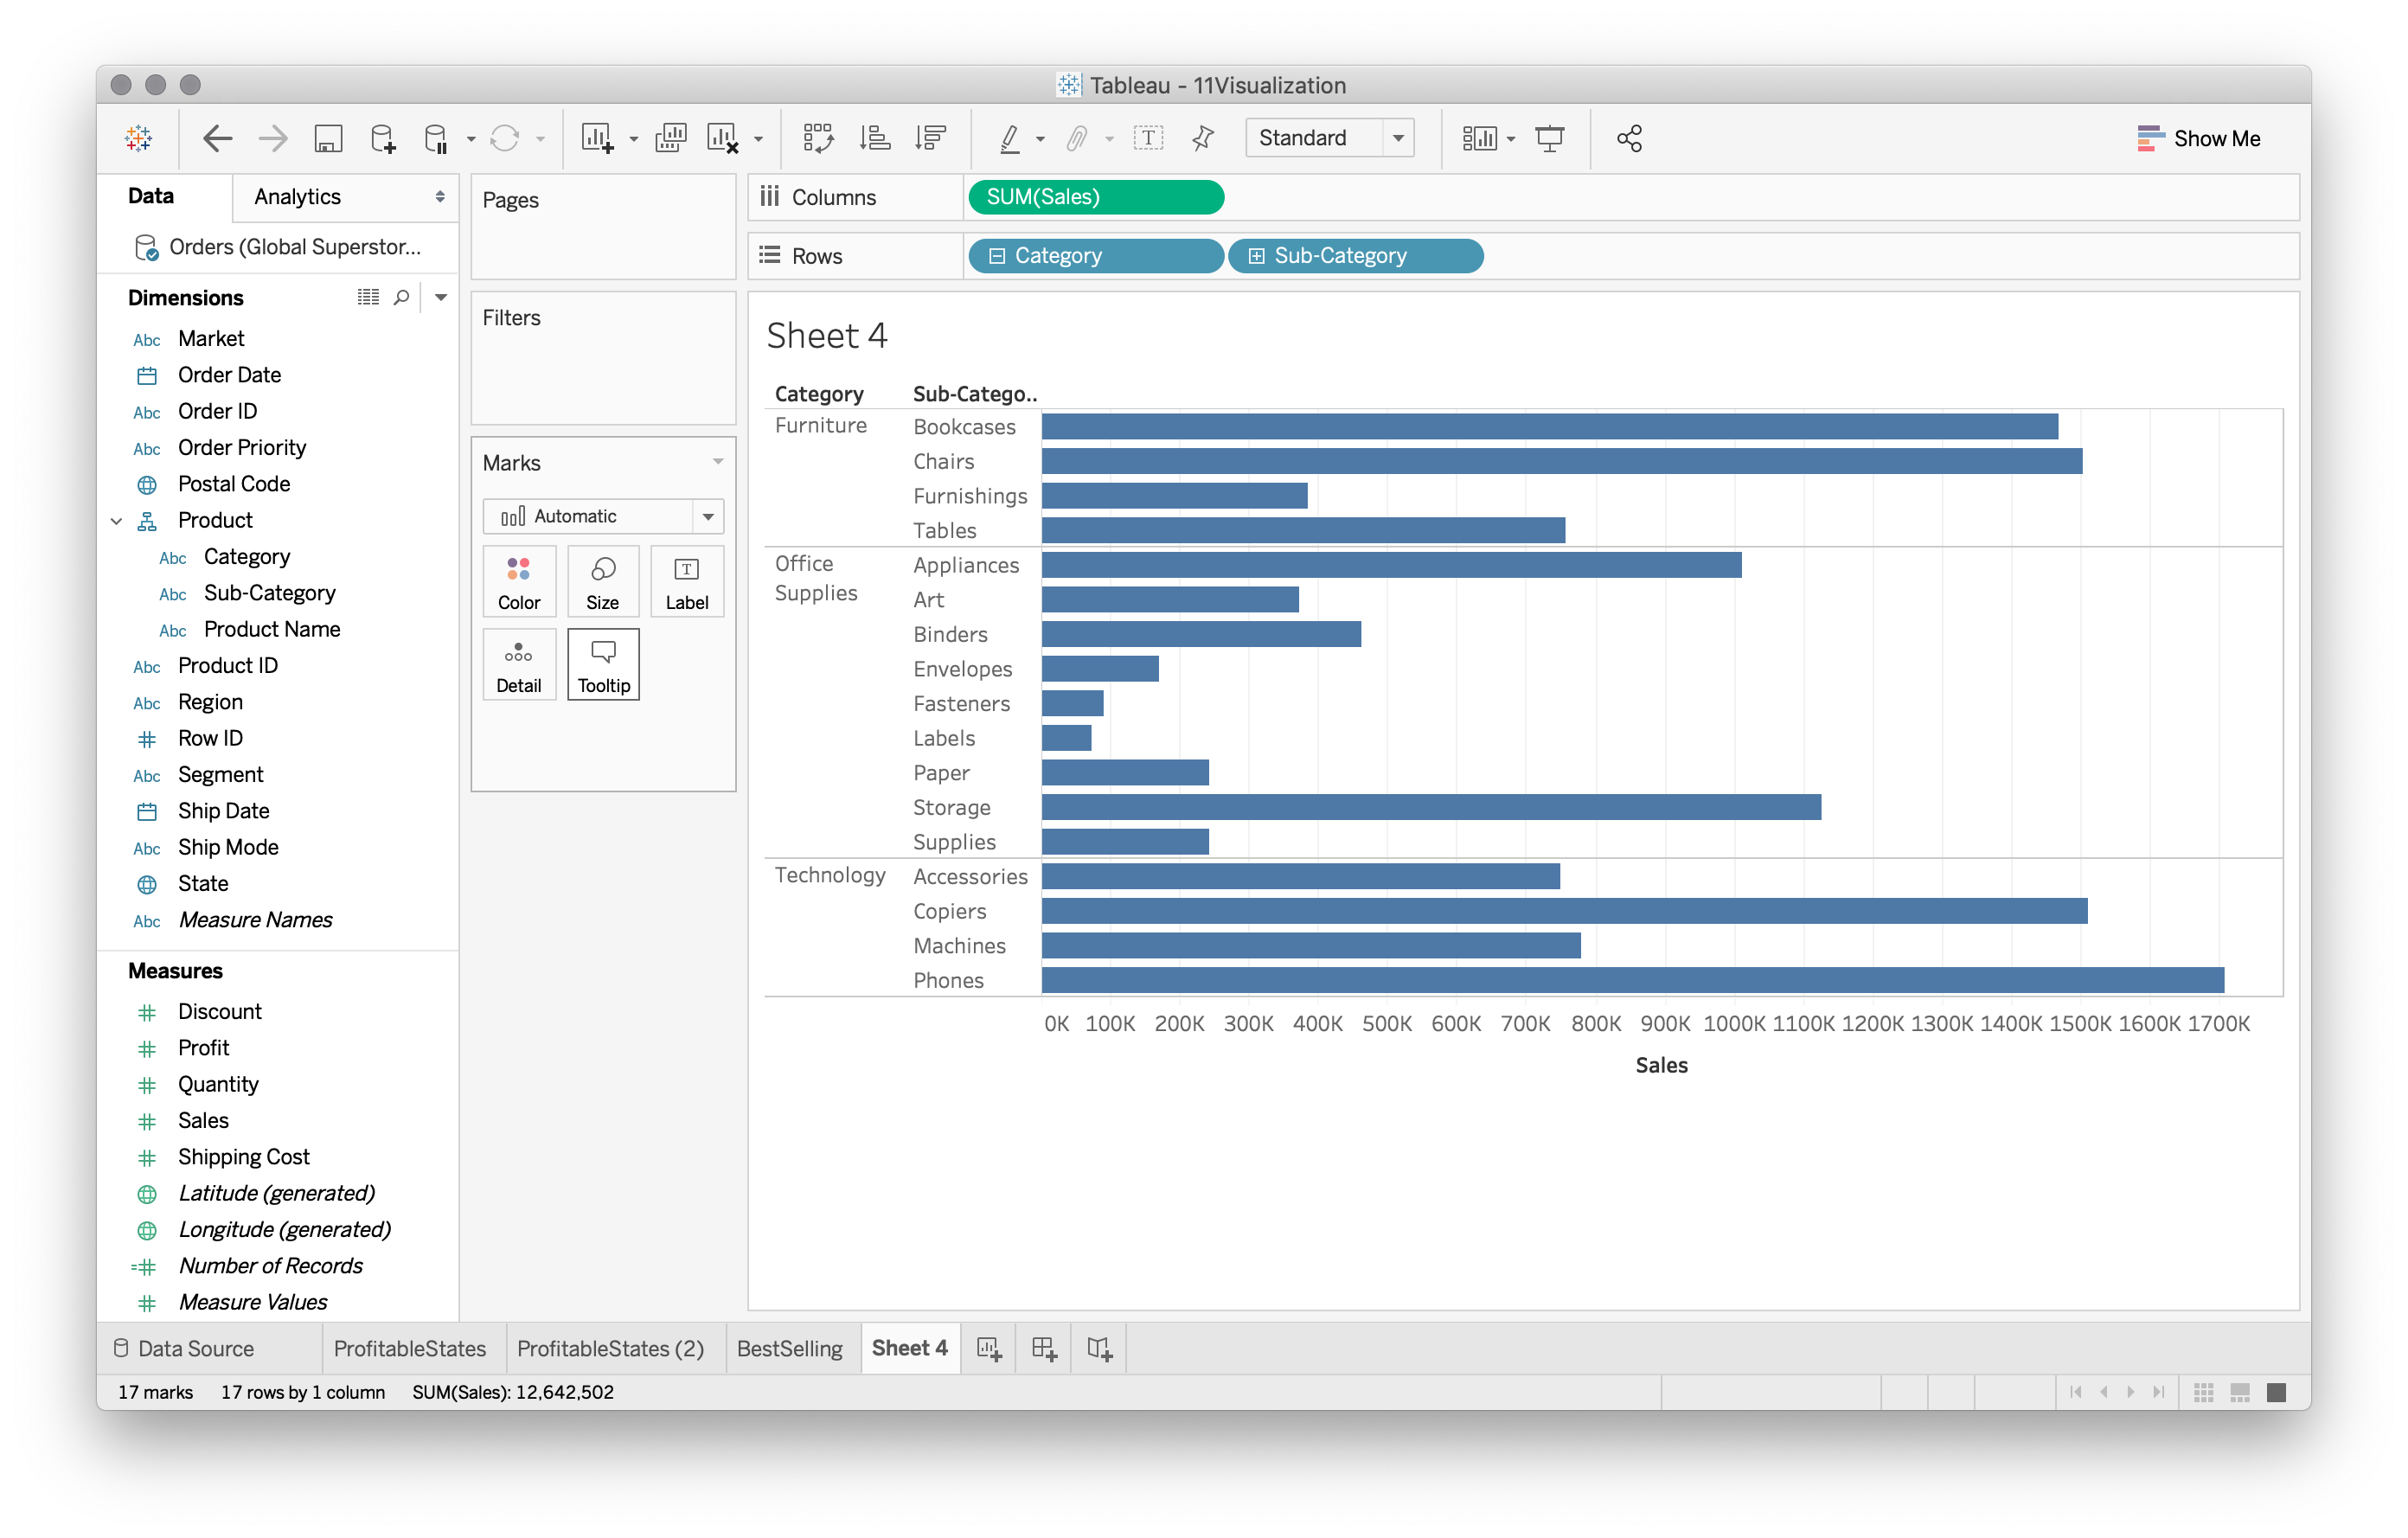
\includegraphics[width=.9\textwidth]{img/product}
\end{center}
\end{frame}


\begin{frame}
\ft{User made dimension}
We can click the sort buttons to arrange bars by descending/ascending order.
\begin{center}
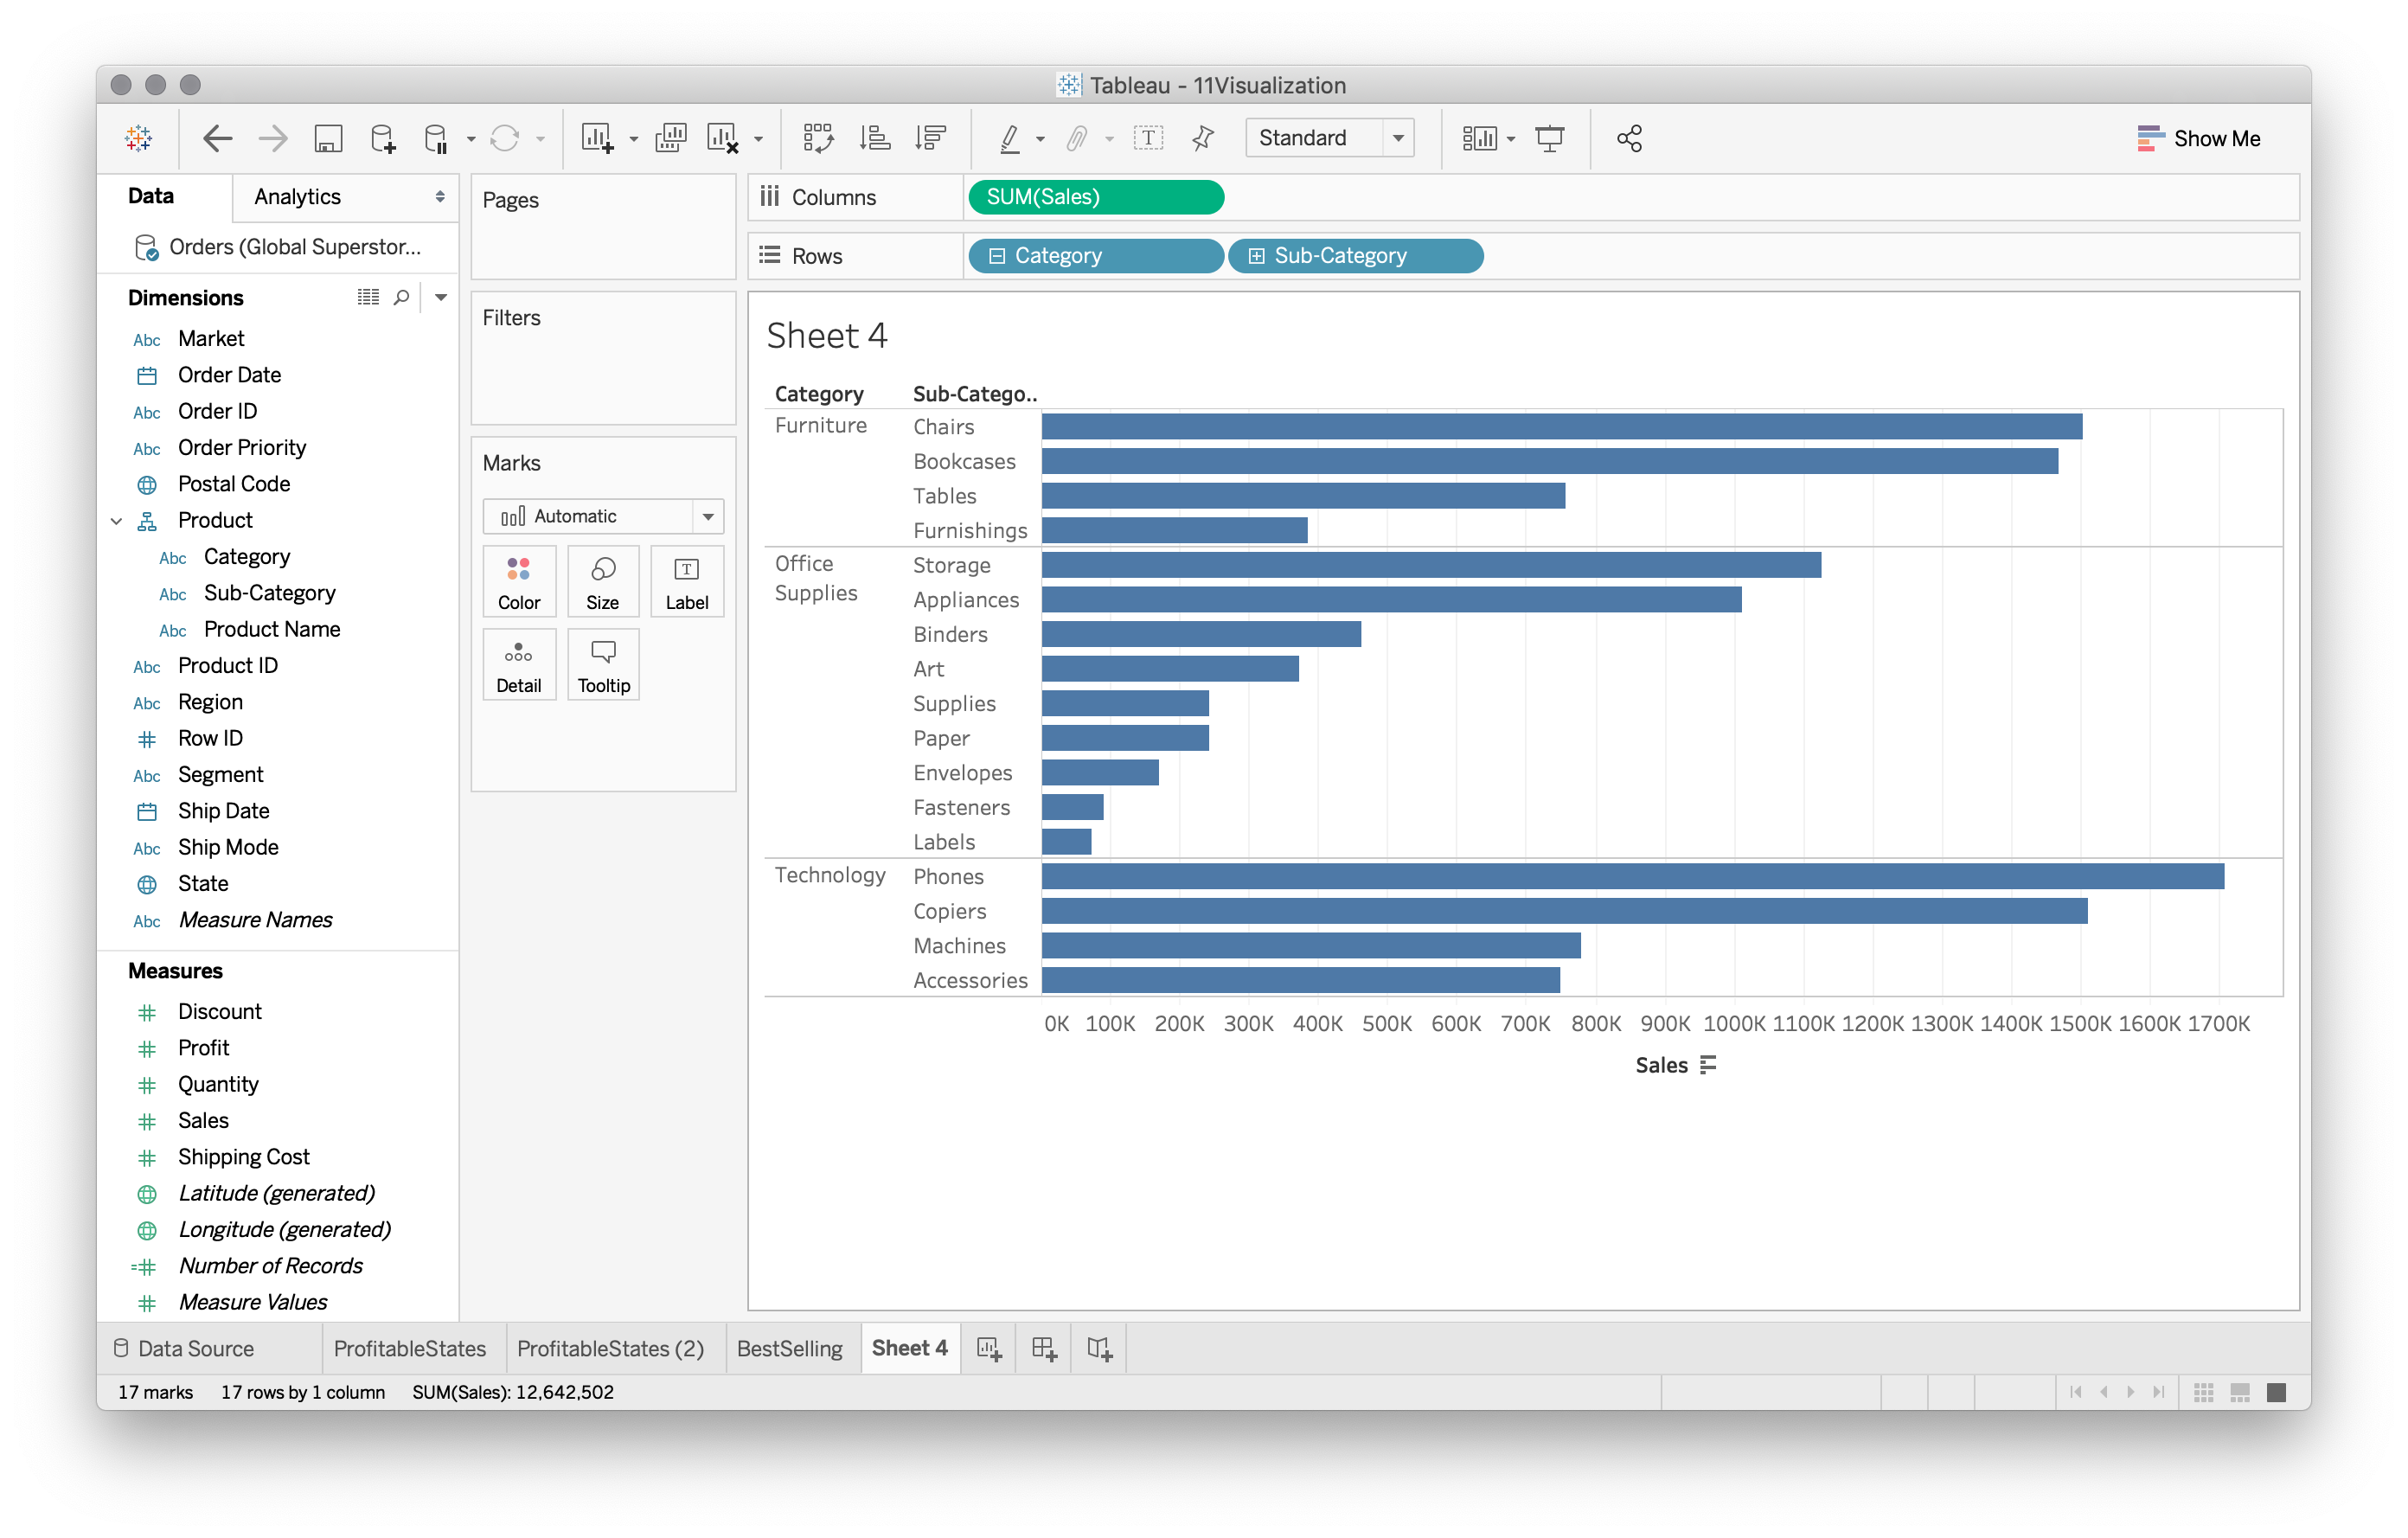
\includegraphics[width=.9\textwidth]{img/sort}
\end{center}
\end{frame}



\begin{frame}\ft{Tableau Files}
\begin{description}
\item [Tableau Workbook (.twb) (default)]  saves workbook but no data
\item [Tableau Packaged Workbook (.twbx)]  contains data and visualization for easier sharing
\item [Tableau Datasource (.tds)]  metadata on a data source
\item [Tableau Bookmark (.twb)]  one worksheet within workbook
\item [Tableau Data Extract (.tde)]  compressed snapshot of data stored in column format
\end{description}

%Note similarities with Excel/spreadsheet terminology.


\end{frame}



\begin{frame}\ft{Joining Tables}
 When connecting tables \define R and \define S, there are four types of joins:
\begin{description}
\item [INNER JOIN] row in result for each row of R that matches a row of S
\item [LEFT OUTER JOIN] row in result for each row of R that matches a row of S OR a row of R that does not match anything in S
\item [RIGHT OUTER JOIN] row in result for each row of R that matches a row of S OR a row of S that does not match anything in R
\item [FULL OUTER JOIN] row in result for each row of R that matches a row of S OR a row of R that does not match anything in S OR a row of S that does not match anything in R
\end{description}
See \href{https://www.codeproject.com/Articles/33052/Visual-Representation-of-SQL-Joins}{here} for a visual representation of joins (for SQL but same concept here).
\end{frame}

\begin{frame}
\ft{Join Example}
\includegraphics[width=1.\textwidth]{img/joins}
\end{frame}

%\begin{frame}
%
%\begin{figure}[htbp]
%\begin{example}
%Given the tables below how many rows are in the result of Boys LEFT OUTER JOIN Girls ON Bid=Gid?
%\tans{2}{8}
%\end{example}
%
%\begin{center}
%\includegraphics[width=.4\textwidth]{img/boys}
%\includegraphics[width=.4\textwidth]{img/girls}
%\caption{Left: Boys Right: Girls}
%\label{join}
%\end{center}
%\end{figure}
%
%\end{frame}
%% i think the answer should be 6 but Ramon says its 8




\begin{frame}\ft{Data Blending}
Data blending allows "joining" data that does not reside in a single source.  There are automatic and manual methods.
\begin{description}
\item [Automatic] field names must match across sources. Will link secondary data source with primary data source.
\item [Manual] methods include ability to specify SQL statement to perform with join.

\end{description}
\end{frame}

\begin{frame}\ft{Try it: Tableau Data Sources - Joins}
Using the MySQL tables in the data301 database, create some joins to connect them so it looks like this:
\includegraphics[width=1.1\textwidth]{img/mySQLjoin.png}


\end{frame}



\begin{frame}\ft{Dynamic Grouping/Renaming}
\begin{itemize}
\item Dynamic grouping (also called ad hoc groups) can be created by using Ctrl+Select (windows) or Cmnd+select (mac) to select elements in visualization and select Group from menu.\vfill
\begin{center}
\includegraphics[width=.45\textwidth]{img/group1}\includegraphics[width=.45\textwidth]{img/group2}
\end{center}


\item It is also possible to rename values/labels and correct value errors.
\begin{itemize}
\item Eg. change California to "CA" by right clicking on the state and selecting {\bf Annotate} > {\bf Mark} and edit the defaults
\end{itemize}


\end{itemize}
\end{frame}


\begin{frame}\ft{Tableau Chart Types}
Chart types:

\begin{itemize}
\item  text tables/crosstabs
\item  maps
\item  heat maps, highlight tables, tree maps
\item  line charts
\item  area fill charts and pie charts
\item  scatter plot, circle view, side-by-side plots (identify outliers)
\item  bullet graph, packed bubble, histogram, Gantt charts
\end{itemize}
\end{frame}

\begin{frame}\ft{Line Chart (discrete time)}
\begin{center}
\includegraphics[width=.9\textwidth]{img/line}
\end{center}
\end{frame}

\begin{frame}\ft{Text Table (Crosstab)}\label{crosstab}
These are very similar to Pivot Tables: after selecting the Dimensions you want, drag the desired Measure directly overtop the table.  N.B. you can change the aggregate function (SUM is the default in most cases)
\begin{center}
\includegraphics[width=.9\textwidth]{img/crosstab}
\end{center}
\end{frame}


\begin{frame}\ft{Maps}
\begin{center}
\includegraphics[width=.9\textwidth]{img/maps}
\end{center}
\end{frame}


\begin{frame}\ft{Heat Map}
%Select the appropriate pills, click `Heat Map' in {\bf Show Me} and drag Sales to `Color' in the  {\bf Marks} panel.
Turn the cross tab viz from slide \ref{crosstab} to a heat map by going to the {\bf Show Me} tab and selecting the option in the top right corner.  Think of this as a complex conditional formatting of Excel cells.
\begin{center}
\includegraphics[width=.9\textwidth]{img/heatmap2}
\end{center}
\end{frame}


\begin{frame}\ft{Tree Map}
Tree maps  are a way of displaying hierarchical data using nested figures, usually rectangles.
To change the colours used, click `Color' in the  {\bf Marks} panel and go to Edit Colors.
\begin{center}
\includegraphics[width=.9\textwidth]{img/treemap}
\end{center}
\end{frame}


\begin{frame}\ft{Bar Charts}

\begin{center}
\includegraphics[width=.9\textwidth]{img/bar}
\end{center}
\end{frame}


\begin{frame}\ft{Pie Charts}
\begin{center}
\includegraphics[width=.9\textwidth]{img/piecharts}
\end{center}
\end{frame}



\begin{frame}\ft{Scatter Plots}
You can change the points that appear in your scatterplot by dragging pills into the {\bf Details} button in the marks field.
\begin{center}
\includegraphics[width=.9\textwidth]{img/scatter}
\end{center}
\end{frame}








\begin{frame}\ft{Trend Lines and Reference Lines}
\begin{itemize}
\item Trend lines show patterns in data.\vfill

\item Trend lines can be easily created by:
\begin{itemize}
\item  navigating the {\bf Analytics} pane $\to$ {\bf Model} $\to$ Trend Line (double click or drag).
\item or by right clicking on appropriate visualizations.\vfill
\end{itemize}
\item These trend lines do not have to be linear.\vfill
\item To remove the trend line, simple drag it off the viz (or press undo).
\item If you hover over the trend line on your Viz, you can see some useful information (eg. p-value, R-squared) in the so-called ``tooltip".
\end{itemize}
\end{frame}


\begin{frame}
\ft{Adding Trend Lines}
\begin{center}
\includegraphics[width=.9\textwidth]{img/trendlineSP}
\end{center}
\end{frame}


\begin{frame}
\ft{Adding Trend Lines}
\begin{center}
\includegraphics[width=.9\textwidth]{img/dragTrend}
\end{center}
\end{frame}

\begin{frame}
\ft{Adding Trend Lines}
\begin{center}
\includegraphics[width=.9\textwidth]{img/rightClickTrend}
\end{center}
\end{frame}



\begin{frame}\ft{Trend Lines and Reference Lines}
\begin{itemize}
\item We can get `side-by-side' or colour-coded trendlines for multiple fields by dragging an additional dimension into the view.
\item For example:
\begin{itemize}
\item Navigate back to the Data pane
\item Drag {\bf Location} onto the $y$-axis of the Viz (or the Row shelf) see \hyperlink{trippleTrend}{Figure 1}
\item Alternatively we could drag {\bf Location} onto `Color' on the {\bf Marks} pane: see \hyperlink{trippleTrend2}{Figure 2}
\end{itemize}
\end{itemize}
\end{frame}

\begin{frame}
\ft{Adding Trend Lines}
\begin{figure}[htbp]
\begin{center}
\includegraphics[width=.9\textwidth]{img/trippleTrend}
\caption{default}
\label{trippleTrend}
\end{center}
\end{figure}

\end{frame}


\begin{frame}
\ft{Adding Trend Lines}
\begin{figure}[htbp]
\includegraphics[width=.9\textwidth]{img/trippleTrend2}
\caption{default}
\label{trippleTrend2}
\end{figure}
\end{frame}


\begin{frame}
\ft{Reference Lines}
\begin{itemize}
\item Reference lines allow comparison with a reference (detect trends and outliers). To add a reference line:
\begin{itemize}
\item  go to the {\bf Analytics} tab $\to$ {\bf Custom} pane ``Reference Line"
\item or right click on the $y$ (or $x$) axis on the Viz and select {\bf Add Reference Line}.
\end{itemize}
\item To show the confidence bands, right click your trend line, {\bf Trend Lines} $\to$ {\bf Edit Trend Lines...} and select "Show Confidence Bands"
\begin{center}
\includegraphics[width=.45\textwidth]{img/CB}
\end{center}
\end{itemize}


\end{frame}

\begin{frame}
\ft{Adding Trend Lines and Reference Lines}
\begin{center}
\includegraphics[width=.9\textwidth]{img/trendref}
\end{center}
\end{frame}






%\begin{frame}
%\ft{Adding Quantiles}
%\begin{center}
%\includegraphics[width=.9\textwidth]{img/quantiles}
%\end{center}
%\end{frame}

\begin{frame}
\ft{Sorting}
\begin{center}
\includegraphics[width=.9\textwidth]{img/sorting}
\end{center}
\end{frame}




%\begin{frame}\ft{Hierarchies}
%\define{Hierarchies} are groupings of data that make it easier to roll-up and drill-down into data.
%Examples: 
%\begin{itemize}
%\item category and subcategory
%\item year, quarter, month
%\item country, state, city
%\end{itemize}
%Can create own hierarchies by dragging dimensions on top of each other.
%\end{frame}

%\begin{frame}\ft{Filters}
%There are multiple ways to define filters:
%\begin{itemize}
%\item  Drag dimension into filter shelf
%\item   Quick filters allow people using report to change filters dynamically. (click on item in filter shelf and select Show Filter option)
%
%\end{itemize}
%\end{frame}



%\begin{frame}
%\ft{Grouping}
%\define{Grouping} allows summarizing data without using a hierarchy.
%\begin{itemize}
%\item Multi-select elements then in pop-up menu select Group
%\end{itemize}
%\begin{center}
%\includegraphics[width=.9\textwidth]{img/group}
%\end{center}
%\end{frame}


%\begin{frame}
%\ft{Calculations}
%\define{Calculated fields} are performed on data source when possible.
%\define{Table calculations} are performed locally in Tableau.
%\begin{center}
%\includegraphics[width=.6\textwidth]{img/calc}
%\end{center}
%\end{frame}


\begin{frame}
\ft{Calculations}
\begin{itemize}
\item Functions in tableau allow us to manipulate our data.
\item We can save those calculations in a \define{calculated field}.
\item To create a calculated field, simply right click in the data pane and select {\bf Create} $\to$ {\bf Calculated Field}
\end{itemize}
\begin{center}
\includegraphics[width=.6\textwidth]{img/calc}
\end{center}
\end{frame}


\begin{frame}
\ft{Calculations}
\begin{itemize}
\item Available functions are displayed on the right hand panel, and our formulas (similar to what you would write in an Excel cell) is written on the left.
\vfill
\item You may search for functions within the right-hand panel.
\vfill
\item Functions work very much the same as in Excel, only now instead of referencing numbers be cell we call on them by name using {\tt [PillName]}. % where {\tt PillName}.
\vfill
\item Notice that the name of our new calculated field will be prefaced by an equal sign \includegraphics[height=1em]{img/equalsign}
\vfill
\item Now, this calculated field may be treated as any other pill.
\vfill
\end{itemize}
\end{frame}



\begin{frame}
\ft{Creating a Calculated Field}
An example calling a function on a String
\begin{center}
\includegraphics[width=.99\textwidth]{img/field}
\end{center}
\end{frame}

\begin{frame}
\ft{Creating a Calculated Field}
An example calling a function on a Number
\begin{center}
\includegraphics[width=.99\textwidth]{img/formula}
\end{center}
\end{frame}

%
%\begin{frame}\ft{Parameters}
%\begin{itemize}
%\item  Calculations may have \define{parameters}. \vfill
%\item Think of these as variables in an equation that may interactively change.\vfill
%\item Parameters may be exposed in the visualization so the user can control them.\vfill
%\item Parameters are only useful when the are used in something else (eg. calculated field, reference line) that depends on its value.
%\begin{itemize}
%\item For example, we might create a parameter to control how the data are colour coded in a scatterplot (see next slides).
%\end{itemize}
%\end{itemize}
%\end{frame}
%
%
%\begin{frame}
%\ft{Parameters}
%Parameter set to 50
%\begin{center}
%\includegraphics[width=.99\textwidth]{img/p50}
%\end{center}
%\end{frame}
%
%\begin{frame}
%\ft{Parameters}
%Parameter set to 500
%\begin{center}
%\includegraphics[width=.99\textwidth]{img/p500}
%\end{center}
%\end{frame}

\begin{frame}
\ft{Forecasting}
\begin{itemize}
\item Forecasts use statistical models to generate predictions for future data based on historical information.\vfill
\item To build a forecast in Tableau, we need a \textit{Date} Dimension pill and a Measure (i.e some green pill).\vfill
\item Once the pills are dragged to the appropriate shelf, navigate to the Analytics tab, and select the Forecast option.\vfill
\item By default, this will create a forecast prediction curve, alongside prediction bands. 
\end{itemize}


\end{frame}

\begin{frame}
\ft{Forecasting}
\begin{center}
\includegraphics[width=.99\textwidth]{img/forecast1}
\end{center}
\end{frame}

\begin{frame}
\ft{Forecasting}
\begin{center}
\includegraphics[width=.99\textwidth]{img/forecast2}
\end{center}
\end{frame}



\begin{frame}
\ft{Forecasting}
Alternatively, we can right click on an appropriate Viz and  select {\bf Forecast} $\to$ {\bf Show Forecast}
\begin{center}
\includegraphics[width=.99\textwidth]{img/forcast}
\end{center}
\end{frame}

\begin{frame}\ft{Tableau Question}
\begin{example}
How many of the following statements are TRUE?
\begin{enumerate}
\item There can only be one pill on the row shelf.
\item A trend line can only be linear.
\item A user can group multiple items into a group in the visualization.
%\item Calculated fields are calculated on the data source if possible.
%\item Filters may be exposed to the user of the visualization just like parameters.
\end{enumerate}
\begin{multicols}{5}
\begin{enumerate}[A)]
\item 0 
\item 1
\item 2
\item 3
\end{enumerate}
\end{multicols}
\end{example}
\end{frame}



\begin{frame}\ft{Tableau Question}
\begin{block}{Answer}
How many of the following statements are TRUE?
\begin{enumerate}
\item There can only be one pill on the row shelf. \pxmark
\item A trend line can only be linear.\pxmark
\item A user can group multiple items into a group in the visualization. \pcmark
%\item Calculated fields are calculated on the data source if possible.\pcmark
%\item Filters may be exposed to the user of the visualization just like parameters.\pcmark
\end{enumerate}
\begin{multicols}{5}
\begin{enumerate}[A)]
\item 0 
\item {\bf 1}
\item 2
\item 3
\end{enumerate}
\end{multicols}

\end{block}
\end{frame}



\begin{frame}\ft{Try it: Tableau Charts}
Using the Superstore data set, create a visualization for each of these chart types:

\begin{itemize}
\item line chart (with forecast and trend line)
\item bar chart (with filters and sorting)
\item pie chart (with a parameter)
\item heat map (with grouping)
\item scatter plot (with a calculated field)
\item histogram
\item circle view
\end{itemize}
\end{frame}

\begin{frame}\ft{Dashboards}

\begin{itemize}
\item A \define{dashboard} consists of multiple sheets organized to make information and its relationships more understandable.\vfill
\item Tableau recommendation: 4-pane dashboard designs

\end{itemize}
\end{frame}

\begin{frame}\ft{Dashboard Starter View}
\begin{center}
\includegraphics[width=.99\textwidth]{img/dashboard}
\end{center}
\end{frame}


\begin{frame}\ft{Dashboard Populated with Worksheets}
\begin{center}
\includegraphics[width=.99\textwidth]{img/dw}
\end{center}
\end{frame}


\begin{frame}
\ft{Try it: Tableau Dashboard}
\begin{example}
Using the Superstore data set, create your own dashboard with multiple visualizations.
\end{example}
\end{frame}



\begin{frame}\ft{Conclusion}
\begin{itemize}
\item Tableau is a software system for visualizing data sets from multiple sources using a wide-range of visualization techniques.
\begin{itemize}
\item line charts, bar charts, scatter plots, heat maps, pie charts, histograms

\end{itemize}



\item Visualization of data sets is critical for communicating meaning and understanding, especially for people with less understanding of the data set.
\end{itemize}
\end{frame}

\begin{frame}\ft{Objectives}
\begin{itemize}
\item Explain the purpose of visualization
\item List different types of visualizations available in Excel, Python, R, GIS
\item List the three "types of data"
\item Define: pill, shelf, view card (as used in Tableau)
\item Explain the purpose of the Show Me button
\item Be able to connect to Excel and relational databases using Tableau
\item Compare/contrast connecting to versus extracting data with Tableau
\item List and explain the different Tableau file types
\item Define and compute: inner join, left outer join, right outer join, full outer join
\item Use dynamic grouping and renaming to clean and correct data values in a visualization

\end{itemize}
\end{frame}

\begin{frame}\ft{Objectives}
\begin{itemize}
\item List and use the different Tableau chart types: text tables, maps,  heat maps, tree maps, line charts, pie charts, area charts, scatter plot, circle view, histogram, Gantt charts
\item Add trend lines, references lines, quantiles to a visualization
\item Create and use hierarchies
\item Create and use filters
\item Create calculated fields
\item Use parameters to allow user-controlled visualizations
\item Add forecasts to a visualization
\item Organize visualizations into a dashboard

\end{itemize}
\end{frame}



\end{document}

